%%%%%%%%%%%%%%%%%%%%%%%%%%%%%%%%%%%%%%%%%%%%%%%%%%%%
% Document type, global settings, and packages
%%%%%%%%%%%%%%%%%%%%%%%%%%%%%%%%%%%%%%%%%%%%%%%%%%%%

\documentclass[12pt]{report}   %12 point font for Times New Roman
\usepackage{graphicx}  %for images and plots
\usepackage[letterpaper, left=1.5in, right=1in, top=1in, bottom=1in]{geometry}
\usepackage[doublespacing]{setspace}  %use this package to set linespacing as desired
\usepackage{times}  %set Times New Roman as the font
\usepackage[explicit]{titlesec}  %title control and formatting
\usepackage[titles]{tocloft}  %table of contents control and formatting
\usepackage[backend=bibtex, sorting=none]{biblatex}  %reference manager
\usepackage[bookmarks=true, hidelinks]{hyperref}
\usepackage[page]{appendix}  %for appendices
\usepackage{rotating}  %for rotated, landscape images
\usepackage{footmisc}
\usepackage{makecell}

\usepackage{amsmath} 
\DeclareMathOperator*{\argmax}{argmax} % thin space, limits underneath in displays
\usepackage{amssymb} 
\usepackage{threeparttable}
\usepackage{bbm}


\DeclareMathOperator{\dis}{d}
\usepackage{color}
\definecolor{negative}{RGB}{248,206,204}
\definecolor{positive}{RGB}{213,232,212} 
\DeclareMathOperator*{\argmin}{argmin} 
\usepackage{threeparttable}
\usepackage{setspace}
\usepackage{color}
\usepackage{amssymb} 
\usepackage{algorithm}
\usepackage{algorithmic}
\usepackage{blindtext, graphicx}
\usepackage{amsfonts}
\usepackage{booktabs}
\usepackage{siunitx}
\usepackage{multirow}
\usepackage{threeparttable}
\usepackage[usenames,dvipsnames,svgnames,table]{xcolor}
\usepackage{subfig}






%%%%%%%%%%%%%%%%%%%%%%%%%%%%%%%%%%%
% Bibliography
%%%%%%%%%%%%%%%%%%%%%%%%%%%%%%%%%%%

%Add your bibliography file here
\bibliography{references}
% prevent certain fields in references from printing in bibliography
\AtEveryBibitem{\clearfield{issn}}
\AtEveryBibitem{\clearlist{issn}}

\AtEveryBibitem{\clearfield{language}}
\AtEveryBibitem{\clearlist{language}}

\AtEveryBibitem{\clearfield{doi}}
\AtEveryBibitem{\clearlist{doi}}

\AtEveryBibitem{\clearfield{url}}
\AtEveryBibitem{\clearlist{url}}

\AtEveryBibitem{%
  \ifentrytype{online}
    {}
    {\clearfield{urlyear}\clearfield{urlmonth}\clearfield{urlday}}}

%%%%%%%%%%%%%%%%%%%%%%
% Start of Document
%%%%%%%%%%%%%%%%%%%%%%

\begin{document}
%\doublespacing  %set line spacing

%%%%%%%%%%%%%%%%%%%%%%%%%%%%%%%%%%%%%
% Title Page
%%%%%%%%%%%%%%%%%%%%%%%%%%%%%%%%%%%%%
\currentpdfbookmark{Title Page}{titlePage}  %add PDF bookmark for this page
%% Define your thesis title, your name, your school, and your month and year of graduation here

\newcommand{\thesisTitle}{COMMUNITY DETECTION IN GRAPHS}
\newcommand{\yourName}{Zheng Gao}
\newcommand{\yourDepartment}{Information and Library Science Department}
\newcommand{\yourSchool}{Indiana University Bloomington}
\newcommand{\yourMonth}{June}
\newcommand{\yourYear}{2020}

%%%%%%%%%%%%%%%%%%%%%%%%%%%%%%%%%%%%%%%%%%%%%%%%%%%%%%%%%
% Do not edit these lines unless you wish to customize
% the template
%%%%%%%%%%%%%%%%%%%%%%%%%%%%%%%%%%%%%%%%%%%%%%%%%%%%%%%%%



\begin{titlepage}
\newgeometry{top=2in}
\begin{center}

{\large \MakeUppercase{\thesisTitle}}\\
\vspace{7\baselineskip}
\yourName\\
\vfill
Submitted to the faculty of the University Graduate School\\
in partial fulfillment of the requirements\\
for the degree\\
Doctor of Philosophy\\
in the Luddy School of Informatics, Computing, and Engineering, \\
Indiana University \\
%in the Department of \yourDepartment,\\
%\yourSchool\\
\yourMonth{} \yourYear{}

\end{center}
\restoregeometry
\end{titlepage}


%%%%%%%%%%%%%%%%%%%%%%%%%%%%%%%%%%%%%
% Approval Page
%%%%%%%%%%%%%%%%%%%%%%%%%%%%%%%%%%%%%
\pagenumbering{roman}
\setcounter{page}{2} % set the page number appropriately based on the number of intro pages
\newpage
%% Define your committee members. If you have less than 6, simple delete/comment the unused lines
\restoregeometry
\newcommand{\committeeChairpersonTypedName}{Name}
\newcommand{\committeeChairpersonPostNominalInitials}{Post-Nominal Initials}

\newcommand{\committeeMemberTwoTypedName}{Name}
\newcommand{\committeeMemberTwoPostNominalInitials}{Post-Nominal Initials}

\newcommand{\committeeMemberThreeTypedName}{Name}
\newcommand{\committeeMemberThreePostNominalInitials}{Post-Nominal Initials}

\newcommand{\committeeMemberFourTypedName}{Name}
\newcommand{\committeeMemberFourPostNominalInitials}{Post-Nominal Initials}

% Uncomment to add another committee member
%\newcommand{\committeeMemberFiveTypedName}{Name}
%\newcommand{\committeeMemberFivePostNominalInitials}{Post-Nominal Initials}

\newcommand{\myRule}{\rule{0.5\textwidth}{0.4pt}}

\newcommand{\approvalDay}{22}
\newcommand{\approvalMonth}{05}
\newcommand{\approvalYear}{2020}

%%%%%%%%%%%%%%%%%%%%%%%%%%%%%%%%%%%%%%%%%%%%%%%%%%%%%%%%%
% Do not edit these lines unless you wish to customize
% the template
%%%%%%%%%%%%%%%%%%%%%%%%%%%%%%%%%%%%%%%%%%%%%%%%%%%%%%%%%

%
%\newgeometry{left=1in}

\begin{center}
 
Accepted by the Graduate Faculty, Indiana University, in partial fulfillment of the requirements for the degree of Doctor of Philosophy.

\end{center}

\vspace{2\baselineskip}

\ifdefined\committeeMemberFourTypedName
Doctoral Committee\\

\null\hfill \myRule\\
%\null\hfill \committeeChairpersonTypedName, \committeeChairpersonPostNominalInitials\\
\null\hfill Xiaozhong Liu, Ph.D. (Principle Advisor)\\ 
\null\hfill \\
\null\hfill \myRule\\
\null\hfill Xiaofeng Wang, Ph.D.\\
\null\hfill \\
\null\hfill \myRule\\
\null\hfill Yong-Yeol Ahn, Ph.D.\\
\null\hfill \\
\null\hfill \myRule\\
\null\hfill Kahyun Choi, Ph.D.\\

\ifdefined\committeeMemberFiveTypedName
\null\hfill \myRule\\
\null\hfill \committeeMemberFiveTypedName, \committeeMemberFivePostNominalInitials\\
\fi

\fi
\vfill
Date of Defense: \approvalMonth/\approvalDay/\approvalYear
%


%%%%%%%%%%%%%%%%%%%%%%%%%%%%%%%%%%%%%
% Copyright
%%%%%%%%%%%%%%%%%%%%%%%%%%%%%%%%%%%%%
\newpage
%%%%%%%%%%%%%%%%%%%%%%%%%%%%%%%%%%%%%%%%%%%%%%%%%%%%%%%%%
% Do not edit these lines unless you wish to customize
% the template
%%%%%%%%%%%%%%%%%%%%%%%%%%%%%%%%%%%%%%%%%%%%%%%%%%%%%%%%%

\clearpage
\begin{center}

\vspace*{\fill}
Copyright \copyright{} \yourYear{}\\
\yourName
\vspace*{\fill}

\end{center}
\clearpage


%%%%%%%%%%%%%%%%%%%%%%%%%%%%%%%%%%%%%
% Dedication
%%%%%%%%%%%%%%%%%%%%%%%%%%%%%%%%%%%%%
%\newpage
%% Define your dedication statement here

\newcommand{\yourDedication}{A great dedication goes here.}

%%%%%%%%%%%%%%%%%%%%%%%%%%%%%%%%%%%%%%%%%%%%%%%%%%%%%%%%%
% Do not edit these lines unless you wish to customize
% the template
%%%%%%%%%%%%%%%%%%%%%%%%%%%%%%%%%%%%%%%%%%%%%%%%%%%%%%%%%

\begin{center}

\vspace*{\fill}
\yourDedication\\
\vspace*{\fill}

\end{center}

%%%%%%%%%%%%%%%%%%%%%%%%%%%%%%%%%%%%%
% Acknowledgments
%%%%%%%%%%%%%%%%%%%%%%%%%%%%%%%%%%%%%
\newpage
\phantomsection
\addcontentsline{toc}{chapter}{Acknowledgements}
\begin{centering}
\textbf{ACKNOWLEDGMENT}\\
\vspace{\baselineskip}
\end{centering}

Thank you letter.


%%%%%%%%%%%%%%%%%%%%%%%%%%%%%%%%%%%%%
% Abstract
%%%%%%%%%%%%%%%%%%%%%%%%%%%%%%%%%%%%%
\newpage
\phantomsection
\addcontentsline{toc}{chapter}{Abstract}
%%%%%%%%%%%%%%%%%%%%%%%%%%%%%%%%%%%%%%%%%%%%%%%%%%%%%%%%%
% Do not edit these lines unless you wish to customize
% the template
%%%%%%%%%%%%%%%%%%%%%%%%%%%%%%%%%%%%%%%%%%%%%%%%%%%%%%%%%
%\newgeometry{left=1in}

\begin{center}

\yourName\\
\thesisTitle

\end{center}
\vspace{1.5\baselineskip}

Community detection has always been one of the fundamental research questions in graph mining. As a type of unsupervised or semi-supervised approach, community detection aims to explore graphs of hidden patterns merely relying on graph topological structure. By grouping similar nodes or edges into the same community while separate dissimilar ones apart from different communities, graph structure can be revealed in a coarser resolution. It can be beneficial for numerous applications such as user shopping recommendation and advertisement in e-commerce, protein-protein interaction prediction in the biomedical domain,  and literature recommendation or scholar collaboration in citation analysis.

However, identifying communities is an ill-defined problem. Due to the No Free Lunch theorem, there is neither gold standard to represent perfect community partition nor universal methods that are able to detect satisfied communities for all community detection tasks in various types of graphs. To have a global view of this research question, I summarize state-of-art community detection methods by categorizing them based on graph types, research tasks and utilized method tracks. As academic researches for community detection grows rapidly in recent years, I hereby particularly focus on the works published in the recent decade, which may leave out some classic models published decades ago. 

Meanwhile, three subtle community detection tasks are proposed and assessed in this dissertation as well. First, apart from general models which only consider graph structure for community partition, personalized community detection considers user need as auxiliary information. In the end, there will be higher resolution communities for nodes better matching user needs while coarser-resolution communities for those less relevant nodes. Second, graphs always suffer from sparse connectivity issues. Leveraging conventional models directly on such graphs may hugely distort the quality of generating communities. To tackle such a problem, cross-graph techniques are involved to propagate external graph information as a support for current graph community detection. Third, as a type of unsupervised or semi-supervised learning method,  community partition results are lack of explanations. The final output is only nodes/edges clusters with no further in-depth interpretation. By involving natural language processing techniques, a joint learning model is applied to not only detect node communities but also generate a short description for node intrinsic characteristics.  

The contribution of this dissertation is threefold. First, a decent amount of recent works are summarized under a well-defined taxonomy. Existing works about methods, evaluation and applications are all addressed in proper order. Second, three novel community detection tasks are proposed and their associated models are evaluated by comparing with alternative baselines under various datasets. Third,  the limitations of current works and several future tracks with potential academic and industrial value are also discussed in the final chapter. 


\ifdefined\committeeMemberFourTypedName

\null\hfill \myRule\\
%\null\hfill \committeeChairpersonTypedName, \committeeChairpersonPostNominalInitials\\
\null\hfill Xiaozhong Liu, Ph.D. (Principle Advisor)\\ 
\null\hfill \\
\null\hfill \myRule\\
\null\hfill Xiaofeng Wang, Ph.D.\\
\null\hfill \\
\null\hfill \myRule\\
\null\hfill Yong-Yeol Ahn, Ph.D.\\
\null\hfill \\
\null\hfill \myRule\\
\null\hfill Kahyun Choi, Ph.D.\\


\ifdefined\committeeMemberFiveTypedName
\null\hfill \myRule\\
\null\hfill \committeeMemberFiveTypedName, \committeeMemberFivePostNominalInitials\\
\fi

\fi
\restoregeometry


%%%%%%%%%%%%%%%%%%%%%%%%%%%%%%%%%%%%%
% Table of Contents
%%%%%%%%%%%%%%%%%%%%%%%%%%%%%%%%%%%%%

% Format for Table of Contents
\renewcommand{\cftchapdotsep}{\cftdotsep}  %add dot separators
\renewcommand{\cftchapfont}{\bfseries}  %set title font weight
\renewcommand{\cftchappagefont}{}  %set page number font weight
\renewcommand{\cftchappresnum}{}
\renewcommand{\cftchapaftersnum}{}
\renewcommand{\cftchapnumwidth}{1.5em}
\renewcommand{\cftchapafterpnum}{\vskip\baselineskip} %set correct spacing for entries in single space environment
\renewcommand{\cftsecafterpnum}{\vskip\baselineskip}  %set correct spacing for entries in single space environment
\renewcommand{\cftsubsecafterpnum}{\vskip\baselineskip} %set correct spacing for entries in single space environment
\renewcommand{\cftsubsubsecafterpnum}{\vskip\baselineskip} %set correct spacing for entries in single space environment

%format title font size and position (this also applys to list of figures and list of tables)
\titleformat{\chapter}[display]
{\normalfont\bfseries\filcenter}{\chaptertitlename\ \thechapter}{0pt}{\MakeUppercase{#1}}

\renewcommand\contentsname{Table of Contents}
\currentpdfbookmark{Table of Contents}{TOC}
\begin{singlespace}
\tableofcontents
\end{singlespace}


\clearpage

%%%%%%%%%%%%%%%%%%%%%%%%%%%%%%%%%%%%%
% List of figures and tables
%%%%%%%%%%%%%%%%%%%%%%%%%%%%%%%%%%%%
\phantomsection
\addcontentsline{toc}{chapter}{List of Tables}
\begin{singlespace}
\setlength\cftbeforetabskip{\baselineskip}  %manually set spacing between entries
\listoftables
\end{singlespace}

\clearpage

\phantomsection
\addcontentsline{toc}{chapter}{List of Figures}
\begin{singlespace}
\setlength\cftbeforefigskip{\baselineskip}  %manually set spacing between entries
\listoffigures
\end{singlespace}

\clearpage

%%%%%%%%%%%%%%%%%%%%%%%%%%%%
%
% Chapters
%
%%%%%%%%%%%%%%%%%%%%%%%%%%%%

%%%%%%%%%%%%%%%%%%%%%%
% formatting
%%%%%%%%%%%%%%%%%%%%%%

% resume page numbering for rest of document
\clearpage
\pagenumbering{arabic}
\setcounter{page}{1} % set the page number appropriately

% Adjust chapter title formatting
\titleformat{\chapter}[display]
{\normalfont\bfseries\filcenter}{\MakeUppercase\chaptertitlename\ \thechapter}{0pt}{\MakeUppercase{#1}}  %spacing between titles
\titlespacing*{\chapter}
  {0pt}{0pt}{30pt}	%controls vertical margins on title
  
% Adjust section title formatting
\titleformat{\section}{\normalfont\bfseries}{\thesection}{1em}{#1}

% Adjust subsection title formatting
\titleformat{\subsection}{\normalfont\bfseries}{\thesubsection}{1em}{#1}

% Adjust subsubsection title formatting
\titleformat{\subsubsection}{\normalfont\itshape}{\thesubsubsection}{1em}{#1}

%%%%%%%%%%%%%%%%
% Chapter 1
%%%%%%%%%%%%%%%%

%\chapter{Introduction} \label{ch:intro}

\section{Definition of Community Detection}
In the beginning, it is necessary to introduce the terminology used in this dissertation. A graph, in its intuitive understanding, is a group of nodes connected with each other to form either one connected or several disjoint components. In this thesis, a graph is also called a network, and a node or vertex (plural: vertices) is a single object appearing in the graph. The terms edge or link refers to the connections between two nodes. Graph mining, also known as complex network analysis, is the practice of exploring graphs to analyze their properties and, often, to extract them automatically. These terms are often used interchangeably, and there is no fundamental difference between them. Community detection is a subtopic within graph mining that aims to detect node closeness relationships given the graph topological structure. Also known as clustering, it entails grouping nodes into communities (also called groups or clusters) where the within-community nodes should have as many connections as possible and between-community nodes should have as few connections as possible.

Mathematically, given a graph $G(V,E)$ where $V$ is the node set and $E$ is the edge set, community detection approaches aim to find a partition $C = \{c_1,c_2,...,c_k\}$ to group all nodes into $k$ communities, where $c_i$ refers to the $i_{th}$ community with $N_i$ nodes. For the simplest scenario in which a node can only belong to one community ($v_i \in c_j$ , $N = \sum_{i=1}^k N_i$) is the number of total nodes  $|V|$ in the graph. 

A simple visualization of graph community structures is shown in Figure \ref{fig:c1_community} where nodes and edges constitute the graph and different colors refer to different communities. It is easy to see that there are three communities, which are marked in different colors (blue, green, red). Within each community, the nodes are densely connected with each other, whereas there are few edges between nodes in different communities.

The goal of community detection is to assign each node to a community (disjoint community detection) or multiple communities (overlapping community detection) in a manner that satisfies the abovementioned criteria. Apart from the simple concept definitions introduced above, a Table \ref{tab:c2_glossary} provides a comprehensive glossary of terminology used in this thesis, introducing representative symbols and brief definitions.
\begin{figure}  
	% \advance\leftskip-1cm 
	% \hspace*{0.25cm} 
	\centering
	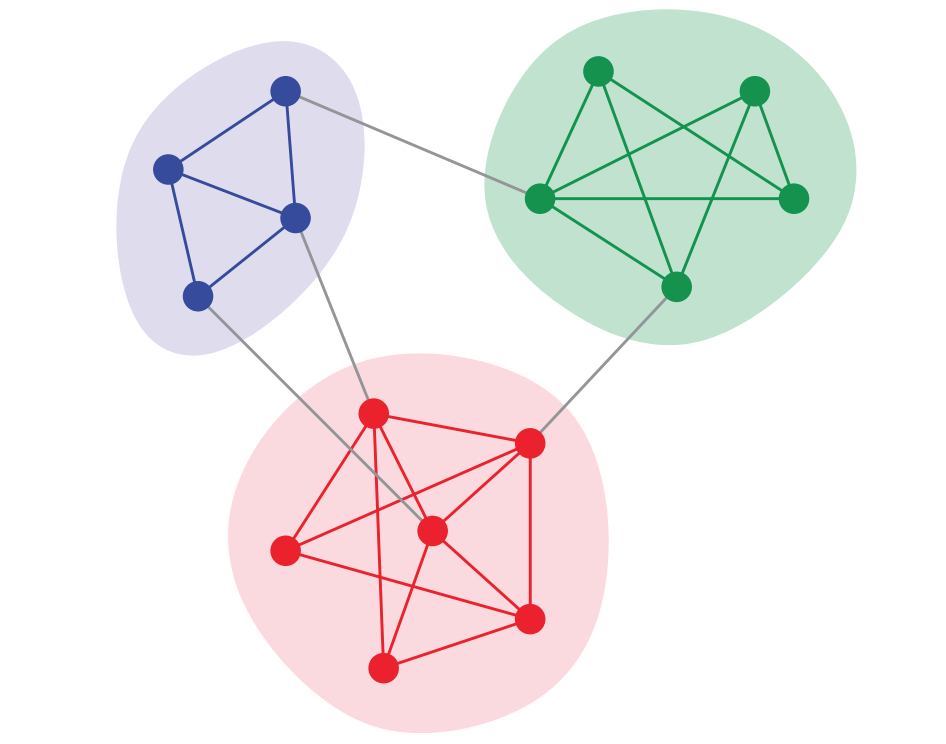
\includegraphics[width=0.5\columnwidth]{img/chapter1/community.png}
	%  \vspace{-1em}
	\caption{Example graph showing community structure. The nodes of this graph are divided into three communities, with most edges falling within communities and only a few between communities. The figure is contributed from \cite{newman2012communities}.}
	\label{fig:c1_community}
	%   \vspace{-1em}
\end{figure}
 

\begin{table}
	% \scriptsize
	\centering
	%   \vspace{-3em} 
	% \renewcommand{\tabcolsep}{2pt}
	\begin{tabular}{|p{3cm}|p{11cm}|} \hline
		\textbf{Term} &  \textbf{Definition} \\ \hline
		$G(V,E)$ & Graph $G$ with node set $V$ and edge set $E$.  \\ \hline
		$\Omega$ & $\Omega = \{ \omega_1,\omega_2,..., \omega_k\}$ is the ground truth community partition by models  where $\omega_k$ is the $k_{th}$ predicted community. \\ \hline
		$C$ & $C = \{ c_1,c_2,..., c_j\}$ is the detected community partition where $c_j$ is the $j_{th}$ community.\\ \hline
		$N, M$& $N = |V|$ denotes the node number and $M = |E|$ denotes the edge number in graph $G$\\ \hline
		$N_c$& $N_c = |c|$ is the number of nodes in community $c$\\ \hline
		$N_{c,\omega}$& $N_{c,\omega} = |c \cap \omega |$ is the common nodes in the detected community $c$ and ground truth community $\omega$ \\ \hline
		$E_{c}^{in}$& The number of edges within the community $c$. $E_{c}^{in} = \{(u,v) \in E : u \in c, v \in c \}$\\ \hline
		$E_{c}^{out}$& The number of edges on the boundary of the community $c$. $E_{c}^{out} = \{(u,v) \in E : u \in c, v \notin c$ \textit{or} $ u \notin c, v \in c \} $\\ \hline
		$D(v)$& Degree of node $v \in V$ \\ \hline
		$D_c$& The sum of node degrees in community $c$ \\ \hline
		$\mathcal{N}(v)$ & The neighbour node set of node $v$ \\ \hline
		$A$ & Graph adjacent matrix \\ \hline
	\end{tabular}
	\caption{Glossary of technical terms.}
	\label{tab:c2_glossary}
	
\end{table} 
\section{Background and Motivation}
Graph mining is one of the fundamental research areas in artificial intelligence; in the recent decade, community detection continues to be an essential topic within graph mining. Community detection approaches group nodes into communities, which can be regarded as a coarser view of a graph and reveal the latent knowledge of nodes. This detected knowledge can be used to support further tasks such as link prediction or node profile construction. For example, detecting researcher communities in a scholarly graph can imply future collaboration between them, or offer paper/research recommendations to targeted users. In biology, community structure can be used to infer possible protein-protein binding relationships, which may potentially contribute to healthcare. Therefore, exploring community detection tasks has huge practical value in both academic and industrial scenarios.

The popularity of community detection research is suggested by the thousands of papers published on the subject in top-tier journals and presented at conferences. Among these, some are survey papers which summarize state-of-the-art models from different perspectives; these have served as great references for me to organize relevant papers into different categories. \cite{fortunato2010community, fortunato2016community, coscia2011classification} are general survey papers which broadly introduce the definition of community detection and several types of models. Other papers pay more attention to detecting communities in particular types of graph. For example, \cite{malliaros2013clustering} is a classic paper which summarizes community detection in directed graphs; \cite{harenberg2014community} particularly focuses on large-scale graphs with empirical studies; and \cite{kim2015community} particularly summarizes the latest community detection models for multi-layer graphs. Still other papers focus on particular types of model frameworks. For example, \cite{abbe2017community} is the most recent work on block models in community detection. \cite{xie2013overlapping,amelio2014overlapping} are both authentic survey papers on overlapping community detection, even though they are slightly dated as of 2020.  \cite{nascimento2011spectral} is a classic research work that introduces a collection of spectral clustering models. To demonstrate how community detection supports interdisciplinary research efforts, \cite{javed2018community} and \cite{bedi2016community} show the application of community models to social media mining as well as other domains such as biology and neuroscience. Finally, \cite{chakraborty2017metrics} summarizes all types of evaluation metrics for model performance comparison. 

However, all of the aforementioned papers are either slightly out of date or relevant only to a specific topic; what is lacking is an effort to summarize and track the latest works from all possible main perspectives. This inspired me to include the most representative papers in this thesis, categorized by my own defined taxonomy. Specifically, derived from all existing works, I aim to leverage in-depth analysis in some subtle tasks and propose novel models to improve current model performance. A survey of the existing literature also inspired me to formulate and solve the various research questions mentioned in the following section.
\section{Research Problems}
In this section,I introduce three motivating tasks which this thesis aims to solve and briefly discuss my proposed approaches. The first task is \textit{Personalized Community Detection}, in which communities with different resolutions are formed given user information need. The second task is \textit{Cross-Graph Community Detection}, in which I detect pairwise user community closeness in sparse graphs by leveraging propagated information from external graphs. The third task is \textit{Community-Aware Dynamic Product Summarization}, in which community  is applied as supportive information to generate temporal product summarizations across different time periods. Details of my proposed models, along with extensive experiments and discussions, are introduced in the following chapters.

\subsection{Personalized Community Detection}
From a user-centric viewpoint, the ideal communities should provide a high-resolution partition in areas of the graph relevant to the user’s needs and a coarse partition on the remaining areas so as to best respond to the user’s needs (which can be formulated as a ``query'') in concentrated areas while leaving irrelevant areas less precisely specified. 

For instance, in Figure \ref{fig:example}, two different scholars in \textit{education} and \textit{data mining} domains, respectively, may consume the same scholarly graph differentlybecause they may need more detailed community exploration in their own domains whereas generalized community information is sufficient in irrelevant domains. For instance, a \textit{data mining} scholar may need more detailed communities in areas such as deep learning, graph mining, and Bayesian analysis, but for an \textit{education} researcher it may suffice to generalize these as computer science or even just science.

\begin{figure}
	% \setlength{\belowcaptionskip}{-10pt}
	\center
	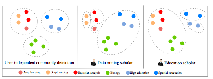
\includegraphics[width=0.8\columnwidth]{img/chapter3/example.pdf} 
	\caption{An example of personalized community detection on a scholarly graph} 
	\label{fig:example}
\end{figure}  

To solve this problem, I propose a \textbf{g}enetic \textbf{P}ersonalized \textbf{C}ommunity \textbf{D}etection (gPCD) model with an offline and an online step to efficiently cope with the time complexity issue in personalized community detection.  Details of the model structure are given in Chapter \ref{ch:personalized}.

\subsection{Cross-Graph Community Detection}
For a vulnerable graph with sparse connectivity, however, existing community detection algorithms can hardly probe enough information to optimize the community structure. Unfortunately, in real cyberspace this is a very common problem: while a handful of giant players (e.g., Google, Facebook, and Amazon) maintain high-quality graphs, thousands of apps are suffering from a “cold-start” problem in this area. If many users are isolated because of data sparseness, I can hardly determine any community information. 

To cope with this challenge, in this thesis I propose a novel research problem: Cross-Graph Community Detection. The idea is based on the fact that an increasing number of small apps are utilizing user identity information inherited from giant providers; for instance, users can easily log in to a large number of new apps using Facebook and Google ID. In such an ecosystem, the large main graph can provide critical information to enlighten community detection in many small sparse graphs. Figure \ref{fig:c4_example}depicts an example in which the Cooking and Cosmetic apps inherit important topological information from the main Amazon graph for enhanced community detection.

\begin{figure}  
	% \advance\leftskip-1cm 
	% \hspace*{0.25cm} 
	\centering
	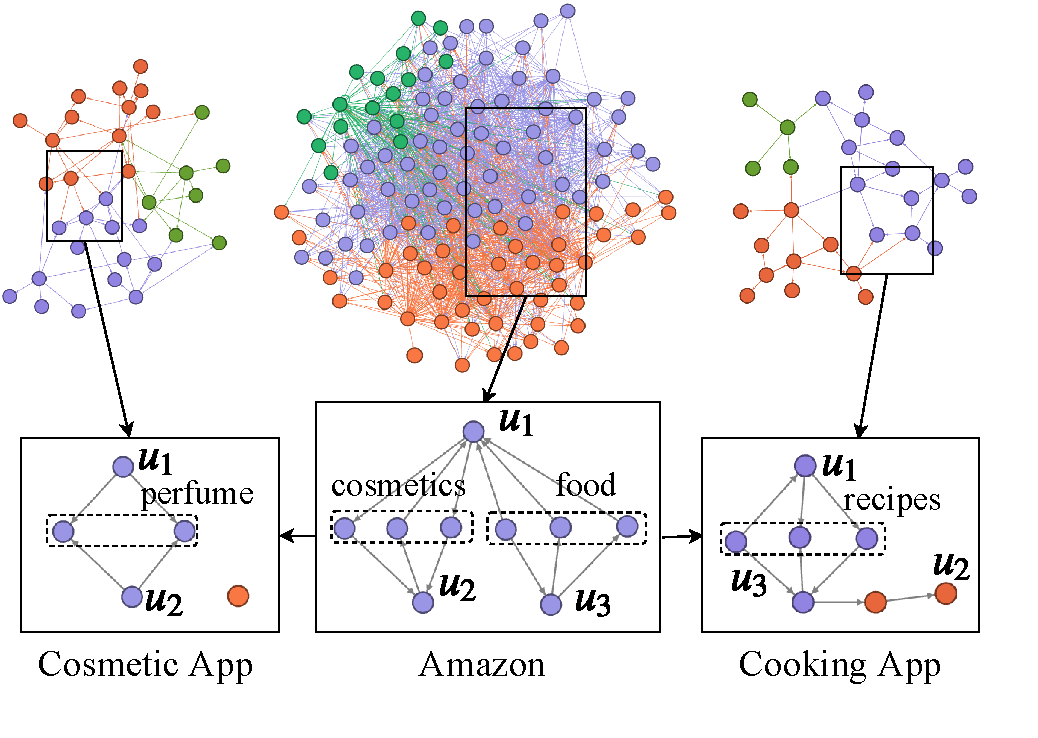
\includegraphics[width=0.8\columnwidth]{img/chapter4/example.pdf}
	%  \vspace{-1em}
	\caption{The Amazon graph is a main shopping graph while the Cosmetic App and the Cooking App are two small sparse graphs. Those graphs share mutual users in which three of them are selected to demonstrate their behaviors. Node colors indicate their related communities. }
	\label{fig:c4_example}
	%   \vspace{-1em}
\end{figure}

Inspired by the foregoing discussion, I propose an innovative \textit{Pairwise Cross-graph Community Detection} (PCCD) model for enhanced sparse graph user community detection. Specifically, given user $u_i$ and its associated triplet $\langle u_{i},u_{j},u_{k}\rangle$, I aim to predict the pairwise community relationships, e.g., compared with user $u_{k}$, does user $u_{j}$ have closer, similar or farther community closeness to user $u_i$? The details of this model structure are mentioned in Chapter \ref{ch:cross-graph}.

\subsection{Community-Aware Dynamic Product Summarization}
Product communities can implicitly reflect product characteristics. Therefore, understanding product communities and tracking their changes in a timely manner can support better decision-making for commercial purposes, such as informing online retailers in creating timely sales plans. Therefore, the \textit{Dynamic Community-Aware Product Summarization} task is of great importance. Such summarization not only indicates products’ dynamic membership changes but also utilizes these changes to depict product characteristics in readable contexts for easier interpretation.

\begin{figure}  
	% \advance\leftskip-1cm 
	\centering
	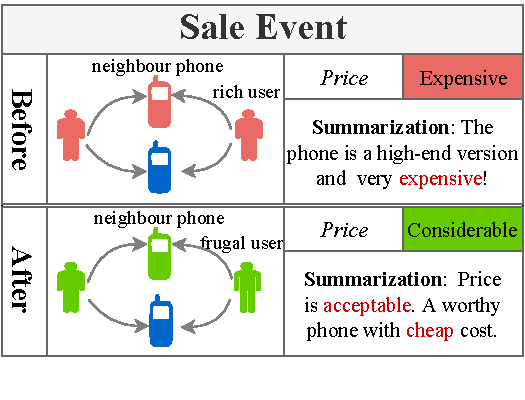
\includegraphics[width=0.8\columnwidth]{img/chapter5/example.pdf}
	% 	\vspace{-1em}
	\caption{An example to illustrate how to dynamically detect communities and select within-community neighbor products (red phone $\rightarrow$ green phone) for depicting current product (blue phone) characteristic change before \& after a sale event from user behaviors.}
	\label{fig:c5_example}
	% 	\vspace{-1.5em} 
\end{figure}

However, existing generative models relying on reviews inevitably face the sparsity issue: few products can gain enough reviews in a short time to depict the product’s temporal characteristics. User behaviors, on the other hand, are abundant and highly related to the product’s nature. Therefore, instead of review-based product summarization, I aim to generate community-aware product summarization in a dynamic manner. These approaches share the same goal but have huge differences in terms of proposed models. Review-based summarization directly runs a sequence-to-sequence model to generate product summarization by simply leveraging review context information. A community-aware product summarization, however, is generated from within-community neighbor product reviews. This means that it is a two-step approach, requiring both community detection and summarization generation.

As Figure \ref{fig:c5_example} depicts, when a sale event on a high-end phone brings frugal users' instant \textit{clicks}, behavior-based algorithms can immediately consume this information and locate updated within-community neighbor products (red phone $\rightarrow$ green phone) whose sufficient reviews help to update the product (blue phone) summarization. For review-based approaches, accumulating enough reviews to characterize this dynamic change may take a longer time. 

In the end,  I propose a  \textbf{B}ehavior based \textbf{D}ynamic \textbf{S}ummarization (BDS) model to accommodate user behavior for dynamic product summarization. The proposed model uses learned communities as a criteria to select neighbor products via a reinforcement approach, where textual review information is used to generate target product summarizations in a timely manner. Details of the model structure are given in Chapter \ref{ch:community-aware}.
\section{Contribution}
explain the contribution of this thesis such as categorizing the community detection into several forms, solve the three research questions, etc.
\section{Thesis Structure}
each chapter tells what.










%%%%%%%%%%%%%%%%
% Chapter 2
%%%%%%%%%%%%%%%%

\chapter{Related Works}  \label{ch:review}

In this chapter, I select the most outstanding studies based on a self-defined criteria (either published in a set of pre-selected venues or performed the highest impact by receiving at least fifty citations). To better introduce these papers in a well-organized manner, I categorize them into five following tracks borrowing ideas from aforementioned survey studies \cite{fortunato2010community, fortunato2016community, coscia2011classification}. In detail, papers in the Graph Type track focus on detecting communities in different types of graphs, such as heterogeneous or sparse graphs. In the Task track, the selected studies aim to solve particular tasks in community detection, such as deciding the correct number of communities. In the Methodological track, the introduced studies solve the general community detection problem via different types of model frameworks such as Modularity or spectral methods. In the Application track, selected studies discuss community detection applications and how to apply them to other disciplines. In the last Evaluation track, it lists papers to summarize the evaluation metrics widely used for model justification and comparison. 


\section{Graph Types}
Graph types are various and complex. Different type of graphs have their particular characteristics, which requires to be handled by special techniques. With the rapid development of graph mining, more and more complex graphs are constructed from real scenarios and analyzed by researchers, which offers the possibility to summarize several main types and relevant works in this section. Particularly, the following paragraphs introduce five main types of graph which are most frequently appeared in research studies and tightly connected with real-world scenarios, including heterogeneous \& multi-layer graph, sparse graph, dynamic graph, large graph and attribute graph. 

\subsection{Heterogeneous \& Multi-layer Graph} 

The research works about heterogeneous and multi-layer graph community detection are summarized together. The reason is that both types of graphs share very similar structure but still keep their own characteristics. For a heterogeneous graph, it should contains more than one type of node or edges. While for a multi-layer graph, it is composed from multiple single layer graphs. A single layer graph is with only one type of node/edge.  By connecting nodes across single layer graphs with edges, it formulates a multi-layer graph in the end. Figure \ref{fig:c2_hetero} clearly shows the definition difference between heterogeneous graph and multi-layer graph. In fact, multi-layer graph can be regarded as a particular type of heterogeneous graph. 

\begin{figure}
	% \setlength{\belowcaptionskip}{-10pt}
	\center
	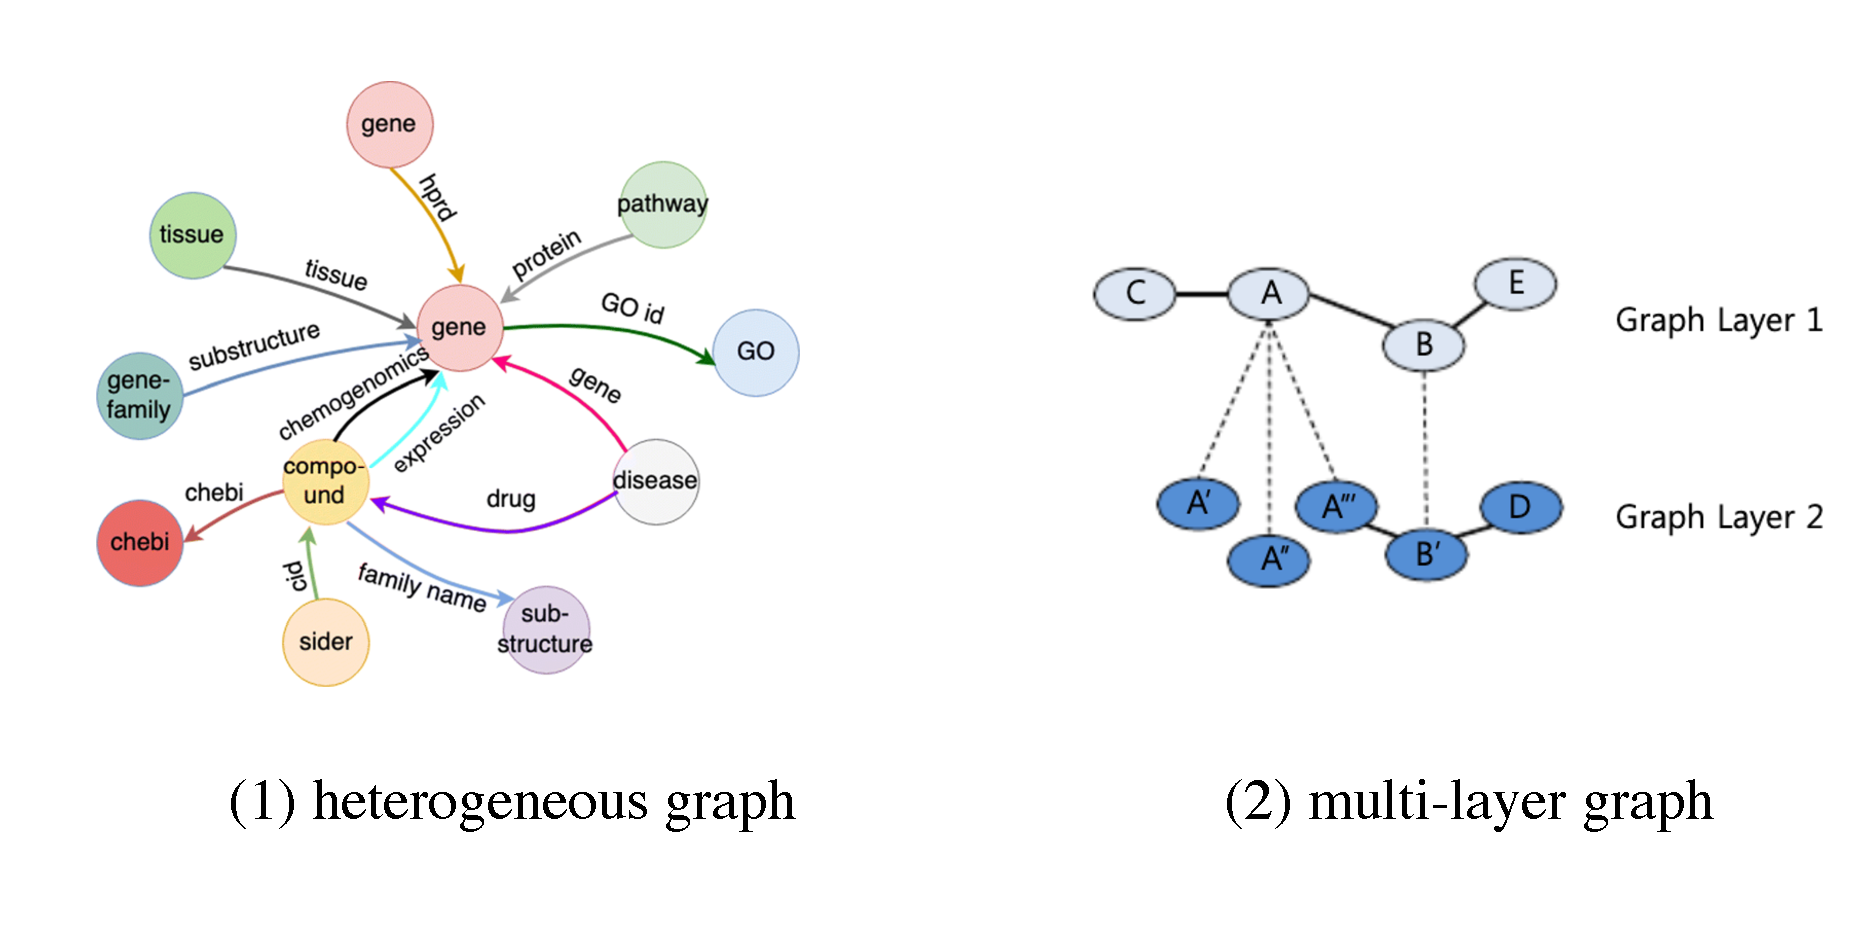
\includegraphics[width=\columnwidth]{img/chapter2/heterogenous.pdf} 
	\caption{Figure in the left is a typical heterogeneous medical graph in which nodes and edges refer to medical entities and their binding relationships from \cite{gao2019edge2vec}. Figure in the right is a multi-layer graph with two graph layers from \cite{kim2015community}.}
	\label{fig:c2_hetero}
\end{figure}  


Heterogeneous graph, also called heterogeneous information network, is a particularly complex graph which is ubiquitously appeared in current research works. By definition, a heterogeneous graph $G(V,E)$ has an extra node mapping function $\phi : V \rightarrow \mathcal{A}$ and an edge mapping function $\psi : E \rightarrow \mathcal{R} $ where each node $v \in V$ belongs to a particular node type $\phi(v) \in \mathcal{A}$ and each edge $e \in E$ belongs to a particular edge type $\psi(e) \in \mathcal{R}$. $\mathcal{A}$ is the collection of all node types and $\mathcal{R}$ is the collection of all edge types. A heterogeneous graph contains multiple node/edge types, which means at least either $|\mathcal{A}| > 1$ or $|\mathcal{R}| > 1$.

\cite{sun2013pathselclus} defines a graph structure called metapath, which is a path that connects node types with different types of edges and can be regarded as a general structure to represent path semantics. For example, a metapath in a scholarly graph can be ``Organization-(affiliated with)$\rightarrow$Author-(publish at)$\rightarrow$Venue'' where it contains three node types (``Organization'', ``Author'' and ``Venue'') and two types of edges (``affiliated with'' and ``publish at''). Particularly in this study, it integrates metapath selection with user guided clustering (a small set of nodes whose communities are known as prior information). In the end, it aims to learn the weights on selected metapaths to best satisfy the prior community knowledge via an EM approach.  

\cite{gupta2013community} introduces a joint approach to learn node affiliation distributions on popular communities in heterogeneous graph and detect node outliers which do not belong to any of the popular community distribution patterns in a holistic manner. It decomposes the heterogeneous graph into several homogeneous ones. The community detection step is derived from nonnegative matrix factorization framework and the refined outlier detection is learned via an iterative two-stage approach. In the NMF based community detection process, all prior-known community membership matrices of single node-type graphs $\{T_1,....,T_k\}$ can be used to calculate node community distribution under each node type:

\begin{equation}
	\argmin_{W,H}\sum_{i=1}^{k}||T_i - W_{i}H_{i}||^2 + \alpha \sum_{i \leq j \leq k}^{k}||H_i - H_j||^2
\end{equation}
which should subject to $W_i \geq 0$ and $H_i \geq 0$ for $ \forall i \leq k$. $W_i$ is the node vector representation matrix in the $i_{th}$ node-type graph and $H_i$ is the related community centroid matrix. The later part is the regularized term.

A node outlier score is calculated as the distance ($Dist(\cdot)$) between the current node community membership and its nearest community centroid:

\begin{equation}
S(i) =  \argmin_{j} Dist(T_{k_{(i,\cdot)}}, H_{k_{(j,\cdot)}})
\end{equation} 
Top $\rho$ nodes with largest outlier score will be regarded as outliers in current step. In an iterative learning process, the NMF method is optimized by reducing the detected outliers from the whole graph to support new node outlier detection. It stops when no outlier nodes are found out.

\cite{sun2012relation} solves a heterogeneous and incomplete graph community detection problem where only partial attribute information are given. The output of this paper includes two parts: node soft clustering distribution to indicate the probability of node affiliations to communities, and weights of edge types appeared in the graph. In model optimization, all edge types are assigned same weights in the beginning. The clustering process thereafter is applied to update the edge type weights according to the calculated average edge type consistency, which in return  guides the clustering process. The iterative process reaches to the end once all updated parameters are stable. 

Instead of node community detection, \cite{he2015stochastic} proposes an EM model for edge community detection. It aims to re-generate the whole graph by finding a partition to maximize the edge generation probabilities. Given an edge $e_{ij}$ with start node $i$ and end node $j$, its expected generation score in community $z$ is calculated as $A_{ij}^{z} = w_z\theta_{iz}\theta_{jz}$. $w_z$ is the size of community $z$ and $\theta_{iz}$ is the probability that community $z$ contains the node $i$. Then the probability of a link $e_{ij}$ belongs to community $z$ is calculated by dividing the whole generation score in all communities, as:
\begin{equation}
	R_{ij}^z = \frac{A_{ij}^{z} }{\sum_{k}{A_{ij}^{k} }}
\end{equation}
The edge $e_{ij}$ will be assigned to the community with largest generation probability. And all parameters can be learned through an EM approach.

\cite{zhou2013social} presents a social influence based framework to detect user communities in social graphs. In this paper, a social graph represents user collaborations (authors are connected by collaboration relationships) and an activity graph represents associated activity similarities (venues are connected by their topic similarities). The edges between social graph nodes and activity graph nodes represents their influence flow, such as publishing histories of authors towards venues. The three parts (social graph, activity graph and edges between them) constructs the final influence graph. First, it introduces  a new metric to  measure node similarity jointly using self-influence (social graph) and co-influence (influence graph) information. Later on, a designed SI-Cluster model takes advantage of the metric to learn node communities in the social graphs only via an Kmeans-like process. 

OCD-HSN model \cite{huang2018overlapping} detect node communities in four main steps. First, a set of seed nodes are selected according to their local minimum conductance, which enables a parallel community computation. Second, overlapping community detection is applied using local node expansion (adding and removing nodes iteratively). Third, node degrees are recalculated and normalized. Fourth, current communities are regarded as a node with coarser resolution to construct the next-level graph. Followed by all the previous steps, a hierarchical community partition can be formed in the end. 

 \cite{li2017semi} proposes a semi-supervised model to detect attribute heterogeneous graph communities by considering three types of information: node attributes, graph topological structure, and prior knowledge of must-links and cannot-links. It first calculates and assigns weights to node pairwise attribute similarity matrix and connected similarity matrix (calculated from meta-paths) to construct a node similarity matrix $S$. Then it considers the constraints (must-links and cannot-links) by assigning penalties to related node pairs. In the end, the unified model is optimized through an Expectation-Maximization (EM) framework to learn all the model parameters. 

Muilti-layer graph $G=\{G^1,G^2,...,G^k\}$ is composed by $k$ single-layer graphs $G^k= (V^k,E^k)$. For each possible pairwise single-layer graphs $G^i$ and $G^j$, there is a mapping function $\phi : G^i \rightarrow G^j$, meaning the nodes in graph $G^i$ can link to nodes in graph $G^j$, which formulates the connections between single-layer graphs. An extreme case of a multi-layer graph is that each single layer graph contains the same nodes.

\cite{kim2015community} is a short survey paper to introduce the definition of mullti-layer graph and differentiate its concept from heterogeneous graph. It offers a bunch of multi-layer graph datasets and points out several main tracks of methods, including pattern mining and matrix factorization. Typically, it introduces a popular two-layer graph community detection problem and introduces six main track methods, including cluster expansion, matrix factorization, unified distance, model-based methods, pattern mining and graph merging. 

\cite{bazzi2016community} constructs multi-layer graphs by tracking node dynamic changes across time. Therefore, each single layer graph shares the same nodes whose status and connections are changed over time. To solve the community detection in dynamic graphs, it generalizes the original Modularity method to adapt multi-layer graphs.  It also defines a persistence metric which measures the graph changes and stability across time.  

Multiplex Infomap \cite{de2015identifying} is derived from existing Infomap algorithm which originally designed for single-layer graphs. It uses codebooks to index each node and community in each layer, so that to record the paths of a random walker wandering in the multi-layer graph. The best community structure should obtains the shortest description length for the random paths. Similarly, \cite{valles2016multilayer} is also a generalized model from existing methods which is originally designed for single-layer graph community detection. Within the paper, it considers the simplest two-layer graph. It defines two type of models including an AND graph which only contains edges appeared in both layers, and a OR graph which contains edges appeared in either layers. In the end, it learns the two community partition result $C_1$ and $C_2$ in individual layers to maximize the probability to generate the AND graph from the two partitions and OR graph. 

\cite{huang2018harmonic} develops a multi-layer Modularity model by utilizing a defined graph structure called Harmonic Motif. By definition, a harmonic motif is a dense graph with largest average Z-score values in all $k$ graph layers. The Z-score shows the statistical significance of a subgraph towards the whole graph, which is calculated as:
\begin{equation}
Z = \frac{N_{real}- mean(N_{rand})}{std(N_{rand})}
\end{equation}
where $N_{real}$ is the number of time that the subgraph appears in each layer. $mean(N_{rand})$ and $std(N_{rand})$ refers to the mean and standard derivation of the number of times that the subgraph appears in a random graph with same node and number of edges.

From $k$ graph layers, the paper extracts all harmonic motifs to form a new graph layer. The existing $k$ layers are in the end coupled with the new layer to detect communities in the new graph layer by maximizing the integrated Modularity. 

\subsection{Sparse Graph}
Sparse graph is a very common phenomenon in graph mining, which is in contrary to dense graphs. However, their is no clear distinction between dense graph and sparse graph. A common notion is that dense graph is with the number of edges as $|E| = \mathcal{O}(|V|^2)$ as the maximum number of edges in a directed graph is $|V|(|V|-1)/2$. And a sparse graph usually contains the number of edges as $|E| = \mathcal{O}(|V|)$. Due to the fact that most of constructed graphs in real-world scenarios are sparse and incomplete, understanding sparse graph community detection gains a lot of practical value. 

Due to the fact that spectral clustering methods are not able to perform well in sparse graphs, \cite{krzakala2013spectral} argues that spectral methods on a refined matrix based on non-backtracking walks may achieve much better results than on the original adjacency matrix or Laplacian matrix.  The non-backtracking matrix $B$ is a $2|E| \times 2|E|$ matrix, defined as follows:
\begin{equation}
B_{(u\rightarrow v),(w\rightarrow x)} = 
\begin{cases}
1& \text{if v = w and u  $\neq$ x}\\
0& \text{otherwise}
\end{cases}
\end{equation}

\cite{chen2012clustering} designs a model for undirected, unweighted sparse graph community detection. It points out two types of clustering errors: \textit{(a)} an edge between nodes in different communities and \textit{(b)} a missing edge between nodes in the same community. These errors can be represented as an error matrix $S$ with corresponding values $\{+1,-1,0\}$. To treat the two types of errors differently, a cost matrix $M$ is utilized as well by assigning different weights on different error types. The object function thereafter is as follows to minimize the two types of errors:
\begin{equation}
	\argmin_{C,S} ||C|| + ||M \cdot S||
\end{equation}
with the restraints that $0 \leq C_{ij} \leq 1$. $C$ is the cluster matrix where $C_{ij} = 1$ if $v_i$ and $v_j$ are in the same community, and 0 otherwise. 

\cite{amini2013pseudo} claims involving perturbations in spectral clustering can improve its model performance in sparse graphs. The proposed model adds pseudo week edges between nodes to connect all disjoint components which suppose to be in the same community.  Particularly, it adds $0.25*(\lambda /|V|)$ where $\lambda$ is the average node degree in the sparse graph to each datapoint of the adjacency matrix $A$.

\cite{mirshahvalad2012significant} combines a perturbation strategy and link prediction in sparse graphs to assess all communities and select the most significant ones. As triangle is the smallest structural unit in a graph, the paper decides to complete partial of the open triangles in the original graph to achieve a denser graph. An open triangle completion means if there are two edges $e_{ij}$ and $e_{ik}$ links between a selected node triplet $<v_i,v_j,v_k>$, it will add an edge $e_{jk}$ to the original graph. By using this enhancing method, better community partition can be achieved from the denser graph. 

A rich number of researchers tend to explore sparse graph community detection from mathematical perspective. \cite{banks2016information} theoretically proves the lower and upper bound of information-theoretic threshold for community detection in the stochastic block model. The threshold is defined as $(\frac{2log(q-1)}{\lambda^2(q-1)}, \frac{2(1+\mathcal{O}(1/logq))}{\lambda})$.  $q$ is the community number, and $\lambda = \mathcal{O}(1/q)$. There will be no optimal communities for graph structure if the average node degree falls out of the threshold boundary. \cite{chin2015stochastic} is another theory paper which offers two spectral algorithms to solve sparse graph community detection model. Derived from Grothendieck’s inequality, \cite{guedon2016community} proves random graph semidefinite optimization consistency and illustrates its proofs in sparse graph community detection. 

\subsection{Dynamic Graph}

Dynamic graph, also named as temporal graph in this paper, refers to a particular type of graphs which can be dynamically changed. This graph characteristic will lead to node community evolution, which is usually happened in social media or other real-world scenarios where the user profiles and interactions are updated frequently. \cite{hartmann2016clustering} summarizes a set of relevant papers  about the metrics, tasks and datasets. It especially lists a number of papers focusing online clustering. Figure \ref{fig:c2_dynamic} illustrates a typical framework of dynamic community detection.
 
 \begin{figure}
 	% \setlength{\belowcaptionskip}{-10pt}
 	\center
 	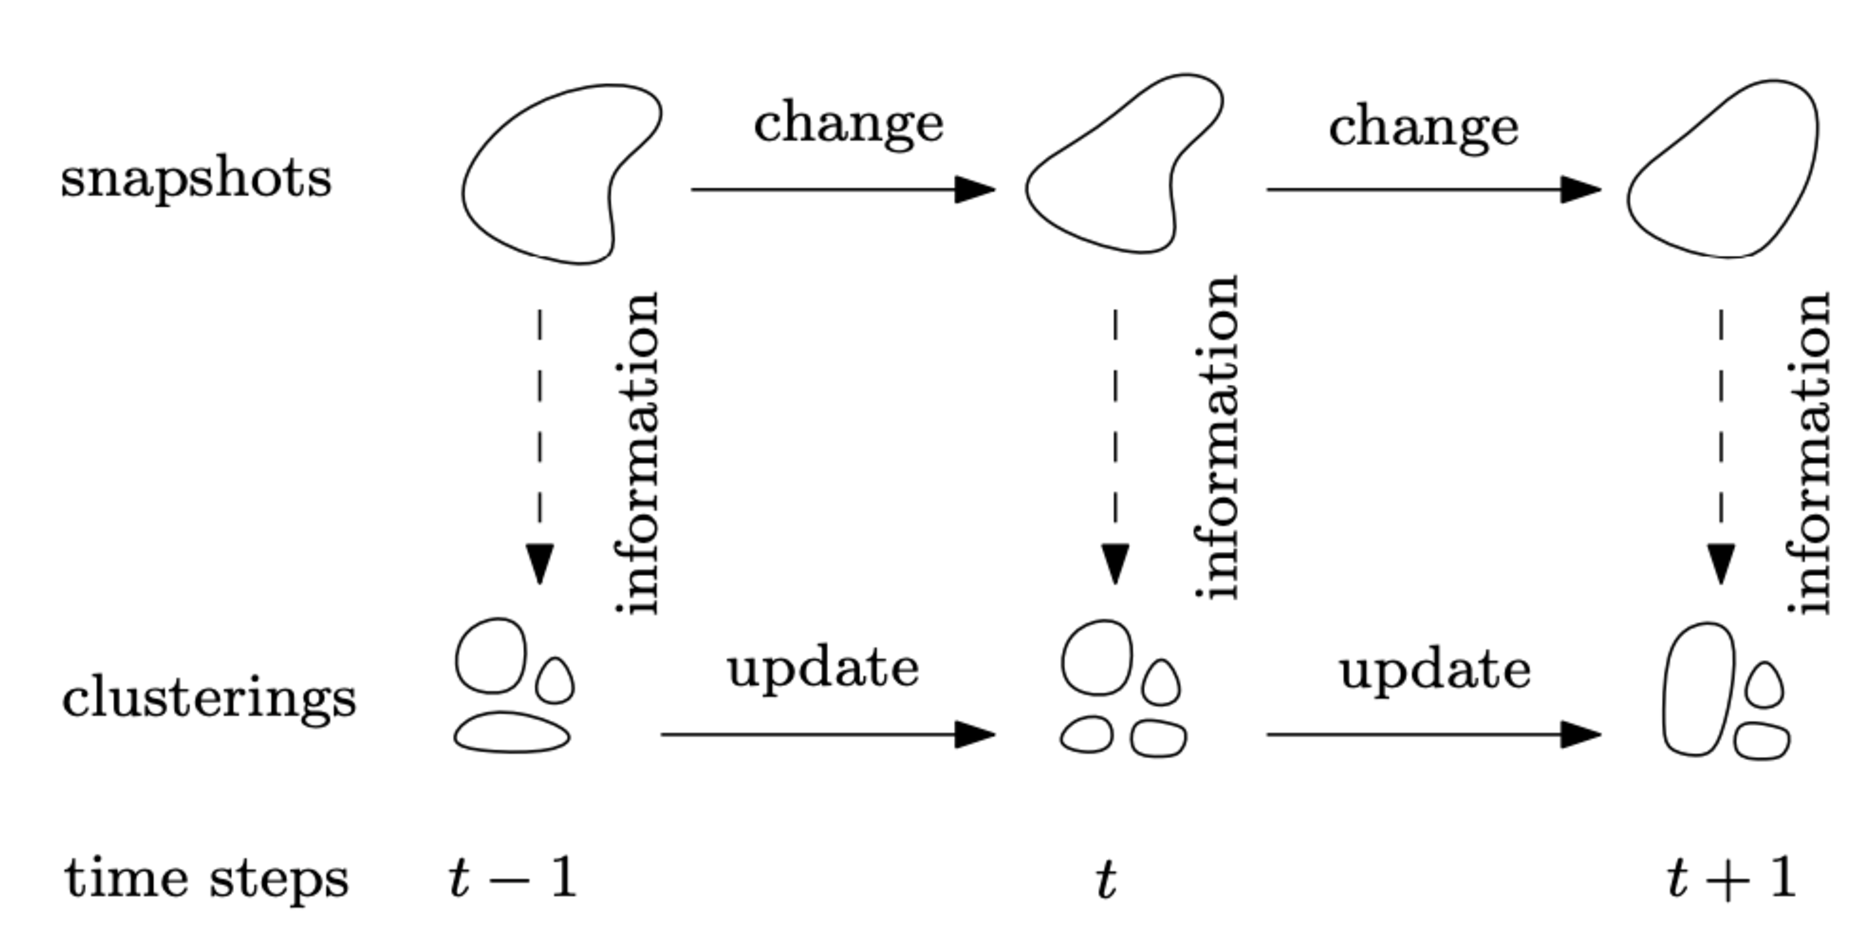
\includegraphics[width=0.9\columnwidth]{img/chapter2/dynamic.pdf} 
 	\caption{Dynamic community detection conventional steps. Figure is contributed from \cite{hartmann2016clustering}.}
 	\label{fig:c2_dynamic}
 \end{figure}  

\cite{chen2013detecting} is a classic study about dynamic community detection. It aims to learn a community matrix $C$ which best depicts the original graph adjacency matrix in a weighted form across all timestamps:
\begin{equation}
	\min_{Y}\sum_t \sum_{i,j}|A_{ij}-\frac{N_i N_j}{2|E|}||Y_{ij}-A_{ij}|
\end{equation}
where $Y=CC^T$.

DYNMOGA model \cite{folino2013evolutionary} is a genetic based approach to detect smooth communities with multi-object optimization. It considers the accuracy of the generated communities in the temporal graph at each timestamp. Meanwhile it also tries to minimize the transformation cost between two community partition results in consecutive timestamps. 

\cite{xu2014dynamic} combines two statistical models: a static model for individual graph snapshot in each timestamp and a temporal model to track the evolution of states. It proposes a prior \& posterior stochastic block model, in which the previously learned parameters in the last snapshot are used to optimize the current community memberships via  extended Kalman filter (EKF). Using similar approaches, SBTM model \cite{xu2015stochastic} leverages hidden Markov assumption in original SBM in which the presence/absence of an edge between two nodes will directly influence whether it will appear again in the next timestamp. 

NEIWalk model \cite{wang2013neiwalk} is a random walk method applied on dynamic content-based graphs by tracking the evolution of both graph structure and node/edge content.  In detail, the model transforms the original graph into a Node-Edge Interaction (NEI) graph which contains two types of nodes and three types of edges. In NEI graph, the two node types are the node and edge in the original content-based graph. And the three edge types are the calculated structural similarity, node content similarity and edge content similarity. The dynamics in the original content-based graph is reflected to the structure evolution in the NEI graph. To detect communities in each timestamp, a random walk based model is proposed to involve a transition probability matrix between each node/edge type and thereafter detect communities in the NMI graph. 

\cite{appel2018temporally} also detects dynamic communities in content-based graphs by incorporating graph structure, content and temporal analysis in a shared matrix factorization model. In each timestamp, it considers to learn three following matrices in a holistic way: a matrix $U_t$ at timestamp $t$ based on both structural and content information, a global  matrix $S$ based on structural information and another global matrix $W$ based on content information across all timestamps. The objective function uses these three matrices to best estimate the original adjacency matrix $A$ and given content matrix $C$:
\begin{equation}
\argmin \sum_{t}||A_t-U_tS^T||^2 + \beta\sum_{t}||C_t-U_tW^T||^2 + \lambda(||S||^2+||W||^2+\sum_t||U_t||^2)
\end{equation}
The first  term aims to estimate $A$, the second term aims to estimate $C_t$ at each timestamp $t$, and the third term is the regularization term  to avoid bias and overfitting.

\cite{wang2013dynamic} focuses on dynamic community detection in graph streams by defining a Local Weighted-Edge-based Pattern (LWEP), which is a subset of node densely connected in local regions. The whole approach is divided into online and offline steps. In the online step, for each node in timestamp $t$, a top-k neighbor node list (with largest edge weights) and a top-k candidate node list (with highest burst activities) are extracted to preserve graph main structure. In the offline step, the LWEPs are created in each timestamp from online results. A straightforward two-step approach first cleans the generated LWEPs and then uses a breadth first search (BFS) method to figure out dynamic community structures.  

\cite{kim2013nonparametric} proposes a nonparametric multi-group membership model for dynamic graphs. Within its model, a community can be tracked as either active or inactive, which is assumed to follows Poisson distribution. In timestamp $t$, the dynamic joining or leaving of a node towards a community is estimated by a Markov chain process considering its previous status in the community. The estimated parameters follow Beta distribution. The community structure can be used to estimate the probability of edge affinities in the original graph. Finally a MCMC method is used to optimize all the to-be-learned parameters under all assumed distributions.

\cite{ghasemian2016detectability} is a theoretical paper which argues a threshold generated from community strength and dynamic change rate. It claims that there would be no effective methods if the dynamic graph has a score below the threshold. Further more, it mathematically proves belief propagation model and spectral clustering are able to detect reliable communities if the graph structure is above the threshold.  

\cite{yang2018poisson} is another statistical work which assumes evolved node-community memberships following Gamma distribution. The communities also follows a Gamma distribution. The edges between nodes follow Bernoulli distribution and their weights follow Poisson distribution. The whole process optimizes all aforementioned distributions through a MCMC process. Similarly,  \cite{peixoto2017modelling} uses Bayesian Markov Chain to generate sequential edges appeared in the graph without specified time windows. 

\cite{delvenne2010stability} introduces a new metric, stability, to assess community partitions. The stability of a community partition is defined as:
\begin{equation}
	r(t,C) = \min_{0 \leq s \leq t} trace[C^T(\Pi M^t -\pi^T \pi)C]
\end{equation}
where $M$ is the node transition matrix, $\pi$ is the normalized degree vector over all nodes and$\Pi = diag(\pi)$ is the corresponding diagonal matrix. $C$ is the community  matrix. The partition with maximized stability may not be the best one in current timestamp. But its community structure should be with good coherence in a relative long time period.

In \cite{gauvin2014detecting}, the time-evolving graphs can be represented as a set of sequential adjacency matrices, which can be integrated as a three-way tensor $\mathcal{T}$. The conventional matrix factorization can be thereafter applied to the tensor by finding three low dimensional matrices $A,B,C$ to best estimate $\mathcal{T}$. $A$ and $B$ provides the graph community structure and $C$ represents the temporal activity of communities. It is a PARAFAC decomposition problem to solve.
\begin{equation} 
\min_{A,B,C} ||\mathcal{T} - A,B,C||^2_F
\end{equation}

\cite{tang2011identifying} focuses on dynamic multi-mode graphs, which is a particular type of heterogeneous graph where the node types and edge connections are constructed from different modes such as text and videos. It uses a matrix factorization approach to learn node community matrix in each timestamp by estimating the interaction between each pairwise modes. And a side effect from snapshot graph in the last timestamp are also considered in the learning process.

\subsection{Large Graph}

Large scale graphs are ubiquitous in various domains. Especially in recent years, with the increasing computation capability, more and more researches focus on how to deal with large graph community detection. A well-known survey paper \cite{harenberg2014community} introduces a number of methods focusing on both overlapping and disjoint community detection as well as many frequently used metrics and datasets for evaluation.

TopGC model\cite{macropol2010scalable} proposes a linear-time searching algorithm to detect the best community instead of the entire graph communities. It uses the idea derived from Locality Sensitive Hashing (LSH) to index nodes and find the communities with largest cluster scores (related to the community size and number of within-community edges). \cite{spielman2013local} is another local searching model which leverages random walks to detect the best community for each given node, and runs in approximately linear time. 

\cite{satuluri2011local} introduces a novel model to deal with large graphs by sparsifying graphs and removing unimportant edges to maintain the main graph structure. Once the graph size is reduced, the running time of most methods will be shortened as their complexity are always related to the graph size. To prune the graph in an efficient manner, a local sparsification algorithm is introduced to maintain the top ranked edges (edge score is calculated by the Jaccard Similarity of current node and the other endpoint node) per node. A further threshold is set up to ensure the pruned graph is still connected. 

\cite{wang2011detecting} formulates a novel problem, community kernel detection, which contains two tasks: find the most influential users and detect their community structure.
It proposes two separate algorithms, GREEDY and WEBA, both to solve the two tasks in a unified framework. In the GREEDY method, it firstly initializes a set of seed nodes as kernel communities. Then these communities expands by merging nodes with closest connections. In the WEBA method, the model learns a weight vector for each node to represent its belonging score to each community. The weight vectors are learned by maximizing the inner product of the vector of all pairwise connected nodes.

GEM model \cite{whang2012scalable} is proposed to cluster large-scale social networks. It consists of three steps: firstly it extracts the main skeleton from the original graph, and then detects the  skeleton graph communities via a k-means method, in the last step the calculated result is propagated back to refine the communities of entire graph. In detail, for graph extraction,  all nodes whose degree are above a threshold are selected and their edges are kept. Then a weighted k-means with refined seeding strategy is applied to cluster the filtered skeleton graph.  In the end, the remained nodes in the original graph are assigned to the generated communities through a breadth first search (BFS) approach.

\cite{li2013efficient} gives a novel definition of a community in which all nodes are closer to the current community centers than to the rest communities. After that, two new algorithms (Cores-Aware and Cores-Unaware algorithm) are proposed to detect communities in linear time. The Cores-Aware algorithm is leveraged under the condition that community cores are known. Then a breadth first search (BFS) approach is applied to calculate other node distances towards all cores and assign their communities. In the Cores-Unaware algorithm, their is no prior-known community cores. 

ESCG model \cite{liu2013large} repeatedly generates supernodes with coarser resolution to replace the original nodes in bipartite graph, which reduces the original graph size and accelerate the running speed. In detail, the model first randomly picks up a number of seed nodes as individual supernodes. Then a BFS approach is taken to allocate the rest nodes to the seed nodes based on their shortest paths. In the end, a standard spectral clustering method is leveraged on the reduced graph to detect communities. 

\cite{de2014mixing} proposes a mixed global and local method to bump up the efficiency via a defined k-path edge centrality as a substitution of the original edge betweeness centrality. Each edge importance score is calculated via random walks, which maps nodes to a latent space and calculates all pairwise distances for final community detection. The k-path edge centrality is defined as:
\begin{equation}
	L^k(e_{ij}) = \sum_{v \ V} Pr(e,v)
\end{equation}
It calculates the sum of probabilities that a k-step random walk passes edge $e_{ij}$ which is originally started as node $v$. And the distance of pairwise nodes can be thereafter calculated as:
\begin{equation}
	d_{ij} = 1 - \sqrt{\sum_{v \in V}\frac{(L^k(e_{vi})-L^k(e_{vj}) )^2}{d(v)}}
\end{equation}
The Louvain method is finally applied on the all pairwise node distances to calculate their communities.

\cite{kollios2013clustering} deals with large probabilistic graphs in which each edge is associated with a probability to appear or not appear. It proposes a simple model to generate a cluster graph $C$ which has the least edit distance with the original graph $G$. And the disjoint subgraphs in the cluster graph $C$ naturally form the communities.

SCD model \cite{prat2014high} is a scalable approach to detect communities by maximizing the Weighted  Community Clustering (WCC) metric. It also allows to run in parallel, which achieves a two-order magnitude acceleration in terms of running speed. WCC is defined based on the intuition that nodes should have a higher chance to form triangles with in-community nodes compared with the out-community nodes. Therefore, for a given node $v$, its WCC score in a community $c$ is calculated as:

\begin{equation}
WCC(v,c) = 
\begin{cases}
\frac{t(v,c)}{t(v,V)} \cdot \frac{vt(v,V)}{|c - v| + vt(x, V-c)} & \text{if t(v,V) $\neq$ 0}\\
0& \text{if t(v,V) = 0}
\end{cases}
\end{equation}
$t(v,c)$ and $t(v,V)$ refer to the number of triangles containing node $v$ in the community $c$ or the whole graph nodes. $vt(v,V)$ refers to the number of nodes that forms close triangles with current node $v$. The sum of all nodes' WCC scores across all communities is the final score to evaluate the fitness of current partition. The paper uses an iterative approach to learn the community partition with largest WCC score. \cite{tsourakakis2017scalable} also takes advantage of closed triangles in a spectral clustering approach.

\cite{li2015uncovering} aims to find overlapping communities in large-scale graphs. It defines a local spectra which uses a set of seed nodes (with known communities) as the dimensions to represent all other nodes through random walks. The local spectra representation hugely reduces the workload to decompose the adjacency matrix. And a refined k-means method helps to group nodes into overlapped communities. 

DFuzzy model \cite{bhatia2018dfuzzy} leverages deep learning techniques in four steps. First, it uses a PageRank method to initialize the potential community centers. Second,  PageRank based clustering encodes node hidden representations by maximizing graph Modularities. Communities are detected in the decoding process by minimizing the reconstruction error in the unified encode-decoder framework.

Some other studies are relevant to large-scale graphs from different perspectives. \cite{hallac2015network} is a theory paper which introduces network lasso to enhance the optimization process. \cite{jeub2015think} is an empirical paper aims to identify under what scenarios that small communities are better/equal/worse than large communities. \cite{peixoto2015model} offers a model selection strategy by considering graph minimum description length. 

\subsection{Attribute Graph}

\begin{figure}
	% \setlength{\belowcaptionskip}{-10pt}
	\center
	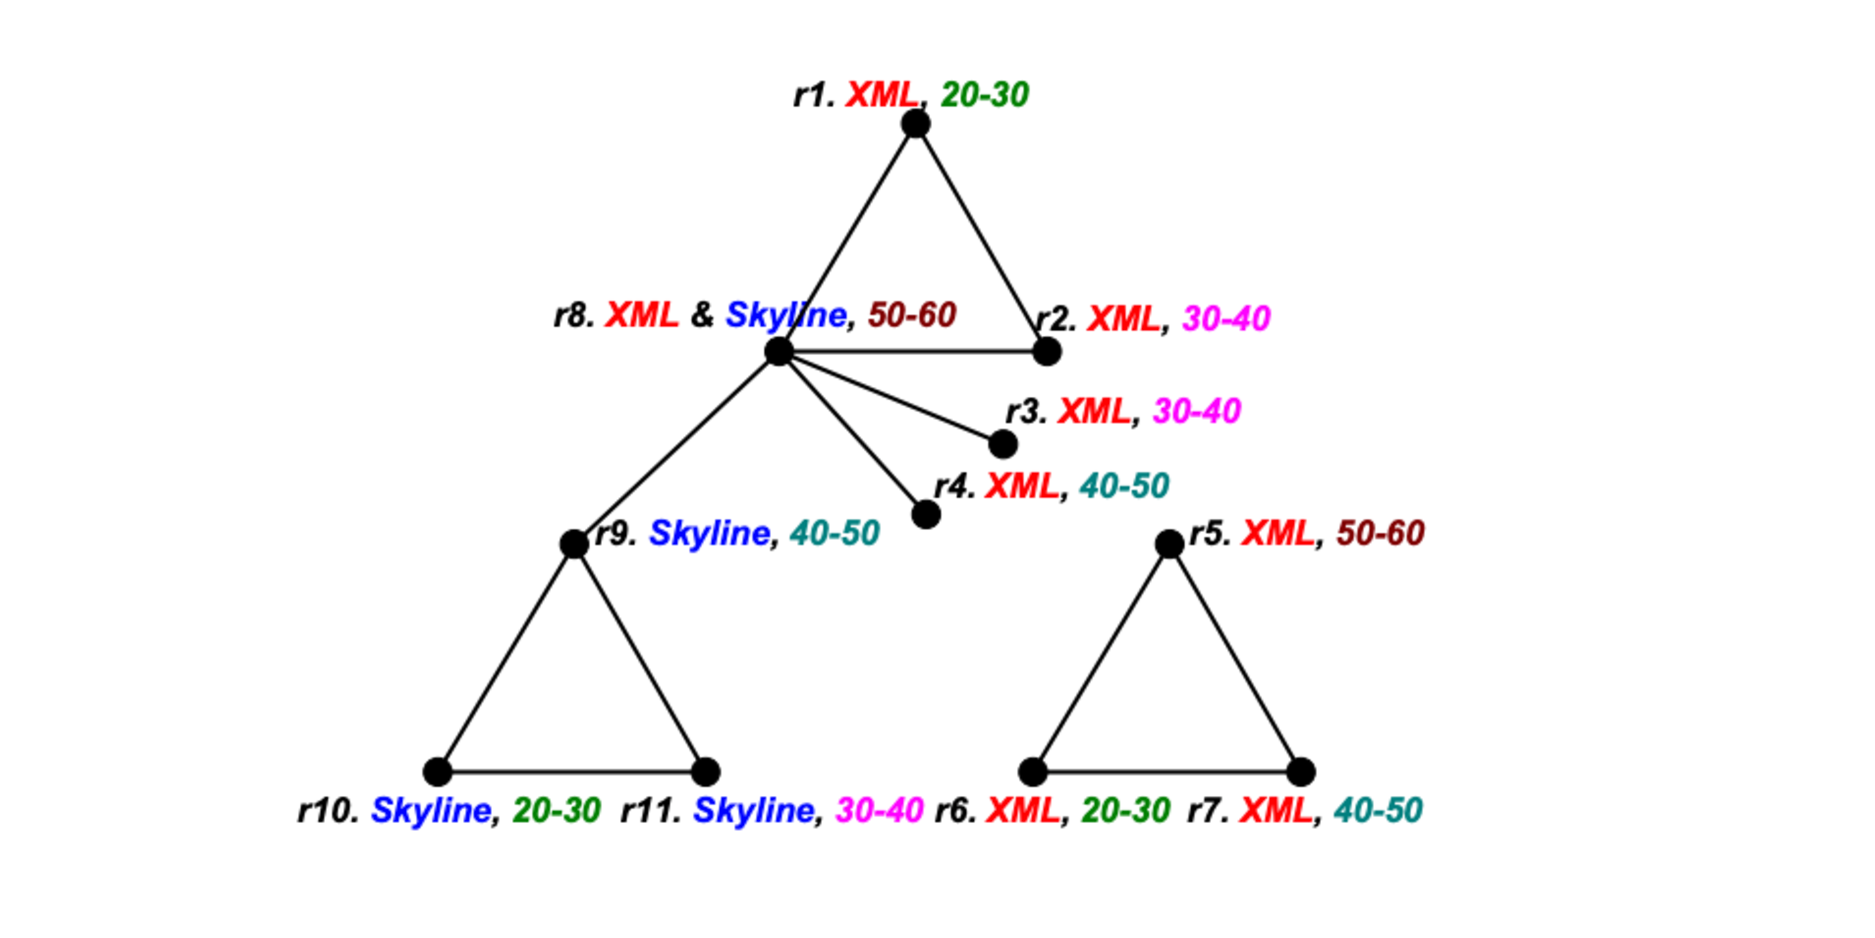
\includegraphics[width=\columnwidth]{img/chapter2/attribute.pdf} 
	\caption{A co-author graph with two attributes ``Topic'' and ``Age''. Figure is contributed from \cite{yang2013community}.}
	\label{fig:c2_attribute}
\end{figure}  


Intuitively, attribute graph is a type of graph in which nodes contains extra information. Figure \ref{fig:c2_attribute} shows a typical attribute co-author graph with ``Topic'' and ``Age'' attributes. An attribute graph $G(V,E)$ is associated with an attribute collection $\Lambda=\{ \lambda_1,...,\lambda_m\}$ containing $m$ different attributes.  Each node $v$ is associated with an attribute vector $[\lambda_1(v),...,\lambda_m(v)]$ where $\lambda_1(v)$ is the attribute value of node $v$ on attribute $\lambda_m$. A more complex attribute graph can involve attributes in edges as well with similar representations to node attributes.  Bayesian approaches and nonnegative matrix factorization approaches are the two main tracks of methods, and their related works are summarized in Table \ref{tab:c2_attribute}.

\begin{table}
	% \scriptsize
	\centering
	%   \vspace{-3em} 
	% \renewcommand{\tabcolsep}{2pt}
	\begin{tabular}{|p{5cm}|p{9cm}|} \hline
		\textbf{References} &  \textbf{Main Idea} \\ \hline
		\cite{xu2012model,han2015probabilistic,bojchevski2018bayesian,he2017joint} & Bayesian generative \& probabilistic model\\ \hline
		\cite{qi2012community,wang2016semantic,qin2018adaptive,}& Nonnegative matrix factorization\\ \hline
		\cite{zhang2019attributed,jin2019graph}& Graph convolutional network \\ \hline 
		\cite{zhou2010clustering,pool2014description,yang2013community,huang2015dense}& Others\\ \hline 
	\end{tabular}
	\caption{The main ideas of mainly introduced attribute graph community detection approaches.}
	\label{tab:c2_attribute}
	
\end{table} 


Inc-Cluster model \cite{zhou2010clustering}  uses random walk distance matrix instead of adjacency matrix to calculate node communities. The random walk distance matrix considers the random walk probability between each pair of nodes and their involved attributes. Thereafter, a Kmeans-like method is taken to initialize community centroids and run with the four following steps iteratively until convergence: first,  it assigns nodes to the community with the nearest centroid random walk distance; second, it updates each community centroid from the newly formed communities; third, it adjusts attribute weights with an efficient incremental method; fourth, it re-computes the random walk distance matrix and starts the next iteration. 

SCMAG model \cite{huang2015dense} aims to retrieve the dense communities from attribute graphs. It firstly leverages an entropy-based method to find dense subspaces. A random walk based method calculates the structural closeness and attribute similarity between communities together as a unified metric. A combining strategy is finally proposed based on the metric to merge subspaces together as communities. 

\cite{xu2012model} seamlessly captures both structural and attribute aspect information and develops a Bayesian probabilistic model to detect node communities. It leverages three matrices including adjacency matrix $X \sim Bernoulli(\cdot)$, attribute matrix $Y \sim Multinomial(\cdot)$ and node community label vector $Z \sim Multinomial(\cdot)$. The overall generative process firstly samples the community label for each node. Then given the community label and node itself, the model samples node attributes. In the end, given community labels for each pair of nodes, the model samples whether there is an edge between them. The overall idea is to reproduce the original graph by optimizing these three generation probabilities.

CRM model  \cite{han2015probabilistic} is also a probabilistic model to incorporate all user information from social networks. The overall approach aims to generate three types of user information including community (each edge belongs to a community), role (each node can have multiple roles) and action (edge node can take multiple actions such as transferring a message). The three generative process are interacted with each other and optimized through an EM approach. 

PAICAN  \cite{bojchevski2018bayesian} is a jointly model which learns partial node anomalies and communities via a statistical inference perspective. A node is a partial node anomaly when it is an outlier in at least one attribute. In the graph generative process, an edge is generated from different distribution assumption under three case of endpoint node information: both nodes are good,  one endpoint node is good, and both nodes are anomaly. \cite{he2017joint}  is another model involving node semantics. Similarly, the overall process is a joint community $\rightarrow$ edge generation and topic $\rightarrow$ attribute generation model.
 
\cite{pool2014description} aims to detect top $k$ communities which can both group cohesively connected nodes together and concisely describe their attributes. It defines two types of errors to assess community partition fitness. The first type error is missing edges between nodes in the same community. The second type error is the edges existing between communities. The model calculate the scores of community given these two criteria. The idea of this paper is to generate concise queries from node attributes and selects top $k$ best fit communities for these queries. 

CESNA model \cite{yang2013community} detects overlapping communities by considering both edge structure and node attributes. It is a scalable algorithm with linear running time. The intuition behind CESNA model is that node community memberships should be able to indicate node attributes. The probability that a node $u$ contains attribute $k$ is described as:
\begin{equation}
	P_{uk} = \frac{1}{1+exp(\sum_c W_{kc}\cdot F_{uc})}
\end{equation}
where $F_{uc}$ is the affiliation score that node $u$ belongs to community $c$. Weight $W_{kc}$ is the weight factor for attribute $k$ towards community $c$.

\cite{qi2012community} shows how edge content can be used to improve the effectiveness of community detection. The overall model is derived from matrix factorization. It considers to minimize both structural object and edge content object in a unified function $\mathcal{O}(E)$:

\begin{equation}
\mathcal{O}(E) = ||E^TE\Delta - \Gamma||^2_F - \lambda tr(E^TLE)
\end{equation}

The first part is the structural object to minimize, where $\Gamma$ is a $|E|\cdot|V|$  matrix to encode edge and node underlying structure. $\Gamma_{ij} = 1$ if $v_j$ is the start-or end-point of $e_i$. Otherwise $\Gamma_{ij} = 0$. $E$ is a low dimensional matrix representation for all edges. $\Delta$ is a  $|E|\cdot|V|$  matrix whose entry $\Delta_{ij} = \frac{1}{d(vj)}$ if $v_j$ is the start-or end-point of $e_i$. The second part is the edge content object. $tr(\cdot)$ denotes the trace of relevant matrix. $\lambda$ is a weighting factor. $L$ is the normalized Laplacian matrix storing all pairwise edge content similarities. In the end, edge vectors are learned  and used for community detection.

\cite{wang2016semantic} aims to learn a community membership matrix $U$ and community attribute matrix $C$ through a nonnegative matrix factorization framework. The objective function in this model is defined as:
\begin{equation}
	\argmin_{C \geq 0, U \geq 0}||U-SC||^2_F + \alpha\sum_{j=1}^{k}||C(:,j)||^2_F + \beta ||A-UU^T||^2_F
\end{equation}
where $U_{ij}$ is the propensity of node $i$ belongs to community $j$. $C_{qr}$ is the propensity of that attribute $q$ belongs to community $r$. $S$ is the given node attribute matrix. The first term aims to estimate node community membership matrix from node attributes. The second term is an add-on bias. The third term is to use community membership matrix to estimate the original adjacency matrix $A$.

\cite{qin2018adaptive} incorporates node content into a nonnegative matrix factorization approachc and use a weight matrix $C$ to control the impact of the attribute information for community detection. The objective function it aims to optimize is as:
\begin{equation}
\argmin_{X \geq 0,Y \geq 0} \alpha ||A-XX^T||^2_F + ||X-CY||^2_F
\end{equation}
where $A$ is the adjacency matrix, $X$ is the community membership matrix, $Y$ is the community attribute matrix to describe how much likely the community can be described by each attribute. $C$ is the node attribute matrix. Both $X$ and $Y$ are the matrices to be learned. 

\cite{zhang2019attributed,jin2019graph} are both deep-learning based method to involve node attribute into graph convolution process and trained in an end-to-end manner.

\subsection{Summary}
In this section, I introduce five different types of graphs and a bunch of related research works. Some of the graph types are commonly seen in real-world scenarios such as sparse and large graphs. Effective and efficient models on such graphs can produce huge practical value to reduce online latency and required machine memories. Researches in attribute graph is becoming more popular because it can involve extra information to support graph partition. The extra information is always with meaningful semantics, clear format and easy to be obtained.  Besides the type of graphs introduced in this section, there are also other types of works, such as signed graph and hypergraph, which are all interesting topics and deserves more future exploration.  
\section{Tasks}
In this section, research works about five  popular community detection tasks are summarized. The five selected tasks are independent with each other and tackle community detection problems from various perspectives. 

\subsection{Overlapping Community Detection}
\begin{figure}
	% \setlength{\belowcaptionskip}{-10pt}
	\center
	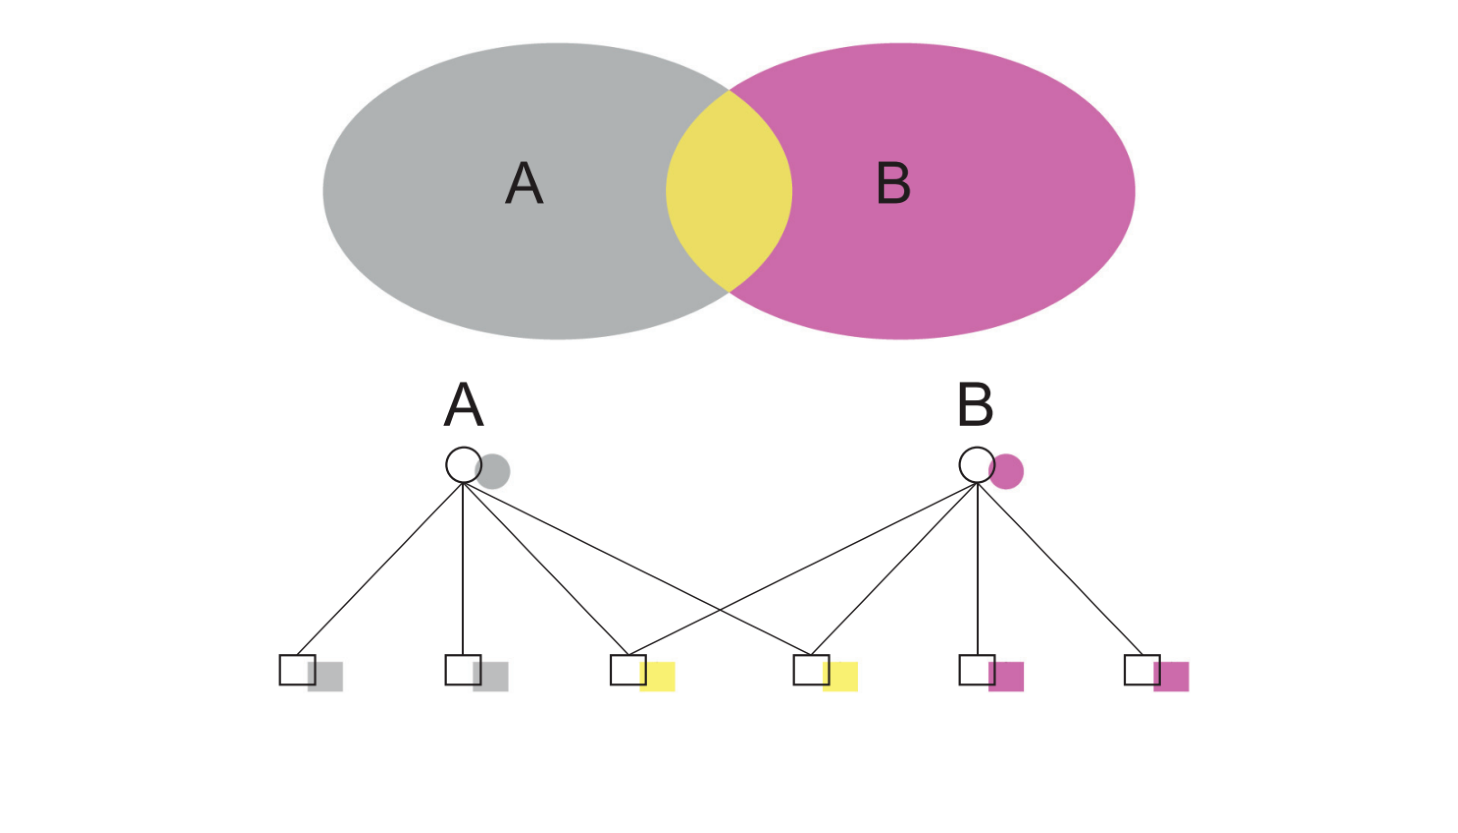
\includegraphics[width=\columnwidth]{img/chapter2/overlapping.pdf} 
	\caption{Overlapping Community Structure where nodes can belong to multiple communities. The figure is contributed from \cite{yang2013overlapping}.}
	\label{fig:c2_overlapping}
\end{figure}  


Overlapping community detection is one of the most fundamental topics and many relevant studies are published. By definition, a node $v$ can belong to multiple communities simultaneously so as to cause the overlaps between communities. Figure \ref{fig:c2_overlapping} visualizes the community structure under overlapping circumstance. The nodes marked in color yellow are affiliated with both community $A$ and $B$. Table \ref{tab:c2_overlapping} categorizes and summarizes the focus of each mentioned study for overlapping community detection.

\begin{table}
	% \scriptsize
	\centering
	%   \vspace{-3em} 
	% \renewcommand{\tabcolsep}{2pt}
	\begin{tabular}{|p{5cm}|p{9cm}|} \hline
		\textbf{References} &  \textbf{Main Idea} \\ \hline
		\cite{coscia2012demon,whang2013overlapping,whang2016overlapping,huang2018overlapping,wang2017overlapping} & Local search and seed expansion\\ \hline
		\cite{yang2013overlapping,zhang2015incorporating,zhang2016modeling,eustace2015overlapping,jin2015combined}& Nonnegative matrix factorization\\ \hline
		\cite{gopalan2013efficient,jin2016detect,}& Bayesian, generative model\\ \hline
		\cite{yang2012community}& Affiliation network\\ \hline
	\end{tabular}
	\caption{The main ideas of mainly introduced overlapping community detection approaches.}
	\label{tab:c2_overlapping}
	
\end{table} 

\cite{amelio2014overlapping} is a survey paper published in 2014. Although the methods introduced within it are sort of dated, it still offers covers several main track methodologies (node seed and local expansion, clique expansion, and label propagation) and particular scenarios (link clustering and dynamic graphs). It draws a conclusion that there is no universal method to deal with all types of graphs with different characteristics in sparsity, degree distribution, and overlap percentage among communities. In the end, it also points out two essential questions to be solved for later researchers, which is ``when to apply overlapping methods and how significant the overlapping is''.  \cite{xie2013overlapping} is another authentic survey paper which reviews a set of methods, benchmarks and evaluation metrics. Besides that, it also reviews papers using stochastic block model or density based models. To study the performance differences among models,  it introduces several benchmark graphs in which node ground truth community is known, i.e. LFR benchmark graph\footnote{https://sites.google.com/site/andrealancichinetti/files}. A set of evaluation metrics including Normalized Mutual Information (NMI) and Omega index are introduced as well. Meanwhile, empirical studies are applied and evaluated on all aforementioned methods using different benchmark graphs. In the end, the paper discovers the sensitivities of different models in sparse graphs appeared in real-world social networks.

DEMON model \cite{coscia2012demon} unveils its overlapping communities with a local-first approach by grouping ego neighbor nodes into the same clusters and finally merges the local communities into a global collection. In the local-first grouping process, DEMON applies a EgoMinusEgo function to first extract ego-based subgraphs for each node $v$ where the node set is node $v$ and all its neighbor nodes $\mathcal{N}(v)$  and the edge set is all graph edges between the selected nodes ($v$ and $\mathcal{N}(v)$). After that, each ego-based subgraph will remove the node $v$ and all its associated edges to achieve an EgoMinusEgo subgraph. An label propagation community detection method is subsequently applied on each EgoMinusEgo subgraph and select a set of largest clusters to best cover the entire graph. In the end, a merging process is applied on the previously generated clusters according to their node similarities and construct the final community partition result. LOSP model \cite{he2015detecting} is another method to explore local neighborhood structures of each node. It defines a Local Spectral Subspace using the first $d$ eigenvectors from the normalized adjacency matrix. In each potential community $c$, a set of seed nodes are given, and an iterative process is applied with the help of seed nodes and the Local Spectral Subspace to rank the top $N_c$ nodes with highest random walk probabilities to appear in the current community. Those nodes are finally regarded as other latent members in each community $c$. 

LOSP model offers a great insight to use seed node expansion to detect overlapped communities. Inspired by LOSP model, \cite{whang2013overlapping,whang2016overlapping} propose a four-phase model including filtering, seeding, seed set expansion, and propagation. The natural of the model first filters out the regions of the graph which don't involve overlapping structure. A seeding strategy inspired by Kmeans selects a set of seed nodes with small Conductance relationship. A seed set expansion approach is further applied by taking advantage of personalized PageRank model to construct raw communities near each seed node. In the last propagation step, the raw communities are expanded again to the regions previously removed in the filtering phase. Similarly, \cite{yang2017finding} also designs a new seeding strategy and expands a set of nodes from seed nodes via a personalized PageRank model. Thereafter it develops a model on the expanded nodes to detect overlapped communities. The seed nodes are the nodes in the maximum spanning tree of the original graph. Personalized PageRank model helps to expand the seed nodes and merge them into raw community structure by maximizing modularity score of the graph. The last optimization step is to merge communities when the shared node ratio of two communities is above an overlapping threshold.

OCD-HSN model \cite{huang2018overlapping} contains a seed selection step as well as community initialization and expansion step to group nodes into clusters in an efficient manner. It claims to be the first research work for overlapping community detection in heterogeneous graph containing both undirected and directed edges. Based on user semantic interests and social connections, this study constructs a heterogeneous graph to hold all types of user profiles. A set of seed nodes are selected based on their centrality and conductance in the graph. The neighbor nodes of the seed nodes naturally  construct overlapped communities. Later on, a fitness evaluation process is leveraged to add or remove nodes  based on the node connectivity in each community. 

Structural centers are defined and utilized in \cite{wang2017overlapping} to support local expansion for overlapping community detection, which are the nodes that have high node degrees and are also far away from other structural centers.


By natural, nonnegative matrix factorization can solve overlapping community detection problem as it can directly learn low dimensional node representation matrix from the graph matrices such as adjacency matrix. Each column in the reduced node represention matrix represents an eigenvector, which also can be regarded as a community. Therefore, the learned node representation can be regarded as the node affiliation distribution over communities. BIGCLAM model \cite{yang2013overlapping} is a classic overlapping community detection model which can take care of large-scale graphs. In its model, $F$ represents a nonnegative matrix where $F_{uc}$ is the affiliation score of node $u \in V$ in community $c \in C$. Given an unlabeled and undirected network $G(V, E)$, BIGCLAM aims to re-generate all graph edges using node's community affiliation distribution. It aims to maximize the probability of node $u$ and $v$ if there is an edge between them and minimize the probability if there is no edge.  Therefore, the objective function $l(F)$ to maximize turns to be:

\begin{equation}
l(F) = \sum_{(u,v) \in E} log(1-exp(-F_uF_v^T)) - \sum_{(u,v) \notin E} F_uF_v^T
\end{equation}

The number of communities can also be determined in the model through an empirical test.
 
PNMF model \cite{zhang2015incorporating} is also a nonnegative matrix factorization model.  Unlike conventional matrix factorization models to directly decompose the original adjacency matrix, PNMF considers the situation that a node prefers its neighbor nodes. Therefore, instead of re-generating the edges between two nodes, this paper considers node triplet $(i,j,k)$.  $j>_{i} k$ denotes that $ j \in \mathcal{N}(i)$ and $k \notin \mathcal{N}(i)$ so that node $i$ prefers $j$ to $k$. And the overall goal of this approach is to maximize this preference likelihood that neighbor nodes should be preferred than non-neighbor nodes:
\begin{equation}
\begin{aligned}
l(F) &= \sum_{(i,j,k) \in S} log(p(j>_{i}k|F) )-\lambda \cdot reg(F) \\
 &=  \sum_{(i,j,k) \in S} log(\sigma(F_iF_j^{T} - F_iF_k^{T}))-\lambda \cdot reg(F)
\end{aligned}
\end{equation}
 where $S$ is pre-sampled node triplet collection which satisfies the node preferences. $reg(F)$ is the regularization term added to avoid overfitting and $\lambda$ is the regularization weight.
 
HNMF \cite{zhang2016modeling} is another nonnegative matrix factorization model which considers both-sided relationships between edges and communities. From the community-to-edge perspective, it takes advantages of PNMF model to maximize the log likelihood of node connection preferences in all sampled node triplets. From the edge-to-community perspective, it uses negative sampling strategy in a skip-gram model to maximize the probability if two nodes are neighbor nodes and minimize the probability if they are not. The final loss is the loss sum from both PNMF and the negative sampling, which is aimed to be maximized in the joint training process. 
 
NRATIO model \cite{eustace2015overlapping} generates a vertex neighborhood ratio matrix to substitute original adjacency matrix or Laplacian matrix. This matrix refines the graph adjacency matrix where two nodes are connected only if their common neighbor nodes surpasses the average number of neighbors in all pairwise nodes. In the next step, nonnegative matrix factorization is applied on the refined matrix to learn a community distribution over each node. As the vertex neighborhood ratio matrix reduces the influence of unrelated nodes in community structures, the number of data points in the matrix are significantly reduced, which fastens the running speed.

\cite{jin2015combined} first describes a stochastic block model to accommodate both node and edge communities, and then uses conductance measurement to fine-tune the learned node community distribution. One outstanding point of this paper is that the model considers edge communities. By definition, in the adjacency matrix $A$, $a_{ij} = 1$ if node $v_i$ and node $v_j$ are connected through an edge. And, in bipartite graph matrix $B$, $b_{ij} = 1$ if node $v_i$ and edge $e_j$ are directly linked each other. The paper aims to learn a node community affiliation matrix $H$ where $h_{ij}$ denotes the propensity of node $v_i$ belonging to community $c_j$ and an edge community affiliation matrix $W$ where $w_{ij}$ denotes the propensity of edge $e_i$ belonging to community $c_j$. In the end, to use the node/edge community information ($W$ and $H$) to re-construct the two matrices $A$ and $B$, the objective function is defined as follows:

\begin{equation} 
	\mathcal{O}(H,W) = ||A-HH^T||^2_F + \lambda ||B-WH^T||^2_F
\end{equation}
where $||\cdot||_F$ is the Frobenius norm, $H$ and $W$ have to be nonnegative matrices.

AGM model \cite{yang2012community} is a preliminary study using affiliation network to re-generate the original social network. Given only the overlapping community affiliation of each node, it learns the  reproduction of original links between nodes in order to construct the social network. The edge generation probability is defined as: 
\begin{equation}
p(u,v) = 1-\prod_{c \in C_{uv}} (1-p_c)
\end{equation}
where $C_{uv}$ are a set of shared communities for node $v$ and $u$. $p_k$ refers to the probability of an edge forming between two nodes in the community $c$. 

\cite{gopalan2013efficient} uses a mixture membership stochastic block model to learn node overlapping communities. The overall framework is a Bayesian approach. It assumes the overlapped community memberships of each node $v_i$ is associated with a Dirichlet distribution $\theta_i$. For each pair of node $v_i$ and $v_j$, it draws a community indicator $z_{i \rightarrow j}$ from node $v_i$’s community membership $\theta_i$ and then draws  a community indicator  $z_{i \leftarrow j}$  from node $v_i$’s community membership $\theta_j$. Each indicator points to one
of the $|C|$ communities. Finally, it draws an edge between two nodes with the generation probability:
\begin{equation} 
p(y_{ij} = 1|z_{i \rightarrow j},z_{i \leftarrow j}) =
\begin{cases}
z_{i \rightarrow j},       & \quad  z_{i \rightarrow j} = z_{i \leftarrow j}\\ 
\epsilon,  & z_{i \rightarrow j} \neq z_{i \leftarrow j}\\ 
\end{cases}
\end{equation}
The whole process is optimized and all nodes' $\theta$ are learned by maximizing the edge generation probability $p(y_{ij} = 1)$from the actual graphs.  $\epsilon$ is a small constant. The
parameter $\beta_{z_{i \rightarrow j}}$ is the density of community $z_{i \rightarrow j}$.

Similarly, \cite{jin2016detect} also introduces a Bayesian based generative model. It assumes a Poisson distribution for node community distribution and is optimized using a Expectation-Maximization (EM) approach. Node communities are selected according to its learned community distribution and related community conductance in the end.

\subsection{Number of Communities}
Among all sorts of community detection models, only few of them can automatically determine the number of communities given the model nature. Most of them need to specify the community number in advance before applying their main processes. Therefore it is still an open question about how to choose the exact community number. Many in-depth researches draw their conclusions either from empirical studies or mathematical proofs. In this section, several works particularly exploring this research question are introduced and discussed, which offers general insights for potential community number selection.

\cite{newman2016estimating} proposes a statistical model using Bayesian inference analysis. It finds the correct number of communities by maximizing the integrated likelihood of graph structure and observed community partition using a generative model. In detail, given the prior knowledge of graph structure (adjacency matrix $A$) and community partition $C$, it uses Markov chain Monte Carlo (MCMC) importance sampling to calculate the posterior distribution of community number $|C|$.

\cite{le2015estimating} develops an efficient model to study community numbers based on graph spectral properties. It statistically proves the number of positive and most informative eigenvalues as the estimated number of communities on five spectral clustering methods which use either the non-backtracking matrix or the Bethe Hessian matrix. 

Moreover, two motivations happened in stochastic block models urge the exploration of community numbers. First, edges are not necessarily independent if only the communities of their endpoint nodes are given. Second, the loss of precision occurred in spectral clustering is inevitable. Therefore, through a set of rigorous proofs, \cite{saldana2017many} proposes a composite likelihood BIC (CL-BIC) model to handle the community number selection  happened in stochastic block model (SBM), degree-corrected block model (DCBM) and mixture-membership block model (MMB). 

For other works relevant to community number selection, \cite{kawamoto2017cross,chen2018network} both leverage the leave-one-out cross-validation to determine the community number by optimizing the edge prediction error and Bethe free energy in stochastic block model.  \cite{kawamoto2018comparative} conducts a comparative analysis on various community detection models (stochastic block model, greedy methods, statistical inference models and spectral methods) to track the changes of assessment criteria (modularity, map equation, Bethe free energy and prediction error and isolated eigenvalues) associated with various of community numbers.

\subsection{Community Search}
Instead of generating communities for all nodes in the graph, community search based approaches aim to find the top relevant subgraphs or communities that match particular purposes, which can be regarded as a mixture of community detection and information retrieval. Currently, there are two main types of search scenarios. One is that given a set of query nodes, return the densest subgraph containing query nodes. The other is given a set of query nodes, return their top $k$ most relevant communities. Relevant works are summarized by main ideas in Table \ref{tab:c2_search}.

\begin{table}
	% \scriptsize
	\centering
	%   \vspace{-3em} 
	% \renewcommand{\tabcolsep}{2pt}
	\begin{tabular}{|p{4.5cm}|p{9.5cm}|} \hline
		\textbf{References} &  \textbf{Main Idea} \\ \hline
		\cite{sozio2010community,cui2014local,barbieri2015efficient,wu2015robust,huang2015approximate} & Return the densest subgraph containing all query nodes\\ \hline
		\cite{chen2012dense,qin2015locally,lancichinetti2011finding,huang2014querying,zheng2017finding,yan2019constrained,li2015influential}& Return top $k$ most relevant/influential communities with or without query nodes \\ \hline 
	\end{tabular}
	\caption{The main ideas of community search approaches.}
	\label{tab:c2_search}
	
\end{table} 


\cite{sozio2010community} is a very classic paper of community search, which is defined as given a graph $G(V,E)$ and a set of query nodes, seeking a a subgraph of $G$ which contains all the query nodes and meanwhile is densely connected. The nodes with trivial degrees and far away from query nodes are filtered out from the community. The final goal of this paper is to maximize the minimum degree of a subgraph containing all query nodes. A greedy solution is proposed by deleting each node with minimum degree at each step. The iterative process terminates either at least one of the query node reaches to the minimum degree or is no longer connected with the rest of nodes. Further two heuristic approaches are extended to detect the community with an upper bound size restriction. 

\cite{cui2014local} is a subsequent work of the previous one, which aims to detect the best community for a given node. It formulates and solves two community search problems: communitysearch with a threshold constraint (CST) problem and community search with a maximality constraint (CSM) problem. Two approaches including global search and local search are proposed where the second approach is more efficient than the first one because of reducing searching space significantly.  

\cite{barbieri2015efficient} is another follow-up work of \cite{sozio2010community}. It improves the model efficiency and accuracy as one limitation of the previous work  is that it tends to find quite large solutions, which negatively affects the detected community accuracy. Unlike the \cite{sozio2010community} in which the community size is constrained, it aims to detect the smallest-size community among all optimal ones. In detail, it computes the core decomposition and organizes the retrieved k-cores (maximal subgraphs where each nodes are connected at least $k$ other nodes in a subgraph). In the end, a greedy-connection approach is leveraged to use a local search method to reduce the potential subgraph size (greedy step) and a Steiner Tree-based strategy to find the minimum number of nodes that make all query nodes connected.
 
Given a query node, \cite{wu2015robust} formulates a query biased densest connected subgraph (QDC) problem which aims to find the densest subgraphs that contains the query nodes and is also internally connected. A densest subgraph can be regarded as a local community in this paper. To reduce a free rider effect which involves irrelevant nodes into densest subgraphs, a random walk based weighting scheme is proposed to set higher penalties to these irrelevant nodes when they are included in the subgraphs/communities. 

\cite{huang2015approximate} solves a closest truss community (CTC) problem which finds a connected k-truss subgraph with the largest $k$ and minimum graph diameter.  By its definition, a k-truss subgraph requires each edge is contained in at least $k-2$ triangles  in the subgraph. A greedy algorithm is proposed to first find a raw CTC that contains all query nodes, then iteratively removes the furthest nodes in the CTC to finally achieve the optimized subgraph.
 
\cite{chen2012dense} introduces a partial clustering model to extract the most dense subgraphs, meanwhile it does not require to determine the number of subgraphs in advance. The model is inspired by the matrix blocking problem to reorder the adjacency matrix $A$ and to find the dense diagonal blocks as extracted subgraphs. It considers three types of graph scenarios including undirected graph, directed graph and bipartite graph. By calculating the pairwise columns in the adjacency matrix, it obtains the similarities between all pairs of nodes, which is stored as matrix $M$. The final goal turns to reorder the rows and columns of $M$ so that inside each nontrivial diagonal block of matrix $M$, there exists at least one datapoint larger than a threshold for each row and column. It means that for each node in the diagonal block, there exists at least one other node densely connected with it. To accelerate the running speed, a hierarchical optimization approach is proposed in a top-down manner. The large generated diagonal blocks are finally regarded as extracted dense graphs. 

 \cite{qin2015locally} aims to retrieve top $k$ locally densest subgraphs (LDS) which are particularly defined in the paper. LDS is defined based on density (nodes within the LDS are densely connected) and compactness (removing a node in LDS will lose significant number of edges within it). With solid proofs, LDS  should satisfy a set of structural properties in compactness, cohesive and disjoint property. The original optimization approach is based on greedy algorithm, which runs in polynomial time. To reduce this running time, three optimization strategies are applied including pruning invalid nodes, optimization in finding dense subgraphs and optimization in verifying whether the dense graphs are eligible LDS.
 
OSLOM model \cite{lancichinetti2011finding} finds statistically significant communities through local optimization of a fitness function (significance score) which considers single cluster analysis and full network analysis. In single cluster analysis, the significance of a community is defined as the probability of finding the community in a random null model. In full network analysis, an iterative approach is leveraged to optimize the whole graph-level significance score by grouping nodes into proper communities. The approach first adds external nodes to existing subgraphs based on the generative probability. After that non-significant nodes are removed from the updated subgraphs.  

\cite{huang2014querying} regards a node as a query in the graph, and retrieves its k-truss communities through a designed compact and elegant index structure, which makes the overall model scalable with linear cost to serve online community search tasks.  On top of k-truss subgraph, k-truss community is defined with an extra edge connectivity constraint to ensure its node connectivity, which is any two edges in a k-truss community should either belong to the same triangle, or are reachable from each other through a series of adjacent triangles. To accelerate the running speed, a simple k-truss index are developed using an existing truss composition algorithm. Further an enhanced TCP-index is proposed to avoid two drawbacks from previous index: unnecessary access of dis-qualified edges and repeated access of qualified edges. 

Having the same research goal, \cite{zheng2017finding} takes edge weights into account to support better k-truss community detection for query nodes. It firstly utilizes a Breadth first search (BFS) method by removing unimportant edges iteratively. However this BFS approach suffers high computational cost which can not deal with large scale graph. To tackle this problem, it designs a KEP-index (Key Edges Preserved Index) which stores all possible k-truss community candidates in a space-efficient index structure. In the index construction process, communities are decomposed (edges are removed) in a hierarchical manner and the related key edges to reconstruct the hierarchical community tree are stored in the tree-shaped index. 

\cite{yan2019constrained} takes advantages of random walks to detect local graph communities. Starting from a set of seed nodes with given community memberships, the method labels each seed nodes with same/different colors according to its community. And a color-based random walk is applied to propagate colors across nodes to detect all other nodes communities. To store the color of each node, $K$ transition matrices are maintained where $K$ refers to the number of distinct colors in the seed nodes. Throughout an iterative propagation process, the color of each node can be learned and updated by its last-iteration color and the propagated colors from its neighbor nodes. The final color of the nodes are their deterministic community labels. 

Derived from k-core, \cite{li2015influential} proposes an online search algorithm to find the top k-influential communities in linear time through a linear-space index structure. A k-influential community means each node weight within should be at least $k$. The paper introduces a basic algorithm, a depth first search (DFS) and a final index based algorithm. The index based algorithm is able to handle large networks and runs in linear time. It uses a tree/forest index structure to hold all k-influential communities and utilizes a DFS function to iteratively add/remove nodes for index organization until all possible communities are scanned. 

\subsection{Community Detection Enhancement}

Enhancing community detection performance is also an essential task as it provides extra in-depths supports to explore how to improve model performance. As there is no main trend in this research topic, different types of approaches are introduced here with dispersive solutions, including assigning edge weights, removing unimportant nodes, or involving external information, etc. 

\cite{khadivi2011network} assigns proper edges weights on unweighted graphs to circumvent resolution limit \& extreme degeneracy problems and in the end enhances the performance of modularity based methods. modularity has been proved to suffer a resolution limit problem that the community size is constrained. With solid proofs, applying a weighted modularity can increase the upper bound and decrease the lower bound of community size. It allows to detect both larger and smaller communities using weighted modularity methods. Extreme degeneracy problem means that it goes more and more difficult to find the optimal community partition when the community size is large. And a proper weighting schema is able to strength the intra-community edges and weaken the rest to better clarify the community boundary. The weighting schema is defined as:

\begin{equation}
	W_{ij} = 
	\begin{cases}
	\frac{b_{ij}^{-\alpha}\cdot C_{ij}^{\beta}}{\sum_{k,m;k\neq m}b_{km}^{-\alpha}\cdot C_{km}^{\beta}},       & A_{ij} = 1\\ 
	0,  & A_{ij} = 0\\ 
	\end{cases}
\end{equation}
where $\alpha$, $\beta$ are positive numbers, $b_{ij}$ is the edge betweenness score and $C_{ij}$ is the common neighbor ratio between node $v_{i}$ and $v_j$.  \cite{de2013enhancing} proposes a similar weighting strategy that edges are weighted according to their betweeness centrality score. The proposed WERW-Kpath approximately estimates edge betweenness  score as the traversed probability of $\rho$ random walks with at most $k$ steps started from random nodes. This approximation reduces the NP hard edge weighting problem to a situation with worst time complexity as $\mathcal{O}(k|E|)$.

\cite{lai2010enhanced} shows a network preprocessing step can helps to alleviate the resolution limit problem for modularity based algorithms. It assigns random walks on graphs. By tracking these random walk trajectories, the similarity score of each pair of nodes are calculated as the updated weights in the original graph. The iterative steps run for several rounds and the modularity based community detection is applied in the last phase of graph.

\cite{wen2011improving} raises a point that hub nodes which are connected with many other nodes can disturb the community structure. Therefore, it proposes a degree-targeted node removal approach to reduce such noise. In detail,  it exhaustively searches through each node and introduces two types of approaches. First, the nodes with highest degrees are regarded as noisy nodes to remove. Second, the nodes whose removal causes the largest increase in modularity are regarded as noisy nodes to remove. 

\cite{he2016model} first calculates the structural similarity of each pair of nodes based on their degrees. A strong constraint matrix and a weak constraint matrix are both derived from node pairwise similarities. Further on, these matrices are incorporated into a stochastic block model to enhance the community detection. Intuitively, it aims to group each node in the same community with its high-similarity nodes and separate with low-similarity nodes in different communities. The parameters to be learned are optimized through a nonnegative matrix factorization approach. 

\cite{zhang2013enhanced} designs a semi-supervised algorithm to incorporate prior knowledge to guide the detection process. The prior knowledge utilized in the study contains must-link and cannot-link. It simply applies this information in the adjacency matrix $A$: If node $v_i$ and $v_j$ have a must-link, the weight of $e_{ij} = \alpha$; If node $v_i$ and $v_j$ have a cannot-link, the weight of $e_{ij} = 0$. It further extends to another refined adjacency matrix but involving a third node $v_k$: If $v_i$ and $v_j$ have a must-link and $v_i$ and $v_k$ have a must-link, then $v_j$ and $v_k$ should also have a must-link (the friend of my friend is my friend); If $v_i$ and $v_j$ have a must-link and $v_i$ and $v_k$ have a cannot-link, then $v_j$ and $v_k$ should also have a cannot-link (the friend of my enemy is my enemy). Conventional community detection methods can be directly applied on the refined adjacency matrix to get the enhanced community partition.

\cite{zhou2019adversarial} is the latest work which introduces two adversarial enhancement methods for community detection. One is called AE-GA, which is a genetic based adversarial algorithm to determine optimal edge modification and rewire community connections. Each chromosome in the genetic algorithm is a set of edges to be added or deleted in the graph. The fitness function is a variant of modularity:

\begin{equation}
f = \frac{\mathcal{Q}}{e^{|M_S - M_{real}|}}
\end{equation}  

where $\mathcal{Q}$ is current partition's modularity score. $M_{real}$ is the number of the ground-truth communities in graph $G$. $M_S$ is the number of communities detected by an particular method $S$. Another proposed model is called AE-VS model, which enhance the graph structure using node similarities. In detail, it rewires a graph by adding/deleting edges with a consideration of multiple similarity metrics and aggregates scattered communities to a better core community.

EdMot model \cite{li2019edmot} is a Motif-aware community detection. A motif-based hypergraph is constructed from the original graph to encode higher order node connections. Each of the top $K$ largest connected components, with the most number of nodes, is individually partitioned into communities through modularity-based methods. All the potential edges (generated from each pair of nodes) within each community are strengthened to put back to the original graph for enhanced community detection. 

\cite{veldt2019learning} presents a way to automatically learn the resolution parameters in community detection to control the size of communities. It is formulated to optimize a parameter fitness function which generally measures how these parameters can solve a generalized community question through a set of solid proofs. \cite{bhatt2019knowledge} incorporates hierarchical concepts of node attributes  into community detection. It detects node communities and simultaneously maintains the coherence of community label/context  summarized from node attributes. 

\subsection{Semi-Supervised Community Detection}
Conventional community detection approaches should be unsupervised and only leverage graph topological structures. However, unsupervised approaches are always weak in terms of model performance due to no-label guidance in the learning process. Therefore, to improve the model performance, partial information/constraints (must-links and cannot-links) are obtained to guide the learning process to the right direction, which forms the semi-supervised community detection task. 

SNMF-SS model \cite{ma2010semi} combines symmetric nonnegative matrix factorization and a semi-supervised approach where domain knowledge is incorporated to guide the detected communities. It provides two type of domain knowledge including must-links ($W_{ML}$) and cannot-links ($W_{CL}$). Each datapoint $w_{ij} \in W_{ML}$ means the edge between node $v_i$ and $v_j$ is given, and $w_{ij} \in W_{CL}$ means there should not be an edge between the two nodes. In the end, the paper aims to learn a low dimensional representation of nodes by optimizing the following objective function:

\begin{equation}
\argmin_{\hat{A} \geq 0, H \geq 0} || \hat{A} - HH^{T} ||^2
\end{equation}

where $\hat{A} = A - \alpha W_{ML} + \beta W_{CL}$ and $A$ is the adjacency matrix. $H$ is the low dimensional node matrix to be learned. 
 
SSNMF model \cite{liu2017semi} involves must-links $M$ as prior information into a nonnegative matrix factorization framework to alleviate the negative impacts from node degree heterogeneity.  In this model, two nodes having a must-link should be restrictively grouped into the same community using the learned low dimensional node representation matrix from NMF approach. It turns to minimize the representation difference between the two nodes having must-links. And the final objective function to minimize turns to be the weighted sum of must-link restrictions and original NMF objective function:
\begin{equation}
  \argmin_{\hat{A} \geq 0, H \geq 0} || \hat{A} - HH^{T} ||^2 + \lambda \sum_{ij}||h_i - h_j|| M_{ij}
\end{equation}
where $H$ is the low dimensional node representation matrix and $h_{i} \in H$ refers to the node $v_{i}$'s representation. 

PCSEO-SS model \cite{li2014extremal} is able to detect false connections and conflicted connections. In detail, it utilizes a dissimilarity index metric which describes the probability of two nodes belong to the same community. Higher value refers to less same-community probability. Prior node pairwise constraints (must-links and cannot-links) are corrected by setting up a threshold on the dissimilarity index.  Then an approach is given to maximize the modularity of the graph by removing extra-community edges iterative and in the end constructs the final community partition. 

\cite{cheng2014active} also makes full use of node pairwise constraints including must-links and cannot-links to extract high-quality communities. First, The two nodes in each cannot-link are forced to be grouped into different communities, which forms the skeleton of the overall community structure. Second, the communities containing nodes involved in must-links are merged into the same community without violating the existing skeleton community structure. After the nodes in must-links and cannot-links are processed, a greedy algorithm is applied to classify each of the remaining nodes into the existing raw communities. The nodes are selected and assigned to communities based on its similarity between each community and itself. 

\cite{yang2015active} proposes an iterative approach containing three steps. First, it applies nonnegative matrix factorization on the adjacency matrix to obtain the community structure. Second, for some pairs of nodes, their edges are uncertain but informative. The model designs a Connection Strategy by using human labeling on these edges to identify whether these edges should exist or not. Third, for these labeled new edges, a Disconnection Strategy is applied to highlight their importance weight, leading a result of  graph topological reconstruction. The three steps are optimized iteratively and the final round result will be regarded as the final community partition.

 \cite{jin2019graph} is the latest work by combining deep learning, Graph Convolutional Network (GCN), and statistical model, Markov Random Fields (MRF) to solve attribute graph community detection. The introduced end-to-end approach contains three layers. The first two layers are GCN layers which utilized both adjacency matrix $A$ and attribute matrix $X$ to learn the node community labels. The third layer is a MRF layer to refine the community partition result by enhancing node pairwise potential relationships. 
 
 WSCDSM model \cite{wang2018unified} contains two parts: A nonnegative matrix factorization approach with prior must-links to detect node communities and a semantic driven community detection via node content information. In the end, it integrates the two parts of the model into a unified framework and detects both topological and semantic communities. The training process combines the two individual objective functions together and uses a stochastic gradient descent method to optimize the two communities of each node.
 
 For other types of approaches, \cite{eaton2012spin} uses spin-glass model,  \cite{zhang2014phase} studies belief propagation and the stochastic block model, and \cite{yang2014unified} adds graph regularizations to penalize the dissimilarities between node pairs which should be in the same communities. 
 
\subsection{Summary}

I  formulate five different community detection tasks and introduce the best representative works of each task in the recent decade to demonstrate an overview. In fact, for each task, more and more research works having been published each year as the graph mining domain is with an increasing trend. Among the five tasks, overlapping community detection is the largest track which attracts the most researchers' attention for years. A rich number of papers are published regarding as this topic to the venues in computer science and physics domain. Semi-supervised approaches are also popular these years because empirical studies show that unsupervised learning approaches performs far worse than supervised ones. Moreover, beyond these five tasks, there are also many other tasks which focus on other perspectives towards community detection, such as Motif-based problems, math proofs, and edge community detection. In the future, more other interesting topics will be proposed, explored, and summarized. 
\section{Main Track Methods}
spectral clustering and stochastic block model relationship. some other tracks such as multi-objective, multi-scale community detection, joint training methods. 
\subsection{Modularity}
\cite{newman2004fast},\cite{newman2006modularity},\cite{nicosia2009extending},\cite{yang2016modularity},\cite{newman2016equivalence},\cite{sun2013maximizing},\cite{cafieri2011locally},\cite{jiang2012modularity},\cite{xiang2016local},\cite{zhang2013normalized},\cite{bagrow2012communities},\cite{bu2013fast},\cite{chen2014anti},\cite{chen2014community},


\subsection{Spectral Clustering}
\cite{nascimento2011spectral}(survey),\cite{newman2013spectral},\cite{bruna2013spectral},\cite{saade2014spectral},\cite{krzakala2013spectral},\cite{benson2015tensor},\cite{nadakuditi2012graph},\cite{rohe2011spectral},\cite{lei2015consistency},\cite{chaudhuri2012spectral},\cite{joseph2016impact},\cite{jin2015fast},\cite{mahoney2012local},\cite{zhang2015multiway},\cite{liu2013large}


\subsection{Stochastic Block Model}
\cite{abbe2017community} (survey),\cite{karrer2011stochastic},\cite{he2015stochastic},\cite{zhang2016minimax},\cite{wang2017likelihood},\cite{lei2016goodness},\cite{gao2018community},\cite{mossel2016density},
\cite{zhao2012consistency},\cite{celisse2012consistency},\cite{yan2014model},\cite{abbe2015community}\cite{heimlicher2012community},\cite{yun2014accurate},
\cite{yun2016optimal},\cite{qin2013regularized},\cite{peixoto2014efficient},\cite{peixoto2017nonparametric},\cite{sarkar2015role},\cite{lyzinski2014perfect},\cite{xu2014edge},\cite{mossel2014belief},\cite{peixoto2012entropy},


\subsection{Deep Learning}
\cite{chiang2019cluster},\cite{wang2017mgae},\cite{tian2014learning},\cite{bruna2017community},\cite{wang2017community},\cite{cavallari2017learning},\cite{shao2015deep},\cite{zheng2016node},\cite{rozemberczki2019gemsec},\cite{sun2017non},\cite{bhatia2018dfuzzy},\cite{yang2016modularity},\cite{huang2014deep},\cite{jin2019graph}(also for attribute graph),\cite{zhang2019attributed},(also for attribute graph)

\subsection{Matrix Factorization}
\cite{kuang2012symmetric},\cite{kuang2015symnmf},\cite{yang2013overlapping},\cite{ye2018deep},\cite{zhang2012overlapping},\cite{zhang2013overlapping},
\cite{wu2018nonnegative},\cite{psorakis2011overlapping},\cite{chakraborty2015nonnegative},\cite{huang2018robust},\cite{pei2015nonnegative},\cite{wang2011community},
\cite{yang2012clustering},\cite{liu2017semi},\cite{shang2012graph},\cite{shi2015community},\cite{tang2014uncovering}



\subsection{Flow-Based}
random walk can solve ocal search community problem. some potts model, heat kernel can also be categorized here.
\cite{rosvall2011multilevel},\cite{rosvall2014memory},\cite{persson2016maps},\cite{rosvall2008maps},\cite{jin2011markov},\cite{kloster2014heat},
\cite{zlatic2010topologically},,\cite{he2018network},\cite{salnikov2016using},\cite{orecchia2014flow},
\cite{liu2010detecting},\cite{li2012potts},\cite{lambiotte2012ranking},\cite{yang2014closed},\cite{wang2013fuzzy},


\subsection{Summary}

\section{Applications}
In this section, two types of applications are discussed from both interdisciplinary  and technical support perspectives.  For interdisciplinary supports, community detection can be applied in other domains to support better domain knowledge exploration. For technical supports, various public dataset and open-source toolkits are introduced for model comparison and evaluation. The following subsections will introduce each type of supports in detail.

\subsection{Interdisciplinary Supports}
Social media is a major relevant domain towards community detection as user connections can naturally construct social networks. Besides that, other domains such as biology, physics and neural science also involve community detection a lot to explore their object hidden connections. In the following paragraphs, social media researches are separately introduced at first, and the rest relevant researches are demonstrated together afterwards.

\subsubsection{Social Media}

\cite{papadopoulos2012community} introduces and compares a set of community detection models and provides five strategies for how to apply these models to support large scale social media analysis, including sampling techniques, local graph processing, iterative schemes, multi-level approaches and parallelization. These techniques are applied to five types of social media applications including topic detection, tag disambiguation, user profiling construction, photo clustering and event detection. 


In collaborative tagging (a.k.a. folksonomy) systems, tripartite graphs can be constructed from users, images and tags given user behaviors in the systems. By defining random walk probability values between different types of nodes, \cite{xie2014community} detects latent user communities in folksonomy graphs through a proposed Approximate Prototype Clustering (APC) method which is a similar process as K-means method. The tags of neighboring community users are ranked and selected to enrich a user’s profile. 

Due to the fact that some users create multiple sockpuppets to deceive other users or manipulate topics in online communities, \cite{kumar2017army} studies sockpuppetry to show the behavior difference between sockpuppets and ordinary users and thereafter detect sockpuppets to maintain the correct order of online communities. By analyzing 9 online communities, the study demonstrates particlar sockpuppets writing patterns (more singular first-person pronouns), write shorter sentences, and swear more) and behaving patterns (participate more controversial topics and more interact with other sockpuppets). In the end it builds up the taxonomy to differentiate and kick out sockpuppets for improving the quality of online discussion.


\cite{danescu2013no} studies individual user lifecycle evolving trend and linguistic change in online communities. In the analysis of its proposed framework, during the early stage (about one third of eventual lifespan) of individual users, they will tightly and increasing follow and be affiliated with current communities. However, after reaching to the peak point, a gap between the users'  language and community forms increases until finally they abandon the site. The main reason is because of linguistic changes. Language norms used in a community is evolving over time, and it would be harder and harder for senior users to accept this change. Once users feel themselves not able to cease the linguistic change, they will stay away from the community and eventually leave out.  Instead of analyzing individual users in online communities, \cite{kairam2012life} focuses on the lifecycle of online community itself. It finds out two types of community growth including diffusion growth,  where new members come in because of connections with existing members, and non-diffusion growth where new members come in without previous connections to the communities. It also builds up a model to predict community longivity and eventual size using graph structural features and past growth experiences. 

Users in social media such as Facebook and Twitter needs to identify their social circles either manually, or in a naive fashion by shared attributes, which is not enough to satisfy users need and lack of accuracy.  \cite{leskovec2012learning}  proposes an ego network model to define user social circles based on different aspects (i.e. family members or schoolmates) at first. Then it assigns user followings/followers into different social circles based on their profiles. It allows overlapping communities where a user can belong to multiple types social circles to current user.


Many of existing works jointly model textual content and user activities in social networks to enhance the appropriateness of detected communities. \cite{gargi2011large} presents a step-by-step approach in YouTube graphs by clustering videos into named clusters having associated tags and descriptions. It prepossess the YouTube graph and selects seed nodes using a greedy  method. After that, in order to enable community detection on millions of videos efficiently, it takes advantages of MapReduce to cluster videos in a parallel fashion. In the end, a post-processing approach is applied to refine and merge clusters by maximizing text coherence and minimizing community overlap. Having a similar goal to detect topic oriented communities, \cite{zhao2012topic} extracts social objects from emails and blogs. Based on their content, social objects are clustered into different topics. Users whose behaviors are involved in the same topic are grouped into same communities. \cite{sachan2012using} also aims to detect topically meaningful communities by considering both graph topological structure and social content in a united way. Inspired by topic modeling, it proposes a generative Bayesian model which is named as Topic User Community Model (TUCM). In the model, it assumes community membership is dependent on both topic interests from posts and graph structure. The whole learning process is guided by a Markov Chain Monte Carlo (MCMC) sampling strategy. In the end, a person can belong to multiple communities and each community can contain multiple topics. For the same purpose,  \cite{natarajan2013community} proposes an improved version of probabilistic model to jointly detect user communities and content topics by leveraging both their social connections and shared content in Twitter. In its model, community is treated as an affiliation probability distribution on users. User connections as well as associated communities topics are generated from community structure by utilizing Gibbs Sampling. Instead of using topic modeling, \cite{ozer2016community} addresses Non-negative matrix factorization method which leverages social connectivity and content information for community detection. Besides user connectivity, It considers three types of content information including word, hashtag and domain as auxiliary terms to regularize the matrix factorization process. Its empirical experiments show that word usage is the strongest indicator of user potential community affiliation among all three types of content  information.  

Mobile devices have more and more become an essential part of our daily life with the proliferation of wireless technologies. Typically, a mobile social network (MSN) is constructed by user call logs. \cite{wang2010community} introduces a Community-based Greedy algorithm (CGA) model which contains two major components including a community detection model to take care of information diffusion, and a dynamic programming model to select top $K$ most influential users given the community partition. \cite{botta2017analysis} studies on evolutionary MSN over time, reveals similar circadian and weekly patterns happened in both individual user level and community level.


\cite{traud2011comparing} studies the graphs of Facebook ``friendships'' at five U.S. universities. It investigates the community structure of each single university graph and employs visualization and quantitative analysis to measure the correlation between user communities across universities. After examining the community impact of a set of self-identified user characteristics such as residence, class year, major, and high school in all university graphs, the study concludes that student relationships are organized and dominated by multiple key factors instead of a single one. 

\subsubsection{Miscellaneous Domains}
\cite{garcia2018applications} demonstrates how modularity method detects node communities within brain graphs to reveal human neural systems functioning on the main healthy human cognition. In this study, the defined nodes in a brain graph can be flexible but need to implicate network dynamics, such as brain regions or neurons.  A d edges can reflect structural connections across spatial scales, such as bundles of axonal fibers between regions or synapses between neurons.  Similarly, \cite{liu2014network} also presents how community detection methods employed as neuroscience applications to identify the functional brain modules from multichannel and multiple subject neuroimaging data. It proposes a refined model based on modularity to detect communities in effective brain connectivity graphs. The paper quantifies brain connectivity with a defined directed information (DI) metric. It thereafter extends the Louvain method in a group of brain graphs to detect the most involved functional electrode modules in cognitive control.

Community detection techniques also contribute a lot in the biology domain to discover the hidden modules and potential bindings between proteins. \cite{he2016evolutionary} proposes a EGCPI model to identify protein complexes in the detected clusters from protein-protein interaction graphs. Based on the public Gene Ontology (GO) database, this paper constructs a protein attribute graph. With an evolutionary strategy to maximize the Independence of Cluster (IoC) fitness function, protein clusters are achieved through a genetic framework. In the end, a breadth first search (BFS) approach is applied to select sub-graphs that consist of similar proteins in each cluster based on their degree of attribute homogeneity. Having a similar propose, ClusterONE  \cite{nepusz2012detecting} is step-by-step approach to detect overlapping protein complexes from protein-protein interaction graphs. Specifically, it firstly utilizes a greedy approach to group proteins with high cohesiveness. Secondly, a merging process is taken on pairwise raw protein clusters to merge those  clusters with high predefined overlap score. At last, it leaves out those small clusters with trivial influence in graphs. \cite{lewis2010function} also reaches a conclusion that community structure in protein interaction graphs can benefit biological findings by probing different scales/resolutions in the graphs.

\cite{gupta2011evolutionary} proposes a generative model to detect communities in the DBLP dataset, which is the largest computer science bibliography database. By detecting communities in a  constructed heterogeneous bibliographical graph involving author, paper, conference and particular word/term nodes, it calculates the continue, merge and split rates of words/terms as well as authors in the graphs over time. It also shows how evolutionary communities are appeared and disappeared as well. Another work, OverCite \cite{chakraborty2013overcite}, also applies community detection in bibiliometrics, which aims to detect overlapping communities of authors, papers and venues simultaneously through the graphs constructed by these types of nodes. After detecting all node communities, the study builds up a recommendation system to use the overlapping communities as recommendation results to users.

\cite{hu2016co} proposes a CENFLD model to deal with community detection in business/enterprise graphs. A business graph involves user nodes to represent  producers, suppliers, and customers with side textual information such as recruiting messages or advertisements. To deal with business graphs' intrinsic nature of diversity, inconsistency, Implicitly and richness, the paper proposes a co-clustering factorization based approach to detect user groups. Specifically, it employs a nonnegative matrix factorization method to factorize the graph topological and textual information in individual forms (including node-feature content matrix factorization, network topology structure matrix factorization and feature-feature correlation matrix factorization). After that, it proposes a consensus principle to optimize these forms jointly. 

Besides aforementioned applications, community detection can also be applied in the chemical domain to discover force-chain clusters in granular materials \cite{bassett2015extraction}, music domain to extract musical rhythmic pattern \cite{coca2016musical}, and question-answer system \cite{fang2016community} to improve Q\&A matching accuracy.  

\subsection{Technical Supports}

After understanding how those state-of-the-art models work, a subsequent task for researchers is how to employ these models on various graphs. As most of models are too complex to be implement by individual researcher within a short period of time, open-source softwares and packages are required with an urgent need. Similarly,  benchmark graphs are also an essential part of model evaluation as they enable to testify different models under a fair condition.  In the following paragraphs, I will list and detailedly introduce several publicly available graph repositories, widely used softwares and programming toolkits. All of them significantly ease and contribute to the evaluation process by offering an environment to compare model performances under different graph scenarios.

\subsubsection{Datasets}
SNAP \cite{leskovec2015snap} is one of the most famous graph repository which contains hundreds of graph datasets collected by Stanford University\footnote{http://snap.stanford.edu/data/}. Within the graph repository, there are graphs with different semantic meanings such as social networks, citation graphs, communication graphs and web graphs. Regarding to the graph types, it includes signed graphs, temporal graphs and attribute graphs, etc. In total, the repository contains over 70 graph datasets which size range from thousands nodes to millions nodes. Many community detection papers published by Stanford University reply on this repository.

KONECT \cite{kunegis2013konect}  is an open project held by the University of Koblenz–Landau, which particularly collects large graph datasets for academic research\footnote{http://konect.uni-koblenz.de/networks/}. Up until now, there are 261 graphs with various types including (un)directed, (un)weighted, and signed graphs, etc. These graphs are also associated with different semantics such as social networks, citation graphs and communication graphs. 

LAW graph repository\footnote{http://law.di.unimi.it/datasets.php} is owned and managed by the University of Milan, which particularly focuses on big graph storage. In its repository, there are around 80 big graphs compressed via WebGraph, a graph compression framework, to  enable their quick downloading. There are various types of graphs such as web graphs, social graphs in the repository, each of which contains up to 100 million nodes and over 3 billion edges.  Even though the repository official website is still maintained by the host, after the year 2012, there is no major updates in either graph datasets or relevant published papers.

NR \cite{rossi2015network} is an interactive graph repository which enables graph downloading and interactive web analysis through their web-based platform\footnote{http://networkrepository.com/networks.php}. Currently, NR contains over 6000 graphs from 19 general domains, i.e. social netoworks, biological graphs. It covers a wide range of graph types such as bipartite graphs and temporal graphs as well. With the help of their interactive web interface, researchers can easily discover these graphs without too much effort. The lightweight platform also allows researchers to upload and share their own graphs. In this repository, the size of graph nodes is from hundreds to over 10 million. And the size of graph edges is from hundreds to over 100 million. 

There is a repository of Benchmark Graph Datasets in Github\footnote{https://github.com/shiruipan/graph\_datasets}, in which there are 31 medium-size graph datasets (each graph contains up to 10 thousand nodes). The types of graph include biological graphs, citation graphs, social networks and brain graphs. According to the repository, a series of models are assessed by graph classification and community detection evaluation tasks using these graph datasets.

\subsubsection{Softwares}

Pajek\footnote{http://mrvar.fdv.uni-lj.si/pajek/} is a public network analysis  toolkit particularly for analysis and visualization on very large graphs. It is a well-maintained nonprofit project and the latest version is release in September, 2019. This tool offers hands-on manuals in all major languages including English, Chinese and Spanish. Originally, this software is deigned to run on Windows system. However, in recent years, several extensions are built up to enable running Pajek in both Mac and Linux system as well. Pajek is one of the best known graph analysis toolkit. The eligible graph format created by Pajek even becomes a standard format of graph data. Besides visualizing graphs into a 2-D plot, it can also calculate several major graph metrics such as triangle numbers and graph modularity score.  Several basic community detection, such as Louvian method, are also embedded in Pajek to reveal high order graph structure.

NetMiner\footnote{http://www.netminer.com/main/main-read.do} is a commercial software for exploratory analysis and visualization on graphs. It is owned by a Korean company named CYRAM. The software is similar to Pajek software but has more interactive functions. As one of its advantages, It supports large network analysis on graphs with thousands of nodes, which can satisfy most of needs in the social science domain. Moreover, five community detection methods, including Modularity method and label propagation method, are implemented in the software to support more intricate graph analysis.  

CFinder\footnote{http://www.cfinder.org/} is a free graphic tool to find graph communities and visualize the generated node cliques in 2-D plots. It is developed based on Java Spring framework and has a similar layout to other previously mentioned softwares. It requires to install Java Runtime Environment (JRE) as a prerequisite. CFinder is able to run under all main platforms (i.e. Windowns, Mac and Linux ) and can be easily installed by researchers with no technical background. The latest version is released in the year 2014 and the latest paper is published in 2016. To summary, it is a possible software option for researchers to explore and visualize graph communities but the back-end support is a little bit out of date.  

Gephi\footnote{https://gephi.org/} is a leading visualization and exploration tool for social networks. The goal of Gephi is to make better analysis to find patterns to uncover graph structures and visualize the result in an intuitive way, which makes it easier for users to understand. In its interface, there is a visualization window along with a bunch of functional buttons. By clicking on the buttons or change the values of the related boxes, it can directly change the visualization layout. Even though Gephi offers a Python library as well, its software is still more popular and better accepted by users. One advantage of the software is that dynamic networks can be also conveniently explored. Another advanced feature is that Gephi is able to render 3-D plots in the visualization window. The recent major update is in 2017, which is able to support all types of platforms including Windows, Mac and Linux.

UCINET\footnote{https://sites.google.com/site/ucinetsoftware/home} is a software funded by a start-up company named Analytic Technologies. It is particularly designed for Windows system and needs to be purchased after 90 days free trial. This software is pretty active and the latest version is release in March 2020. Although the official website claims the software can handle graphs with up to 30 thousand nodes. However, empirical experiences show that its process will run slow when the graph size is over five thousand nodes. 

GUESS\footnote{http://graphexploration.cond.org/} is an exploratory data analysis and visualization tool for graphs. Claimed in its official website, the software contains a  script language called Gython to handle large graph visualization via Java Applet. There are also several community detection methods embedded in the software, which can help to visualize graph hidden structure. However, as there is no major update since 2007, researchers have abandoned this software. Even though,  it still offer some  insights for graph analysis. Unlike other softwares only need users to click buttons in the interactive interface,  GUESS requires users  to type commands instead for generating the graph plots. This feature raises the bar to learn this software. 

ORA-LITE\footnote{http://www.casos.cs.cmu.edu/projects/ora/} is a tookit for dynamic graph assessment, which is developed by the Carnegie Mellon University . It is a software mainly used for dynamic networks, which means the graphs they analyze change over time. As it claims in the official website, this software can not only find out the community structure of  dynamic graphs but also other graph metrics. Although  the time complexity is usually high in dynamic network analysis, this software is able to handle graphs with millions nodes. Another advantage of this software is that it offers multi-language tutorials and even holds Google groups for users to communicate. The latest version of this software is published in January 2020. But it only support to run on Windows system.

Cytoscape\footnote{http://www.cytoscape.org/} is an open-source platform originally designed for biological researches. Through the development in recent years, it currently turns to be a general platform for all types of graph analysis and visualization. Cytoscape offers a Javascript API to allow rendering graph plots in web applications and a Java API to allow connecting to remote servers.  Inside its software, there are a set of basic features installed by default. Beyond that, users have a choice to enable advanced features by installing plugins by themselves. The latest version of this software is released in June 2019. And based on the announcement from its official website, the number of software daily downloads is huge and its discussion forum is pretty active until now.

MuxViz\footnote{http://muxviz.net/index.php} is a framework for the multilayer graph analysis and visualization. It allows interactive visualization and exploration  for graphs with multi-type relationships and attributes, which is the most outstanding feature of this software. MuxViz is developed based on R and GNU Octave, which means it requires to install R in advance and can only deal with at most middle-size graphs. As a open-source software, it can run on Windows, Linux and Mac OS X. However, its latest release is in 2015, which is a bit out of date. 

Visone\footnote{https://visone.info/} is a free toolkit for analyzing and visualizing social networks, which is a long term project managed by the University of Konstanz. It can run either from terminal or through its interactive interface. The software supports all types of platforms including Windows, Mac and Linux. As It is originally written in Java, the current version released in 2019 requires at least Java 8 to be installed in advance. Many community detection methods are embedded in it such as Modularity and spectral methods. Another feature is that the rendered plots can be directly exported and saved to local disk. 

\subsubsection{Programming Toolkits}

As one of the most popular programming language in statistics, R contains many packages which are particularly designed for graph analysis and community detection. Wrapped as a high level programming language, R is not able to handle large scale graphs as other languages such as Java and C++. However thanks to its simplified design, it is able to support more complex models than other languages. In the following paragraphs, I will briefly cover three widely used packages including modMax, networktools and RANN.

modMax\footnote{https://cran.r-project.org/web/packages/modMax/modMax.pdf} is a R packages which contains a lot of Modularity based methods. As one of the largest methodological track in community detection, Modularity has a lot of variants and optimization solutions. In modMax, many variants are covered such as Modularity optimization using fast greedy, simulated annealing, spectral and  genetic methods.

networktools\footnote{https://cran.r-project.org/web/packages/networktools/networktools.pdf} is another newly developed R package particularly for graph analysis. Its functions include not only basic community detection algorithms but also have visualization functions. 

RANN\footnote{ https://github.com/jefferis/RANN} provides a set of fast $k$ nearest neighbor search models. It is a R wrapper of ANN library, which is originally written in C++.

igraph\footnote{https://igraph.org/} is one of the most widely used packages for community detection. It is originally written in C++ but offers R, Python and Mathematica wrappers. igraph package is frequently updated and the recent release is released in March 2020. There are a bunch of widely used community detection models implemented in the package such as Modularity, Walktrap, Label Propagation and Infomap method.


NetworkX\footnote{https://networkx.github.io/} is a fundamental Python package which defines the basic data structures used for graph analysis. Most of Python packages related to graph analysis are inherited from NetworkX. Within the package, it also contains several components such as centrality, clique, clustering in which several functions are related to community detection models or graph evaluation metrics.

SNAP\footnote{http://snap.stanford.edu/index.html} is a general graph mining library. It is written in C++ and easily scales to massive networks with hundreds of millions of nodes. The package has both C++ version and a Python wrapper. So far, it is the quickest package for community detection in large scale graphs. Another advantage of this package is that its embedded models keep updating frequently. It contains tens of state-of-the-art models for overlapping community, dynamic graph community, and Modularity based community detection. 

CDlib\footnote{https://cdlib.readthedocs.io/}  is a newly announced Python library for complex network analysis. The recent version is released in February 2020. This software is extended from NetworkX but offers more community detection methods and  evaluation metrics. Overall, It contains over 40 community detection methods about node clustering, edge clustering and overlapping community detection. Besides, it also offers functions to calculate more than 20 widely used evaluation metrics.

\subsection{Summary}
In this section, I firstly introduce how community detection can support researches in other domains such as citation recommendation, biology exploration and social media analysis. After that, a bunch of public resources, such as datasets and toolkits, are introduced to support community detection model evaluation. Softwares are easier to learn but programming toolkits have more flexibility to deal with complicated scenarios. Here are some tips and hints about how to choose toolkit if needed: 

First, toolkit selection is purpose oriented.  Researchers need to clarify their research tasks, and thereafter to select the proper toolkit. For example, if researchers need to analyse dynamic graphs, 
ORA-LITE is definitely the first choice to consider. 

Second, identify the preference of flexibility or simplicity. If researchers are lack of technical background or don't want to spend too much time for learning, then softwares should be a better choice than programming toolkits. While if researchers want more customized functions, programming toolkits will be a better choice. 

Third, price matters as well. Some paid softwares may contain more features than free ones. Researchers have to make sure whether it is worthy to invest on these commercial softwares such as UCINET.

Fourth, keep updated. There are many toolkit came out each year. Researchers need to keep up with the latest toolkit and explore the possibility to apply it into personal researches.  Usually toolkits released by high-tech companies and top tier universities are associated with enriched tutorials. They are easier for new users to start learning and more reliable to use compared with other open source packages shared via Github repository.

Overall, researchers need to consider all above mentioned tips before they choose datasets and softwares to use in their academic researches. The appropriate selection may significantly alleviate their workloads in model performance analysis.



\section{Evaluation}
Once the community partition result is retrieved by taking a certain model, a subsequent approach is to evaluate model performance by running comparisons among different models. Therefore, how to carry out comparative analysis and what metrics should be reported as benchmarks are two imperative factors to be considered. In the following sections, I will address these two questions separately by introducing several highly cited papers about comparative analysis and a number of best known metrics widely used in industry and academia.    

\subsection{Comparative Studies}
Comparative studies often run a number of methods on different datasets to explore what factors to cause the performance differences. This type of research aims to  offer model suggestions according to graph structure. As a follow-up work of \cite{leskovec2010empirical}, \cite{yang2015defining} compares 13 community scoring functions and employs them on 230 graph datasets belonging to various topics (i.e. social graphs, collaboration graphs, and purchasing graphs) and with different sizes (from hundreds of thousand to hundreds of millions of nodes and edges in graphs). The 13 scoring functions lie in four categories including internal connectivity, external connectivity, the combination of internal \& external connectivity and network model (modularity). To assess these scoring functions' community adequacy, four metrics are thereafter to considered, including separability, density, cohesiveness and clustering coefficient , which are often used to represent structural-level community coherence and compactness (details will be introduced in the next section). There are significant performance differences among all scoring functions: conductance (it measures the ratio of edges linking outside of the community) and triad participation ratio (the ratio of nodes in the same cluster forms a triad) achieves the best performance, while modularity is with poor performance.

\cite{orman2012comparative} argues that current community detection methods totally ignore the topological nature
of the communities as two methods may have similar evaluation performance but totally different community distributions. It claims that adding community topological metrics such as community-wise density, average distance, internal transitivity, and hub dominance may give more supportive understandings about the community partition result. Moreover, by testing on several real-world graph datasets as well as synthetic graphs using different types of approaches (e.g., modularity-based and diffusion-based approaches), it also empirically shows that there is no direct correlation between the model performance metrics (e.g., rand index and normalized mutual information) and community topological metrics. 

\cite{hric2014community} questions the  appropriateness to simply use the node metadata information (e.g., node category or membership) as the criteria to build up the ground truth. By running 11 different community detection models on 16 different graph datasets, it claims that there is a trivial correlation between the communities constructed by graph metadata and model-detected communities. Thus, it concludes that metadata communities are not able to fully infer graph topological structure as they are separate views for the graphs. Instead, graph metadata can be taken as either auxiliary information to enhance community partition performance or another perspective to interpret graphs.  

By employing 8 different models on Lancichinetti-Fortunato-Radicchi (LFR) benchmark graph \cite{lancichinetti2008benchmark}, \cite{yang2016comparative} summarizes how well these models can handle large-scale graph and community size recovery problems. All model performance and computing time are assessed and compared with each other. In the end, the paper offers some insights about how to choose the proper model given graph descriptive parameters such as LFR mixing parameter.

 For the proposed approach in \cite{abrahao2012separability}, eight large scale datasets are analayzed through 10 different methods for community detection. Along with the annotated communities from graph metadata, each graph dataset is associated with 11 types of community partition results. After calculating 36 types of structural properties of each filtered community from all 11 community partition results, the paper takes these structural properties as features to predict their related community detection methods via a Support Vector Machine (SVM) model.  The final comparative analysis gives researchers clear insights for community detection model selection. 

\cite{wang2015community} formulates a generalized procedure of community detection. A procedure-oriented framework
for benchmarking is proposed with four core modules including Setup, Detection Framework, Diagnoses, and Evaluation, which enables researchers to evaluate and compare various approaches through a universal pipeline. Particularly, in the Detection Framework, the paper shows an example by re-implementing 10 community detection models; in the Diagnoses module, key factors and key steps in each individual community detection model can be analyzed for improving model performance; in the Evaluation module, models can be assessed from multiple perspectives including efficiency, accuracy, effectiveness, and sensitivity. 
 
\cite{shen2010spectral} evaluates the top five graph matrices utilized in spectral clustering methods which can generate the best community partition.  The five matrices conducted in the comparative study include adjacency matrix, standard Laplacian matrix, normalized Laplacian matrix,
modularity matrix and correlation matrix. By employing k-means method on top of the decomposed eigenvectors of all matrices from a set of benchmark graphs, the paper shows that the normalized Laplacian matrix and correlation matrix achieve better performance in terms of community partition accuracy. 

\subsection{Metrics}  

The ill-defined community detection task leads to no universal standard to quantify the appropriateness of a community detection algorithm. \cite{chakraborty2017metrics} introduces a bunch of metrics as benchmarks from both community structure and community evaluation perspective. It also categorizes the metrics for overlapping and non-overlapping purposes.  In this section, we follows the taxonomy offered by \cite{chakraborty2017metrics} to group several widely used metrics into two categories: community structure (to only describe generated communities' characteristics) and community evaluation (to compare the detected communities with ground truth communities). While I won't separate metrics based on whether it is designed for overlapping communities or not because many metrics are eligible for both types of communities and many of the rest metrics for overlapping and non-overlapping community detection are with trivial difference. 

As mentioned in Table \ref{tab:c2_glossary}, given a graph $G(V,E)$, $C = \{c_{1},c_{2},...,c_{k}\}$ is the set of detected communities users generated with a specific partition model. $\Omega = \{\omega_{1},\omega_{2},...\omega_{k}\}$ is the ground truth communities given as a prior knowledge. $N = |V| = \sum_{\omega \in \Omega}|\omega|= \sum_{c \in C}|c|$  denotes the total number of the nodes in the original graph. $M= |E|$ denotes the number of total edges in the original graph. $N_{c} = |c|$ denotes the number of nodes in community $c$.

\subsubsection{Community Structure Metrics}

The structure metrics are used to measure the community intrinsic characteristics such as how well a graph community is densely connected. There are numerous metrics existing among current works and hereby I just report several most frequently used ones. In this section, given a community $c$, its varied structure metrics are formulated as $f(c)$. Table \ref{tab:c2_structure_metric} summarizes all mentioned metrics which details will be further explained in the following paragraphs.

\begin{table}
	% \scriptsize
	\centering
	%   \vspace{-3em} 
	% \renewcommand{\tabcolsep}{2pt}
	\begin{tabular}{|p{5cm}|p{9cm}|} \hline
	\textbf{Metric} &  \textbf{Definition}    \\ \hline
				Separability & $f(c) = \frac{|E_{c}^{in}|}{|E_{c}^{out}|}$ \\ \hline
				Density&$f(c) = \frac{2|E_{c}^{in}|}{N_{c}(N_{c}-1)}$ \\ \hline
				Clustering coefficient & $f(c) = \frac{T_{c}^{clo}}{T_{c}^{clo} +T_{c}^{op} }$\\ \hline 
				Cut Ratio & $f(c) = \frac{|E_{c}^{in}|}{N_{c}(N-N_{c})}$ \\ \hline
				Conductance& $f(c) = \frac{|E_{c}^{out}|}{2|E_{c}^{in}|+|E_{c}^{out}|}$ \\ \hline 
				Normalized cut & $f(c) = \frac{|E_{c}^{out}|}{2|E_{c}^{in}|+|E_{c}^{out}|} + \frac{|E_{c}^{out}|}{2(M-|E_{c}^{in}|)+|E_{c}^{out}|}$\\ \hline
				Modularity& $f(c) = \frac{|E_{c}^{in}|}{M}-\left(\frac{|E_{c}^{in}|+|E_{c}^{out}|}{2M}\right)^2$\\ \hline
				Surprise& $f(c) = -log\frac{\binom{F_c}{|E_c|}\binom{F-F_c}{M-|E_c|}}{\binom{F}{M}}$ \\ \hline 
				Significance & $f(c) =  \binom{N_c}{2}D(p_c|| p)$\\ \hline
				Permanence & $f(c) = \sum_{v \in c}\left[ \frac{I(v)}{E_{max}(v) } \times \frac{1}{D(v)}- (1-c_{in}(v))\right]$ \\ \hline
				Communitude & $f(c) = \frac{\frac{|E_c|}{M} - \left(\frac{D_c}{2M}\right)^2}{\sqrt{\left(\frac{D_c}{2M}\right)^2\left(1-\frac{D_c}{2M}\right)^2}}$\\ \hline 
	\end{tabular}
	\caption{Community Structure Metrics}
	\label{tab:c2_structure_metric}
	
\end{table} 

\textbf{Separability} measures the ratio between the numbers of edges within or on the boundary of the community $c$, which is calculated as:
\begin{equation}
f(c) = \frac{|E_{c}^{in}|}{|E_{c}^{out}|}
\end{equation}

where $|E_{c}^{in}|$ denotes the edges within the community $c$ and $|E_{c}^{out}|$ denotes the edges on the boundary of community. Higher value indicates the community is with better coherence. 

\textbf{Density} assumes that nodes in an optimized community should be densely connected to each other. It measures a community by considering the ratio of actual number of edges and the possible edge counts within community $c$.

\begin{equation}
	f(c) = \frac{2|E_{c}^{in}|}{N_{c}(N_{c}-1)}
\end{equation}

where $N_{c}$ is the number of nodes inside community $c$.  Higher score means the nodes in the community are better connected.

\textbf{Clustering coefficient} is calculated based on the number of triplet nodes within a community $c$. There are two types of triplets: If there are two edges among the three nodes in the triplet, it forms a open triplet $T_{c}^{op}$; If there are three edges existing in a triplet (meaning each pair of nodes are connected), it forms a closed triplet  $T_{c}^{clo}$.  Clustering coefficient indicates the ratio of closed triplets in the two types of triplets, which is calculated as: 
\begin{equation}
f(c) = \frac{T_{c}^{clo}}{T_{c}^{clo} +T_{c}^{op} }
\end{equation}

\textbf{Cut ratio} calculates the ratio of boundary edges out of all possible edges that leaving the community $c$, which is calculated as:
\begin{equation}
f(c) = \frac{|E_{c}^{out}|}{N_{c}(N-N_{c})}
\end{equation}
where $N$ denotes the number of nodes in the whole graph. $N_{c}(N-N_{c})$ calculates the number of possible node pairs that the community $c$ reaching to outside. Small ratio indicates the same-community nodes are likely to be grouped together and apart from the rest nodes in the graph.

\textbf{Conductance} measures the ratio of edges that community $c$ points to the inside and outside of the community. It indicates the degree of edges leaving out of current community. Higher value indicates the community $c$ has more edges connected with external communities. The conductance is calculated as:
\begin{equation}
f(c) = \frac{|E_{c}^{out}|}{2|E_{c}^{in}|+|E_{c}^{out}|}
\end{equation}

The reason that $|E_{c}^{in}|$ is calculated twice is because both the start and end nodes of these edges are inside the community $c$. 

\textbf{Normalized cut} is an extension of conductance by adding another term related to the outside community linkages, which is calculated as:

\begin{equation}
f(c) = \frac{|E_{c}^{out}|}{2|E_{c}^{in}|+|E_{c}^{out}|} + \frac{|E_{c}^{out}|}{2(M-|E_{c}^{in}|)+|E_{c}^{out}|}
\end{equation}

The first term in Normalized cut is the same as conductance, which represents the tendency that nodes in community $c$ link inside the community. Similarly, the second term represents the tendency that nodes in outside communities connect to current community $c$. $M$ is the total number of edges in the graph.

\textbf{Modularity}, as mentioned in previous chapters, is a type of scoring function to measure how well the current community surpasses random-generated communities in terms of the within-community node connection. It is calculated as:
\begin{equation}
f(c) = \frac{|E_{c}^{in}|}{M}-\left(\frac{|E_{c}^{in}|+|E_{c}^{out}|}{2M}\right)^2
\end{equation}

Derived from Modularity, \textbf{Surprise} \cite{aldecoa2013surprise,aldecoa2011deciphering} also compares the distribution of the nodes and edges in
a community to a random-emerged null model. By calculating the actual probability of a community given a partition result, it measures how unlikely that distribution happens. The calculation for each community Surprise score is showed as:

\begin{equation}
f(c) = -log\frac{\binom{F_c}{|E_c|}\binom{F-F_c}{M-|E_c|}}{\binom{F}{M}}
\end{equation}

where $F= \frac{N(N-1)}{2}$ is the maximum possible number of edges in the graph $G$. $F_c= \frac{N_c(N_c-1)}{2}$ is the maximum possible number of edges appeared in the community $c$.

\textbf{Significance} \cite{traag2013significant} converts the original community partition task to a new thought of finding dense subgraphs with a certain number of internal edges in a random graph. The Significance score of a community with size $N_c$ and density $p_c$ is calculated as its log-likelihood probability of generating it from the full graph with $N$ nodes and density $p$, which is rigorously proved  as:
\begin{equation}
f(c) = \binom{N_c}{2}\mathcal{D}(p_c|| p)
\end{equation}
where $\mathcal{D}(\cdot|| \cdot)$ denotes the Kullback-Leibler divergence.

\textbf{Permanence} \cite{chakraborty2014permanence,chakraborty2016permanence} is a vertex-based community quality metric to quantify how well the nodes will be persisted in the community instead of pulled out by other communities. For each node $v$ in community $c$, its in-community connections $I(v)$ is divided by its maximum connections $E_{max}(v)$ to each external communities. To ensure the final score in a range of 0 to 1, it is normalized by the node degree $D(v)$. $c_{in}(v)$  denotes the internal clustering coefficient of node $v$ in community $c$, which calculates the ratio of its edges within the community to all its edges. It functions as a penalty part in the permanence metric. Finally, the community score is the sum of all its nodes scores, which is calculated as:
\begin{equation}
f(c) = \sum_{v \in c}\left[ \frac{I(v)}{E_{max}(v) } \times \frac{1}{D(v)}- (1-c_{in}(v))\right]
\end{equation}



\textbf{Communitude} \cite{miyauchi2015network} quantifies the community $c$ in terms of the fraction of the number of edges
within the community using the Z-score as follows:

\begin{equation}
f(c) = \frac{\frac{|E_c|}{M} - \left(\frac{D_c}{2M}\right)^2}{\sqrt{\left(\frac{D_c}{2M}\right)^2\left(1-\frac{D_c}{2M}\right)^2}}
\end{equation}
where $D_c$ is the sum of node degrees in community $c$.

\subsubsection{Community Evaluation Metrics}

Once the community partition result $C$ is retrieved by employing a specific detection model, its performance can thereafter be evaluated by comparing with ground truth community $\Omega$. In this dissertation, various types of measurements are introduced to help quantify model performances, which are named as community evaluation metrics and showed in Table \ref{tab:c2_evaluation_metric}. The score of evaluation metric given a community partition $C$ and ground truth $\Omega$ is formulated as $f(C,\Omega)$.

\begin{table}
	% \scriptsize
	\centering
	%   \vspace{-3em} 
	% \renewcommand{\tabcolsep}{2pt}
	\begin{tabular}{|p{5.5cm}|p{8.5cm}|} \hline
		\textbf{Metric} &  \textbf{Definition}    \\ \hline 
		Purity& $f(C,\Omega) = \frac{1}{N} \sum_{k} \max_{j}N_{c_{k},\omega_{j}}$  \\ \hline  
		Precision (P)& $f(C,\Omega) = \frac{TP}{TP+FP}$ \\ \hline
		Recall (R)& $f(C,\Omega) = \frac{TP}{TP+FN}$\\  \hline
		$F_{\beta}$& $f(C,\Omega) = \frac{(\beta^{2}+1)P\times R}{\beta^{2}(P+R)}$ \\ \hline  
		Rand index& $f(C,\Omega) = \frac{TP+TN}{TP+FP+FN+TN}$ \\ \hline 
		Normalized mutual information & $ f(C,\Omega) = \frac{I(C,\Omega)}{[H(C)+H(\Omega)]/2}$ \\ \hline  
	\end{tabular}
	\caption{Community Evaluation Metrics}
	\label{tab:c2_evaluation_metric}
	
\end{table} 


To calculate \textbf{Purity}, a detected community $c$ is assigned to a label which appears most frequently on the nodes within community $c$. It measures the ratio of nodes which labels are correctly assigned in each community:
\begin{equation}
	f(C,\Omega) = \frac{1}{N} \sum_{k} \max_{j}N_{c_{k},\omega_{j}}
\end{equation}

where $N_{c_{k},\omega_{j}} = |c_{k}\cap \omega_{j}|$ denotes the number of common nodes detected in the two communities $c_k \in C $ and $\omega_j \in \Omega$.  However, purity is really sensitive to the number of communities for the original graph. If the number of communities increases, the purity score is more likely to increase as well. Therefore, it is not an ideal evaluation metric to judge whether the community partition is good or bad, especially when the number of communities is unknown.

Similarly to the evaluation in classification tasks, evaluation in community detection also builds up a confusion matrix to measure the pairwise node community relationship under four categories.  A true positive (TP) node pair means two nodes in the same ground-truth community are also assigned to the same detected community. A true negative (TN) node pair means two nodes in different ground-truth communities are also assigned to different detected communities. A false positive (FP) node pair means two nodes in different ground-truth communities are mistakenly assigned to the same detected community. And a false negative (FN) node pair means two nodes in the the same ground-truth community are mistakenly assigned to different detected communities. Using the four types of node pairs, by computing all possible node pairs in the graph  $G$, the following metrics can be retrieved including Precision, Recall, $F_\beta$ and Rand index.

\textbf{Precision} indicates the correctness ratio of all node pairs which are predicted in the same community:
\begin{equation}
f(C,\Omega) = \frac{TP}{TP+FP} 
\end{equation}

\textbf{Recall} shows the ratio of same-community node pairs in the ground truth is actually retrieved in the detected communities:
\begin{equation}
f(C,\Omega) = \frac{TP}{TP+FN} 
\end{equation}

\textbf{$F_\beta$} is the weighted harmonic mean of Precision and Recall to balance the two metrics with a weighting factor $\beta$:
\begin{equation}
f(C,\Omega) =\frac{(\beta^{2}+1)P\times R}{\beta^{2}(P+R)} 
\end{equation}

\textbf{Rand index} considers the ratio of correctly predict node pairs in all the possible pairs:
\begin{equation}
f(C,\Omega) = \frac{TP+TN}{TP+FP+FN+TN}
\end{equation}

\textbf{Normalized mutual information} (NMI) measures the model performance through entropy perspective, which is defined as: 
\begin{equation}
f(C,\Omega)  =  \frac{I(C,\Omega)}{[H(C)+H(\Omega)]/2}
\end{equation}

where $I(C,\Omega)$ refers to the mutual information of the predicted community partition $C$ with the ground truth community partition $\Omega$.  Mutual information calculates how much similar the two partitions look like, which is calculated as:
\begin{equation}
I(C,\Omega) = \sum_{k}\sum_{j}\frac{N_{c_{k},\omega_{j}}}{N} log \frac{N_{c_{k},\omega_{j}}}{N_{c_{k}}N_{\omega_{j}}}
\end{equation}

And $H(\cdot)$ is the entropy function, defined as:
\begin{equation}
H(C) = - \sum_{k} \frac{N_{c_k}}{N}log\frac{N_{c_k}}{N}
\end{equation}

NMI is always a number between 0 and 1. However, it can't correctly handle the case where detected community size is hugely different with ground truth community size. One of its variant, rNMI \cite{zhang2015evaluating}, solves this problem by comparing the NMI of two community partitions with a random community partition.
 
\subsection{Summary}
In this section, evaluation works are summarized into two tracks including comparative studies and metric introduction. The comparative studies always run empirical experiments on different graphs using various community detection models. These researches aim to find the best parameter settings for each model and explore the correlation between models and the intrinsic graph structures. As all mentioned comparative studies in this section are the best known works published in the recent decade, it gives a solid and authentic insight for the model understanding and selection. 

For metric introduction, I introduce a set of structure metrics to reveal community self-characteristics. Several evaluation metrics are also introduced to assess the model performance by comparing the detected communities with the ground truth. The structure metrics such as density and modularity are classic ones and have been widely used for years in numerous research works.  While some other structure metrics such as supervise and permanence are just recently designed which are still need to be testified in future works. As for those mentioned evaluation metrics, they are derived from classification evaluation metrics, which are all fundamental ones for all types of evaluation tasks. 


%%%%%%%%%%%%%%%%
% Chapter 3
%%%%%%%%%%%%%%%%

%\chapter{Personalized Community Detection}
\section{Introduction}
Community detection is an important topic in graph mining. By learning node community labels on the graph, we are able to detect node hidden attributes as well as explore the closeness between nodes \cite{fortunato2010community}. Conventional methods are mostly user-independent to detect communities solely relying on graph topological structure \cite{fortunato2016community}, generate semi-supervised communities with node constraints \cite{jin2019graph}, or select top-K sub graphs as user-centric communities \cite{li2015influential}. These approaches are no longer enough to satisfy users with a pursuit of personalization, which makes involving user need into community detection to become an inevitable task.

First, user-independent approaches solely consider graph topological structure without user need. Second, semi-supervised approaches detect communities restricted by pre-selected seed nodes. As different user needs refer to different seeds, each individual user requires a separate process to run the whole model completely to get personalized communities, which is inapplicable in real cases. Third, sub-graph selection approaches only generate communities from the partial graph instead of the whole one.  

To detect personalized communities on the whole graph, I propose a \textbf{g}enetic \textbf{P}ersonalized \textbf{C}ommunity \textbf{D}etection (gPCD) model with an offline and an online step. Specifically, in the offline step, I convert the user-independent graph community to a binary community tree which is encoded with binary code. Subsequently, a deep learning method is utilized to learn low-dimensional embedding representations for both user need and nodes on the binary community tree. In the online step, I propose a genetic tree-pruning approach on the tree to detect personalized communities by maximizing user need and minimizing user searching cost simultaneously. The whole genetic approach runs in an iterative manner to simulate an evolutionary process and generate a number of partition candidates which are regarded as ``chromosomes'' in each genetic generation. Through the selection, cross-over and mutation process, successive chromosomes are bred as better personalized community partitions to meet with user need.

\section{genetic Personalized Community Detection}

%
My proposed gPCD model contains an offline and an online step. Figure \ref{fig:pipeline} shows the pipeline of the whole framework. The offline step first encodes the user-independent binary community tree (\textit{Section \ref{sc:c3_offline}}), and subsequently learns embedding representations for both user need and nodes on the binary community tree (\textit{Section \ref{sc:c3_representation}}). The online step introduces the genetic personalized community detection approach (\textit{Section \ref{sc:c3_online}}). To accelerate the running speed, a distributed version of gPCD model is also deployed on HDFS (\textit{Section \ref{sc:c3_distributed}}).  To disambiguate the notations mentioned in this section to better explain the gPCD model, some commonly used notations can be found in Table \ref{tab:notation}. 

\subsection{Offline Community Tree Index} \label{sc:c3_offline}

One challenge of solving personalized community detection problem is the computational cost due to the complexity of personalization and graph structure. In order to reduce the online workload, most of computation cost is put into the one-time offline step whose time cost can be excluded from the online personalized community detection step. Thus, I first convert the graph into a binary community tree offline to retain user-independent community information. 

Infomap algorithm \cite{rosvall2011multilevel} is employed to generate the user-independent communities solely based on the graph \textit{G(V, E)}. Infomap algorithm simulates a random walker wandering on the graph and indexes the  description length of his / her random walk path via multilevel codebooks. By minimizing the description length based on the map equation below, community structures are formed for the graph.
%\begin{equation} \small
%\textit{$L(\mathcal{M})$} = q_{\curvearrowright}H(\mathcal{Q})+\sum_{i=1}^{m} \textit{$p_{\circlearrowright}^{i}$}H(\textit{$\mathcal{P}^{i}$}) 
%\end{equation}
%where $L(\mathcal{M})$ is the description length for a random walker in the current community $\mathcal{M}$. $q_{\curvearrowright}$ and $p_{\circlearrowright}^{i}$ are the jumping rates between communities and within the $i_{th}$ community. $H(\mathcal{Q})$ is the frequency-weighted average length of codewords in the global index codebook and $H(\mathcal{P}^{i})$ is frequency-weighted average length of codewords in the $i_{th}$ community codebook.

\begin{equation} 
\textit{$L(\pi)$} = \sum_{i}^{m}q_{\curvearrowright}^{i}H(\mathcal{Q})+\sum_{i=1}^{m} \textit{$p_{\circlearrowright}^{i}$}H(\textit{$\mathcal{P}^{i}$}) 
\end{equation}
where \textit{$L(\pi)$} is the description length for a random walker under current community partition $\pi$. $q_{\curvearrowright}^{i}$ and $p_{\circlearrowright}^{i}$ are the jumping rates between communities and within the $i_{th}$ community in each step. $H(\mathcal{Q})$ is the frequency-weighted average length of codewords in the global index codebook and $H(\mathcal{P}^{i})$ is frequency-weighted average length of codewords in the $i_{th}$ community codebook. Followed by this equation to partition communities into sub-communities , a hierarchical community tree \textit{$T_{c}(N^{c},L^{c})$} is constructed from the original graph $G(V,E)$. 
\begin{figure}  
	% \advance\leftskip-1cm  
	\center
	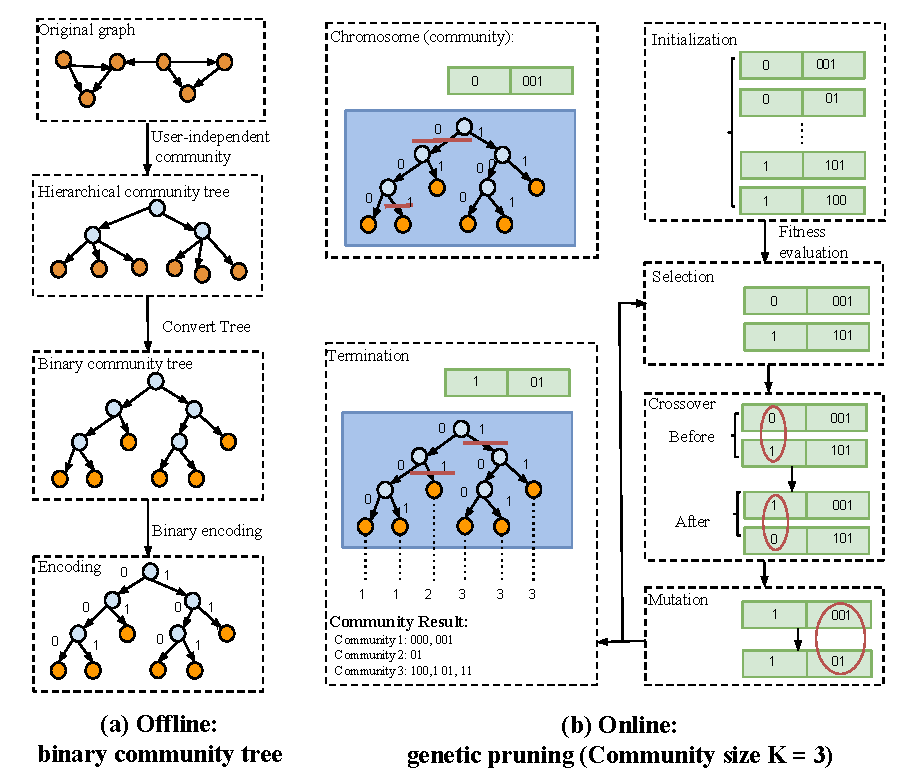
\includegraphics[width=1.0\columnwidth]{img/chapter3/4.pdf}
	%  \vspace{-3em}
	\caption{The framework of gPCD model. (a) refers to the offline construction step on the original graph and (b) refers to the online genetic pruning step to generate personalized communities.} 
	\label{fig:pipeline}
	%  \vspace{-1em} 
\end{figure}
In \textit{$T_{c}(N^{c},L^{c})$}, each parent node can have multiple child nodes which can be regarded as a community partition on the parent node. For instance, a node $N_{k}^{c} \in N^{c}$ from $T_{c}(N^{c},L^{c})$ represents a community of vertices.  Its $m$ child nodes $\{N_{k_{1}}^{c},N_{k_{2}}^{c},...,N_{k_{m}}^{c}\}$ represent $m$ sub-communities of vertices from $G(V,E)$ where we have $	\bigcap_{i=1}^{m} N_{k_{i}}^{c} = \varnothing$ and  $	\bigcup_{i=1}^{m} N_{k_{i}}^{c} =  N_{k}^{c}$.  



In order to achieve an efficient personalized community detection in the following online step, I convert the hierarchical community tree \textit{$T_{c}(N^{c},L^{c})$} to a binary community tree \textit{$T_{b}(N^{b},L^{b})$} for index. Specifically, for $m$ child nodes of a parent node $N_{k}^{c}$, a bottom-up approach is proposed to merge a selected pair of sibling nodes as a new node in an iterative manner. The approach runs until all $m$ child nodes merged together to form the parent node $N_{k}^{c}$. To avoid an unbalanced tree where small communities are always left to merge with huge communities in the end, I first select the node with the smallest community size among all sibling nodes in each merging step. It is merged with its sibling node with the largest normalized linked weight (Please refer to Figure \ref{fig:pipeline}(a)). The normalized linked weight function $w(\cdot)$ between  two nodes $N_{i}^{c}$ and $N_{j}^{c}$ is defined as:
\begin{equation} 
\textit{$w(N_{i}^{c},N_{j}^{c})$} =\frac{\textit{$N_{i}^{c}\odot N_{j}^{c}$}-\frac{\mathcal{D}(N_{i}^{c})\cdot \mathcal{D}(N_{j}^{c})}{2|E|} }{\textit{$| N_{i}^{c}||N_{j}^{c}|$}} 
\end{equation} 
where \textit{$N_{i}^{c}\odot N_{j}^{c}$} denotes the number of edges linked between vertices in node \textit{$N_{i}^{c}$} and \textit{$N_{j}^{c}$}, which can be interpreted as the linkage strength between them; \textit{$|N_{i}^{c}|$} is the number of vertices inside node \textit{$N_{i}^{c}$}; \textit{$\mathcal{D}(N_{i}^{c})$} is the out-degree of node \textit{$N_{i}^{c}$} (the total number of edges linked to other nodes) and \textit{$|E|$} is the total number of edges in the original graph $G(V,E)$ . $\frac{\mathcal{D}(N_{i}^{c})\cdot \mathcal{D}(N_{j}^{c})}{2|E|} $ denotes the random linkage strength between node \textit{$N_{i}^{c}$} and \textit{$N_{j}^{c}$}. The \textit{$w(\cdot)$} function calculates how much that two nodes are better connected beyond random connection and is normalized by node size. Given the node $N_{i}^{c}$ with the smallest community size and all its sibling node set $S$, The merging step can be formulated as:
\begin{equation}  
\begin{aligned} 
& N_{j}^{c} \Leftarrow \argmax_{N_{j}^{c} \in S}w(N_{i}^{c},N_{j}^{c})\\
& N_{*}^{c} = N_{i}^{c}\bigcup N_{j}^{c}
\end{aligned}
\end{equation}
The bottom-up process will stop until all child nodes are merged together to form the parent node. In the end, the hierarchical community tree \textit{$T_{c}(N^{c},L^{c})$} is fully converted to a binary community tree \textit{$T_{b}(N^{b},L^{b})$} with user-independent community information.  The node size $|N^{b}|$ as well as the link size $|L^{b}|$  in \textit{$T_{b}(N^{b},L^{b})$} is at most $2|V|$ which is smaller than the size of original graph $G(V,E)$. If I consider to form the binary community tree with only $k$ levels, the size of \textit{$T_{b}(N^{b},L^{b})$} can be even smaller. 

\begin{table}[h]
	%\scriptsize
	%	\small
	\centering
	
	\begin{tabular}{|p{3cm}|p{11cm}|} 
		\hline
		\textbf{Notations} & \textbf{Descriptions} \\ \hline
		$G(V,E)$ & Original graph $G$ with vertex set $V$ and edge set $E$ \\ \hline
		\textit{$T_{c}(N^{c},L^{c})$} & The hierarchical community tree generated from graph $G(V,E)$ with node set $N^{c}$ and link set $L^{c}$. Each node  $N^{c}_{k} \in N^{c}$ denotes a group of vertices belonging to $V$. \\\hline
		\textit{$T_{b}(N^{b},L^{b})$} & The binary community tree reconstructed from \textit{$T_{c}(N^{c},L^{c})$}. Each node $N^{b}_{k} \in N^{b}$ denotes a group of vertices belonging to $V$. \\ \hline
		$B$ & The binary codebook for \textit{$T_{b}(N^{b},L^{b})$}. Particularly, $B_{k} \in B$ denotes the binary code of both $N_{k}^{b} \in N^{b}$ and $L_{k}^{b}\in L^{b}$ where $L_{k}^{b}$ is the link points to node $N_{k}^{b}$.
		\\ \hline
	\end{tabular}
	\caption{Commonly used notations in gPCD model}
	\label{tab:notation}
	\vspace{-1em}
\end{table} 


For running time analysis, calculating normalized linked weight takes constant time. In each merging step, node pair selection takes linear time. Therefore, in the worst case, the time complexity of binary community tree construction is $O(|V|^2)$ where the depth of the hierarchical community tree $T_{c}(N^{c},L^{c})$ is 1 and each vertex in $G(V,E)$ forms a single-vertex community.

To encode the nodes and links on $T_{b}(N^{b},L^{b})$ as binary code, the root node is encoded as `null' first. For a parent node \textit{$N_{k}^{b}$} with its left child node \textit{$N^{b}_{k_{l}}$} and right child node \textit{$N^{b}_{k_{r}}$}, the binary code of a child node and the related link defined in the Notation Table \ref{tab:notation} is calculated as: 

\begin{eqnarray}\text{$B_{k_{i}}$}=
\begin{cases}
\text{$B_{k}$}+``0", & i = ``l"\cr 
\text{$B_{k}$}+``1", & i = ``r"
\end{cases}
\end{eqnarray} 

For instance, if the node \textit{$N_{k}^{b}$} is with binary code ``$00$," its left child node's binary code is ``$000$" while the right child node's binary code is ``$001$." The link \textit{$L_{k}^{b}$} that points to \textit{$N_{k}^{b}$} also has the binary code ``$00$". 

\subsection{Community and User Need Representation} \label{sc:c3_representation}

Node2vec \cite{grover2016node2vec} helps to learn fixed-length embeddings for both user need and communities. It simulates random walks on the graph $G(V,E)$ and learns the vertex embedding by optimizing the sequential relationships from random walk paths. In the end, each vertex $V_{k}$ in graph $G(V,E)$ has a vector representation as $\vec{V_k}$. Each node $N_{k}^{b}$ on the binary community tree \textit{$T_{b}(N^{b},L^{b})$} refers to a vertex community $C_{k}$ in the graph $G(V,E)$. Its representation $\vec{C_{k}}$ is calculated as the averaged embedding of all vertices inside the community. In the end, the binary community tree \textit{$T_{b}(N^{b},L^{b})$} represents the hierarchical community partition of Graph $G(V,E)$. Each node \textit{$N_{k}^{b}$} on the tree is indexed with three attributes: a group of vertices from graph $G(V,E)$, a binary code \textit{$B_{k}$}, and an embedding representation \textit{$\vec{C}_{k}$}.

On the other hand, User need (query) $I$ can also be represented by a combination of $t$ different vertices $\{V_1, V_2... V_t\}$ in the graph $G(V,E)$. In this study, two different scenarios for user need representation are offered:

\textbf{Vertex-based Query}. User need can be directly represented by the vertices based on the generation probability $P(V_k|I)$ between them. Hence the user need representation $\vec{I}$ is calculated as:

\begin{equation}
\vec{I} = \sum_{k=1}^{t} P(V_k|I) \cdot \vec{V_k} 
\end{equation} 
For instance, in a music sharing network, each vertex $V_k$ denotes a music and a user listing history can be used to reflect the user need $I$. $P(V_k|I)$ therefore can be regarded as the probability that a music being listened by the user. 

\textbf{Text-based Query}. Under this scenario, user need $I$ is represented as a text query, and each vertex $V_{k}$ in the graph $G(V,E)$ also contains textual content. From language model viewpoint, each vertex importance weight is the query likelihood $P(I|V_k)$, and the user need can is the weighted average of vertex embedding: 

\begin{equation}
\vec{I} = \frac{\sum_{k=1}^{t} P(I|V_k) \cdot \vec{V_k}}{\sum_{k=1}^{t} P(I|V_k)}
\end{equation}

In either case, user need is conceptualized as an embedding with the same dimension as the node embeddings on the binary community tree. It enables very efficient online personalized community detection in later steps. And running Node2vec takes most of the time in this step.   

\subsection{Online Genetic Pruning} \label{sc:c3_online}

The whole process, as the Figure \ref{fig:pipeline} shows, is to generate communities by pruning the constructed binary community tree. After each cut on a link, the original tree  will be separated into two sub-trees. After a specific number of cuts to the links on the tree, a fixed number of communities with different resolutions are detected.  By applying genetic selection, crossover, and mutation steps, the model converges to the optimized solution efficiently with a clear-defined fitness function. The details are shown in the following paragraphs.

\subsubsection{Genetic Representation} 

A chromosome is formed by a set of genes \{$g_{1},g_{2},...,g_{K-1}$\}, and each gene $g_{i}$ holds a cut link $L_{i}^{b}$ in the binary community tree \text{$T_{b}(N^{b},L^{b})$}. Since communities can be created by cutting links on the offline tree, a chromosome can be represented as a generated community partition of the original graph $G(V,E)$ in this way. 
To constrain a chromosome so that it can be decoded to a fixed number of communities, four \textbf{Cutting Rules} are necessarily to be applied: 
\begin{itemize} %\itemsep0em
	\item \textbf{ Rule 1}: If a link $L_{i}^{b}$ is picked to cut on the binary community tree \text{$T_{b}(N^{b},L^{b})$}, its pointing node $N_{i}^{b}$ will be retrieved and all the vertices within it form a community. 
	\item \textbf{ Rule 2}: If a link {$L_{i}^{b}$} and its ancestor link {$L_{j}^{b}$} are stored in the same chromosome, all vertices in {$L_{i}^{b}$}'s related node {$N_{i}^{b}$} are a subset of vertices in {$L_{j}^{b}$}'s related node {$N_{j}^{b}$}. In this case, the two cut links generate two communities where community $C_{i}$ is all vertices in $ N_{i}^{b}$ and community $C_{j}$ is the remaining vertices in $ N_{j}^{b}$ but not in $ N_{i}^{b}$. It can be formulated as   $C_{i} = \bigcup_{k}\{V_{k}|(V_{k}\in N_{i}^{b})\}$ and community $C_{j} = \bigcup_{k}\{V_{k}|(V_{k}\in N_{j}^{b}) \cap (V_{k}\notin N_{i}^{b})\}$.  
	\item \textbf{ Rule 3}: Sibling links can't be stored in the same chromosome, and it is not allowed to store duplicated links in a chromosome.
	\item \textbf{ Rule 4}: The depth's upper bound is set to be $d$, which means all eligible cut links should be located in the first $d$ depth on the binary community tree. It avoids to generate super tiny communities and hugely reduces the genetic searching scope on cut links.
\end{itemize} 

By applying the cutting rules to the online pruning process, I ensure a $K$ community partition can be retrieved from a chromosome with $K-1$ cut links.  


\subsubsection{Initialization}

Initially, the model generates a given number $P$  chromosomes as the seed ``chromosome population". And each iteration in the genetic approach breeds a new ``generation'' of chromosome population. In order to ensure a chromosome is an encoder of a $K$ community partition, $K-1$ links will be randomly picked (on the binary community tree) following the cutting rules and stored in the related genes of a chromosome. 

\subsubsection{Fitness Function} 

As each chromosome can be decoded as a community partition, it is important to measure the quality of each generated chromosome (how well the generated communities can satisfy user need). The measurement is hosted in a fitness function. 


In the proposed model, the fitness function simulates the user searching behavior on the graph given the community partition. For instance, a user can be more likely to pick the most relevant communities while avoiding the redundant information already selected. With the help of the offline step, the relevance score of node $N_{i}^{b}$ (community $C_{i}$) towards user need $I$ can be calculated with the cosine similarity $cos(\vec{I},\vec{C_{i}})$, and the information redundancy can be $\sum_{C_{j} \in S_c}cos(\vec{C_{j}},\vec{C_{i}})$ where $S_{c}$ is the set of communities that the user have already picked from the communities decoded from the target chromosome. Following this, I use a greedy selection approach to iteratively rank and pick communities given a chromosome (community partition) until all communities are picked: 

\begin{equation}  \argmax_{C_{i}}\lambda \cdot cos(\vec{I},\vec{C_{i}})-(1-\lambda)\cdot \frac{\sum_{C_{j} \in S_c}^{ }cos( \vec{C_j},\vec{C_{i}})}{|S_c|}
\end{equation} 

where $C_i$ is the candidate community to be picked and $|S_c|$ is the number of communities already been picked. $\lambda$ is a parameter controls  whether user prefers to obtain new useful information or to avoid redundant information.  

For chromosome quality evaluation, a query-generated vertex ranking list $l_{q}$ is first created by retrieving top $n$ vertices relevant to the query (user need) with the largest cosine similarities on embeddings of graph $G(V,E)$. I store the top $n$ vertex ranking label $R(l_{q})=\{1,2,...,n\}$ as the pseudo ground truth. On the other hand, given the $k_{th}$ chromosome $ch_k$ in the current chromosome generation, I can also retrieve the community-generated ranking of each vertex $V_{k} \in l_{q}$ from the sequentially selected communities decoded by the chromosome. I assign the ranking label on each vertex $V_{k}$ based on the following formula:
\begin{equation}
\sum_{V_{j} \in l_{q}}\Phi(\delta(V_{j}) < \delta(V_{k})) + 1
\end{equation} 

$V_{j}$ refers to all vertices in $l_{q}$. $\delta(V_{j})$ shows the ranking (selection sequence) of the community which $V_{j}$ belongs to. $\Phi$ is a binary operator to determine whether $V_{j}$ satisfy the condition $\delta(V_{j}) < \delta(V_{q})$. This formula helps to construct the community-generated ranking label $R(l_c)$. For instance, when $n=3$, I have a query-generated ranking list $l_q = \{V_1,V_2,V_3\}$ and its related ranking label $R(l_q) = \{1,2,3\}$. Given a chromosome where the community of $V_1$ and $V_2$ is the same and selected before $V_3$, I can generate the related community ranking label $R(l_c) = \{1,1,3\}$ with the same vertex sequence of $l_q$.

Then, I define the fitness function $f(\cdot)$ to evaluate the chromosome $ch_{k}$. As I have the query-generated ranking label $R(l_{q})$ (ground truth) and community-generated ranking label $R(l_{c})$ from $ch_{k}$, I calculate their Kendall's $\tau$  correlation coefficient  as the fitness score $f(ch_k)$ of chromosome $ch_k$ where higher score means the chromosome $ch_{k}$ can  generate better personalized communities to meet with user need. 

\begin{equation}
\textit{$f(ch_{k})$} = 1-\frac{\sum_{i=1}^{n} R(l_{ci})\cdot R(l_{qi})}{\sum_{i=1}^{n} R(l_{ci})^2\cdot \sum_{i=1}^{n}R(l_{qi})^2}
\end{equation} 
where $R(l_{ci})$ is the $i_{th}$ vertex ranking in community-generated ranking label $R(l_{c})$ and $R(l_{qi})$ is the $i_{th}$ vertex ranking in query-generated ranking label $R(l_{q})$. Kendall's $\tau$ is a widely used metric to evaluate the correlation between two lists where higher score means stronger correlation. Thus, higher fitness score reflects that the generated community ranking $R(l_{c})$ can better meet with user need $R(l_{q})$. 

Moreover, it is clear that the fitness function aims to separate all top $n$ vertices in different communities to get the optimal case. It matches the research goal to generate high resolution communities on vertices which are more relevant to user need. As the number of community is a given number $K$, it also leads to a coarser manner partition on the remaining less relevant vertices. On the other hand, the binary community tree $T_{b}(N^{b},L^{b})$ and the Cutting Rule 4 naturally preserve the community structure and unite the most relevant vertices in the same community. Hence the whole genetic approach is a gambling process. The final chromosome result is the equilibrium case to detect communities both contain graph topological structure and meet with user need.


\subsubsection{Selection}

I select the superior chromosomes from current chromosome population based on their fitness scores. The probability that the $k_{th}$ chromosome $ch_k$ is picked can be calculated via the Softmax normalization function $p(ch_{i}) = \frac{exp(f(ch_{k}))}{\sum_{i=1}^{P}exp(f(ch_{i}))}$. Then, the Fitness Proportionate Selection method is applied to randomly select $P$ chromosomes into chromosome pairs based on probability distribution. In order to enhance optimization efficiency, I also use elitism selection to ensure the best chromosome in the current generation will always be selected to the next generation. 

\subsubsection{Crossover} 

To reach global optimum community partition efficiently, given a pair of chromosomes, the crossover operation can randomly exchange part of the genes in both chromosomes to produce a new pair of chromosomes with a certain crossover rate.

In order to make sure that the newly generated chromosomes meet the cutting rules, an \textbf{Exchange Rule} is defined to restrict gene exchange: If gene \textit{$g$} contains link $L^{b}_{g}$, \textit{$g$} can't do crossover process with genes that contain either link $L^{b}_{g}$ or its sibling link $L^{b'}_{g}$. This rule can help avoid having duplicated links or sibling links stored together in the newly generated chromosome (To satisfy Cutting rule 3). 

After \textit{$m$} random numbers are selected from \{$1,2,...,K-1$\} as exchanged gene position indexes, genes located in the chosen positions of two chromosomes will exchange the stored link restricted by the Exchange Rule.
\subsubsection{Mutation} 
Mutation operation is applied to avoid local optimization. If a chromosome is chosen to mutate, a gene within the chromosome will be randomly picked, and its stored link will be changed to another link restricted by the Exchange Rules. An example is illustrated in Figure \ref{fig:pipeline}(b) where the link stored in the second gene is changed from ``001'' to ``01''. 

\subsubsection{Termination}

After $T$ iterations, the whole process stops and the current best chromosome is retrieved as the final result. Choosing the number of $T$ is dependent on the task. In order to decode the final chromosome to the related community partition, all genes in the chromosome are sorted in an ascending order based on the binary code of their stored cut link. Vertices whose binary codes start with the same cut link's binary code will be assigned to the same community label. And its later assigned community label can overwrite the previous assigned community label. For instance, if there are a vertex with binary code ``0011'' and two cut links with binary code ``00'' and ``001'', the vertex will be assigned to a community label ``00'' first, and its community label is overwritten by ``001'' afterwards. The Termination step in Figure \ref{fig:pipeline}(b) also illustrates a vivid example. In this way, the binary code of the binary community tree can help to decode the final chromosome into communities in an efficient way. 
 

\subsection{Distributed gPCD} \label{sc:c3_distributed}
 
To enhance the online step efficiency, a MapReduce framework is utilized to enable the distributed genetic evolution. Figure \ref{fig:distributed} depicts the personalized community detection under a MapReduce framework. The chromosome collection is either originally initialized from binary community tree or obtained from the last generation. It contains the whole chromosome population in the central depository. In its first ``Splitter'' process, all chromosomes are split into $M$ groups based on their hash values and sent out to related $M$  Mappers to calculate the ``Fitness'' scores. In the same Mapper, after all chromosomes are assigned fitness scores, based on their scores, a Combiner groups all chromosomes together and random select equal number of chromosomes with duplicated as the ``Selection'' step. All the selected chromosomes are sent to $R$ reducers (I set $R = M$ arbitrarily in order to better represent time complexity) to form pairs for the ``Crossover'' and  ``Mutation'' step, calculate new chromosome offsprings for the next generation and store them back to the central repository. 
 
\begin{figure}  
	% \advance\leftskip-4cm 
	\center
	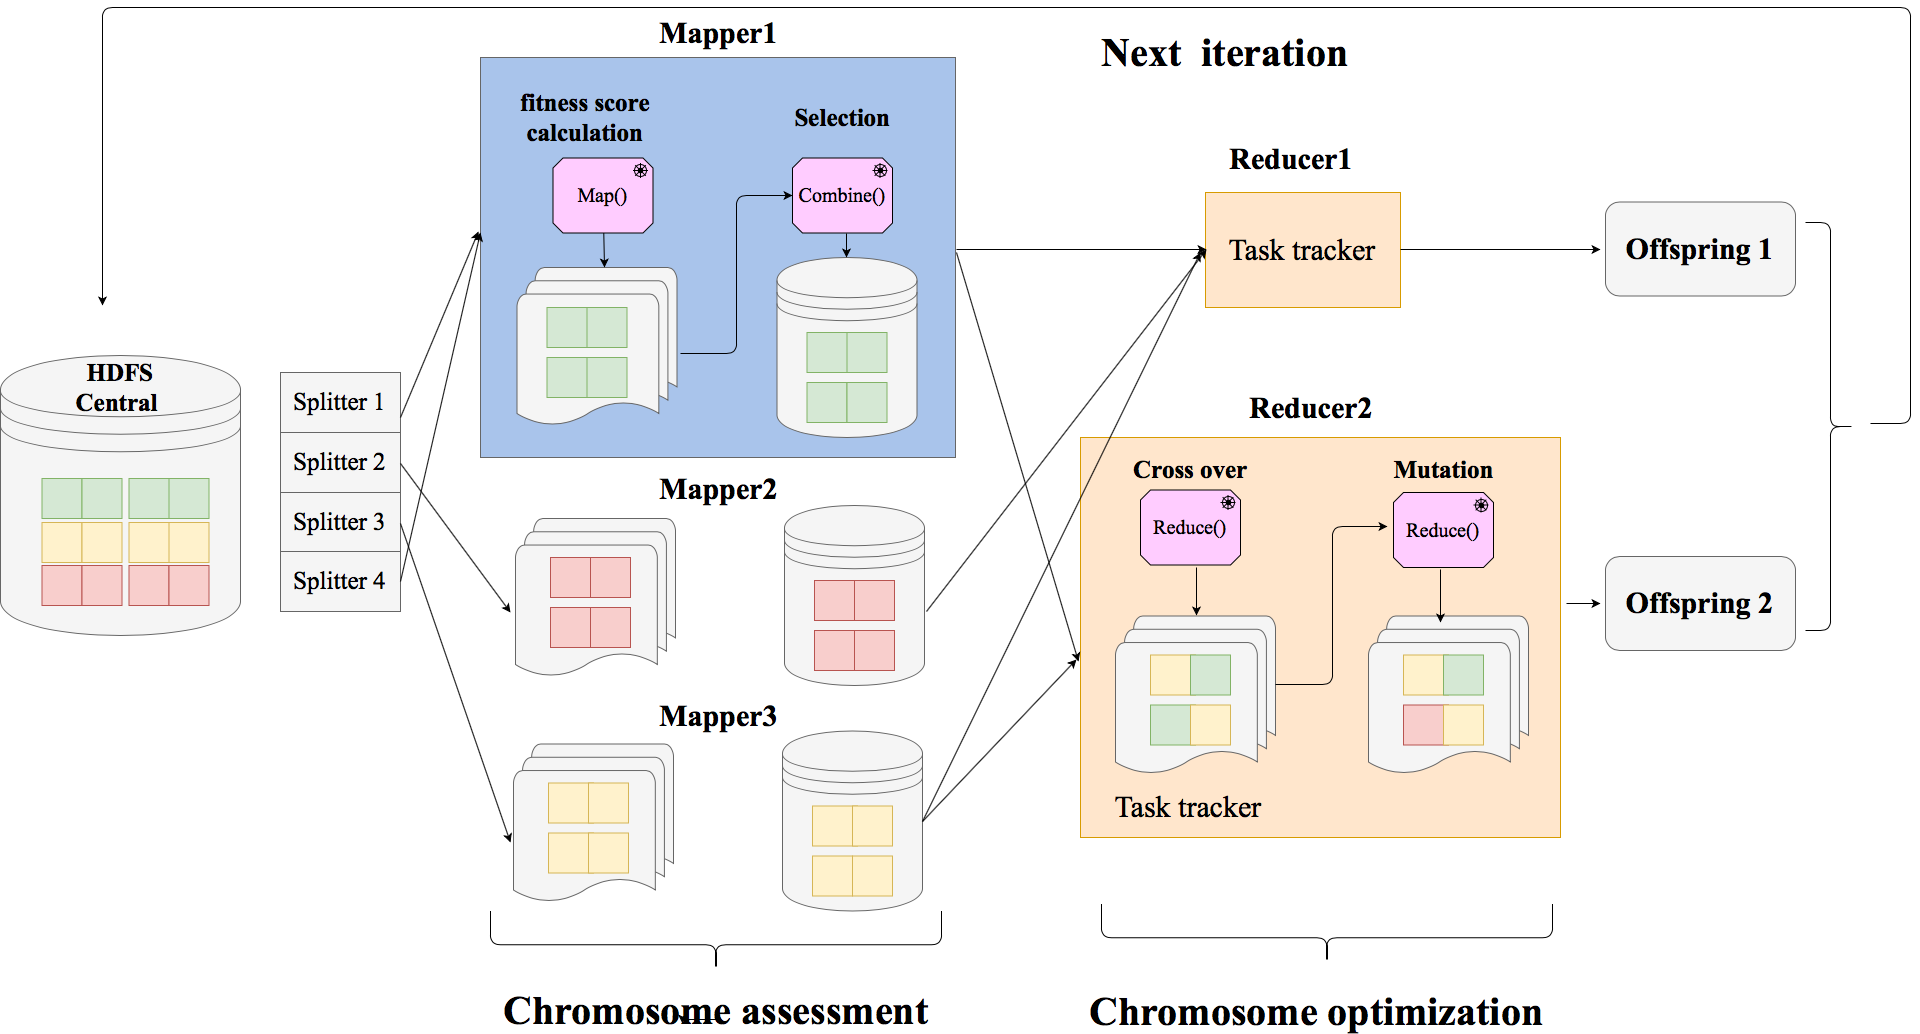
\includegraphics[width=1\columnwidth]{img/chapter3/parallel.png}
	%  \vspace{-3em}
	\caption{Online parallel computing process on Hadoop Distributed File System (HDFS)}
	%  \vspace{-1em} 
	\label{fig:distributed}
\end{figure}

The complexity of the proposed algorithm is $O(2^dKP)$ without parallel computing and $O(\frac{2^dKP}{M})$ with  parallel computing, where $d$ denotes the upper bound where the cut links are restricted in the top $d$ depth of the binary community tree $T_{b}(N^{b},L^{b})$; $K$ denotes the community number; $P$ denotes the initialized population size of the genetic algorithm and $M$ denotes the number of Mappers/Reducers in parallel environment. As all the parameters are considerably small (compared with the node/edge size in the original graph), the whole process runs very fast to retrieve the final community partition.
\section{Experiments}

\subsection{Datasets} 
\subsubsection{Datasets Description} 

 
\begin{table}[h]
	%\scriptsize
	\centering
	
	\begin{tabular}{|c|c|c|c|c|} 
		\hline
		\multirow{2}{*}{\textbf{Dataset}}  &\multicolumn{2}{c|}{\textbf{Node description }} & \multicolumn{2}{c|}{\textbf{Edge description}}\\ \cline{2-5}%\cmidrule(lr){4-5}
		& Type & Size & Type & Size \\ \hline
		Scholarly & paper & 166,170 & citation &750,181\\ \hline
		Music & song & 145,203 & co-listening &1,172,525
		\\ \hline
	\end{tabular}
	\caption{Dataset Description}
	\label{tab:c3_dataset}
\end{table} 

Table \ref{tab:c3_dataset} shows the statistics of the two datasets.  The scholarly graph is unweighted and directed, while the music graph is a weighted and undirected.

\textbf{Scholarly Graph:} It contains academic publications with metadata extracted from ACM Digital Library. From the dataset, I build the experimental graph via paper citation relationship. Each vertex in the graph represents a paper, and if a paper cites another paper, there will be an edge linking the two. My model aims to detect personalized communities on the scholarly graph for authors. For each author in the dataset, I represent his/her need in two ways: their previous publications (text-based query) and cited paper history (vertex-based query).  

\textbf{Music Graph:} It contains user listening histories and user-generated playlists from an online music streaming service, Xiami. I create a music graph with songs as the vertices and co-listening relationship as the edges. If two songs appear in the same user's listening history, there will be an edge linking them two. For users in the music dataset, I represent their music tastes (user need) from the songs in their listening history.  

\subsubsection{Ground Truth Construction}

The ground truth for the two datasets are generated based on each user's publishing/ citing/ listening history:

For the scholarly dataset, the references of 112 random sampled papers are manually annotated from their literature reviews where authors summarize previous works. Different paragraphs (or sub-sections) in the literature review typically focus on separate but coherent topics while the same paragraph talks about the same topic. Based on this assumption, the papers cited in the same paragraph/sub-section naturally form a community with high resolution. To ensure each paper's cited papers form enough communities and each community contains enough papers, only papers with no fewer than three topics and all of whose communities have at least five papers are kept. After applying all these filters, 101 papers are left for evaluation.  

For the music dataset, each user has several self-generated playlists. The songs in each playlist should contain a coherent theme. To avoid the playlists sharing mutually exclusive themes with other playlists, a Jaccard similarity check is applied on any pair of playlists created by the same user. If a user has at least two highly correlated playlists (Jaccard coefficient between them is above 0.5), I remove one of the playlists. Each playlist forms a separate community. Furthermore, to ensure the number of playlist and playlist size are both large enough, only users with at least three playlists and each playlist contains at least five songs are kept. In the end, there are 117 users who meet the above criteria. 

In this paper, as all communities constructed in the ground truth are relevant communities with high resolution for users, my task is generating personalized communities to reconstruct the ground truth on two different datasets with vertex- and text-based user need. 

\subsection{Settings}

\subsubsection{Metrics \& Parameter Settings}

F1-score (F1), Rand index (Rand), Jaccard index (Jaccard) and running time are reported as the evaluation metrics in this paper. Based on empirical studies, population size $P$ is 100. Crossover rate is 95\%. Mutation rate is 1\%. The maximum depth of binary community tree $d$ is 10. The number of iteration $T$ is 30. User searching preference $\lambda$ is 0.6. Community size $K$ is 50. The number of Mappers/ Reducers for parallelization $M$ is 50. The number of top vertices to construct pseudo ground truth $n$ is 10. Parameters in Infomap and Node2vec are both the default settings in their original papers. 

\subsubsection{Baselines} 

Considering both efficacy and efficiency, I select eight widely used user-independent community detection models. Ideally, to achieve personalized community detection, user-independent models should run on each user separately by assigning higher weights on user related edges. Thus, their time complexity should be only compared with my online step time complexity as my offline step is independent with user numbers. In this paper, to run baselines within acceptable time, I report their user-independent community results as the average performance. 

\begin{itemize}
	\item \textbf{Spinglass} \cite{eaton2012spin}: Spinglass  constructs communities by minimizing the Hamiltonian score on signed graphs.\footnote{https://github.com/antoine-lizee/SG}
	\item \textbf{Fast Greedy} (FG) \cite{clauset2004finding}: Fast Greedy  is a greedy search method to get the maximized modularity for community detection.\footnote{https://github.com/kjahan/community}
	\item \textbf{Louvain} \cite{blondel2008fast}: Louvain  is an agglomerative method to construct communities in a bottom-up manner guided by modularity.\footnote{https://github.com/taynaud/python-louvain}
	\item \textbf{Walktrap} \cite{pons2005computing}: Walktrap detects communities based on the fact that a random walker tends to be trapped in dense part of a network.\footnote{https://www-complexnetworks.lip6.fr/~latapy/PP/walktrap.html}
	\item \textbf{Infomap} \cite{rosvall2011multilevel}: Infomap generates communities by simulating a random walker wandering on the graph and indexing the description length of his random walk path via multilevel codebooks.\footnote{http://www.mapequation.org/code.html}
	\item \textbf{Bigclam} \cite{yang2013overlapping}: Bigclam generates overlapping communities via a non-negative matrix factorization approach.\footnote{https://github.com/snap-stanford/snap/tree/master/examples/bigclam}
	\item \textbf{DeepWalk} \cite{perozzi2014deepwalk}: DeepWalk generates node embeddings via random walks and utilizes K-means on node embeddings to detect communitis.\footnote{https://github.com/phanein/deepwalk/tree/master/deepwalk}
	\item \textbf{Node2vec} \cite{grover2016node2vec}: Node2vec is an extended version of DeepWalk with a refined random walk strategy.\footnote{https://github.com/aditya-grover/node2vec}
\end{itemize}


\section{Discussion} 
\subsection{Evaluation Results}  \

There are two scenarios to construct user need. For the scholarly graph, including a citation (vertex-based query) model and a keyword (text-based query) model. In the citation model, for each user, we first extract all the papers he/she cited before, then use their centroid embedding as user need vector  $\vec{I}$. In the keyword model, for each user (author), I first extract all keywords he/she used in all previous papers to form a text query. Then I retrieve the top 100 relevant papers given the query based on probability language model with Dirichlet smoothing. Finally, I average those retrieved papers' vectors as the user need vector $\vec{I}$.

\begin{table}[h]
	% 	\scriptsize
%	\small
	 \centering
	%\vspace{-3em}
	
%	\renewcommand{\tabcolsep}{3.0pt} 
%	\renewcommand\arraystretch{0.0}
	\begin{tabular}{|c|c|c|c|c|c|c|} 
		\hline
		\multirow{2}{*}{\textbf{Model}} & \multicolumn{3}{c|}{\textbf{Scholarly Graph}} 	&\multicolumn{3}{c|}{\textbf{Music Graph}}\\
		\cline{2-7}%\cmidrule(lr){2-7}
		& F1 & Rand	& Jaccard	& F1 & Rand	& Jaccard\\  \hline
		Spinglass&0.4294 & 0.4149 &0.3593 & 0.4282 & 0.5317& 0.2823 \\ 
		FG& 0.4290 & 0.3852& 0.3735 &0.4645&0.4100& 0.3070 \\ 
		Louvain&0.4417 & 0.4546& 0.3627&0.1832 &0.4201 & 0.1174 \\ 
		Walktrap& 0.4304 & 0.3777 & 0.3777&0.3999 & 0.3507& 0.3490 \\
		Infomap&0.4436 & 0.4165& 0.3606& 0.2147 & \textbf{0.6074} &0.1344\\ 
		Bigclam& 0.2314  & 0.2572 & 0.1348 & 0.1499  & 0.2078  & 0.1227 \\
		DeepWalk&0.3904 & 0.3237 & 0.3234&0.3535& 0.3253& 0.3001 \\ 
		Node2vec & 0.4001 & 0.3472 & 0.3433&0.4122 & 0.4101& 0.3087 \\  \hline
		gPCD-Citation&$\textbf{0.5351}^{*}$ & $\textbf{0.4551}^{*}$& $\textbf{0.4086}^{*}$ &-	&-	& -\\
		gPCD-Keyword&0.5069 & 0.4114& 0.3708 &-	&-	& - \\
		gPCD-Listening&-	&-	& - &$\textbf{0.5188}^{*} $& 0.5865& $\textbf{0.3550}^{*} $\\ 
	\hline
	\end{tabular}
	\begin{tablenotes}
		\item[] \begin{footnotesize}
			Note: ``*'' means the p-value through a pairwise t-test is smaller than 0.001.
		\end{footnotesize}
	\end{tablenotes}
	\caption{Personalized Community Evaluation on gPCD and Baselines. }
	\label{tab:community}
\end{table}


For the music task, text information is not available. The centroid embedding of the songs listened to by a target user are taken as user need.

\textbf{Community Accuracy}: I compare the average performance of my model on all testing users with baselines. Table \ref{tab:community} shows the detailed metrics. When running on the Scholarly graph, both Citation model and Keyword model can achieve around 10\% increase on F1-score compared with all baselines. Citation model also performs the best in Rand Index and Jaccard Index. For Music graph, my Listening model also has a significant improvement on F1-score and Jaccard Index. Although it has similar performance on Rand Index compared with Infomap, I believe my model in fact works much better due to the Infomap's poor performance on the rest two metrics. Moreover, I apply pairwise t-tests for all metrics on all testing users. All metrics' p-values in Citation model and the p-values of F1-score and Jaccard Index in Listening model are all smaller than 0.001, which means the improvements of my model performance are significant compared with baselines.


\textbf{Running Time Comparison}: Table \ref{tab:complexity} shows both the theoretical time complexity and real running time. To represent baseline algorithms' time complexity, ``$V$" refers to the vertex set and ``$E$" refers to the edge set in the graph $G(V,E)$. For some models (FG, Walktrap, and Infomap.), their specific time complexities are officially mentioned in the original papers. The time complexity of Louvain and Bigclam are roughly estimated in the original papers as well but those papers don't mention specific numbers. For Spinglass, DeepWalk and Node2vec, I can't find the exact time complexity in existing studies. Hence in this paper, I arbitrarily assign labels based on the their real running speed. Considering the running time, all the baseline algorithms run relatively fast except for the Spinglass algorithm. However, compared with all other models, the distributed gPCD always performs the fastest. Its real running time of is less than one-tenth of the fastest baseline's running time. 

\begin{table}[h]
	% 	\scriptsize
%	\small
	\centering
	%\vspace{-3em}
%	\renewcommand{\tabcolsep}{2pt} 
%	\renewcommand\arraystretch{0.0}
	\begin{tabular}{|c|c|c|c|} 
		\hline
		\textbf{Model}& \textbf{Time Complexity} & \textbf{Scholarly Graph} (s)	& \textbf{Music Graph} (s) \\ \hline
		Spinglass& very slow &12548.68	& 10372.17 \\ 
		FG& $O(|V|log^2|V|)$&280.60	& 272.34 \\ 
		Louvain& linear&80.01	&63.02 \\ 
		Walktrap&$O(|V|^2log|V|)$& 638.44	& 503.24 \\
		Infomap&$O(|V|(|V|+|E|))$ &501.79	&425.63 \\ 
		Bigclam&linear &57.01 	& 112.43 \\ 
		DeepWalk& fast&720.56	& 688.32 \\ 
		Node2vec& slow&	3508.44&3100.12 \\ 
		gPCD&$O(\frac{2^dKP}{M})$ &\textbf{5.25} &\textbf{6.50} \\ 
		\hline
	\end{tabular}
	\caption{Running time analysis on gPCD and all baselines in seconds (s).}
	\label{tab:complexity}
%	\vspace{-3em}
\end{table}

\subsection{Parameter Analysis}  
\begin{figure}
	\subfloat[Depth $d$ in Citation model]{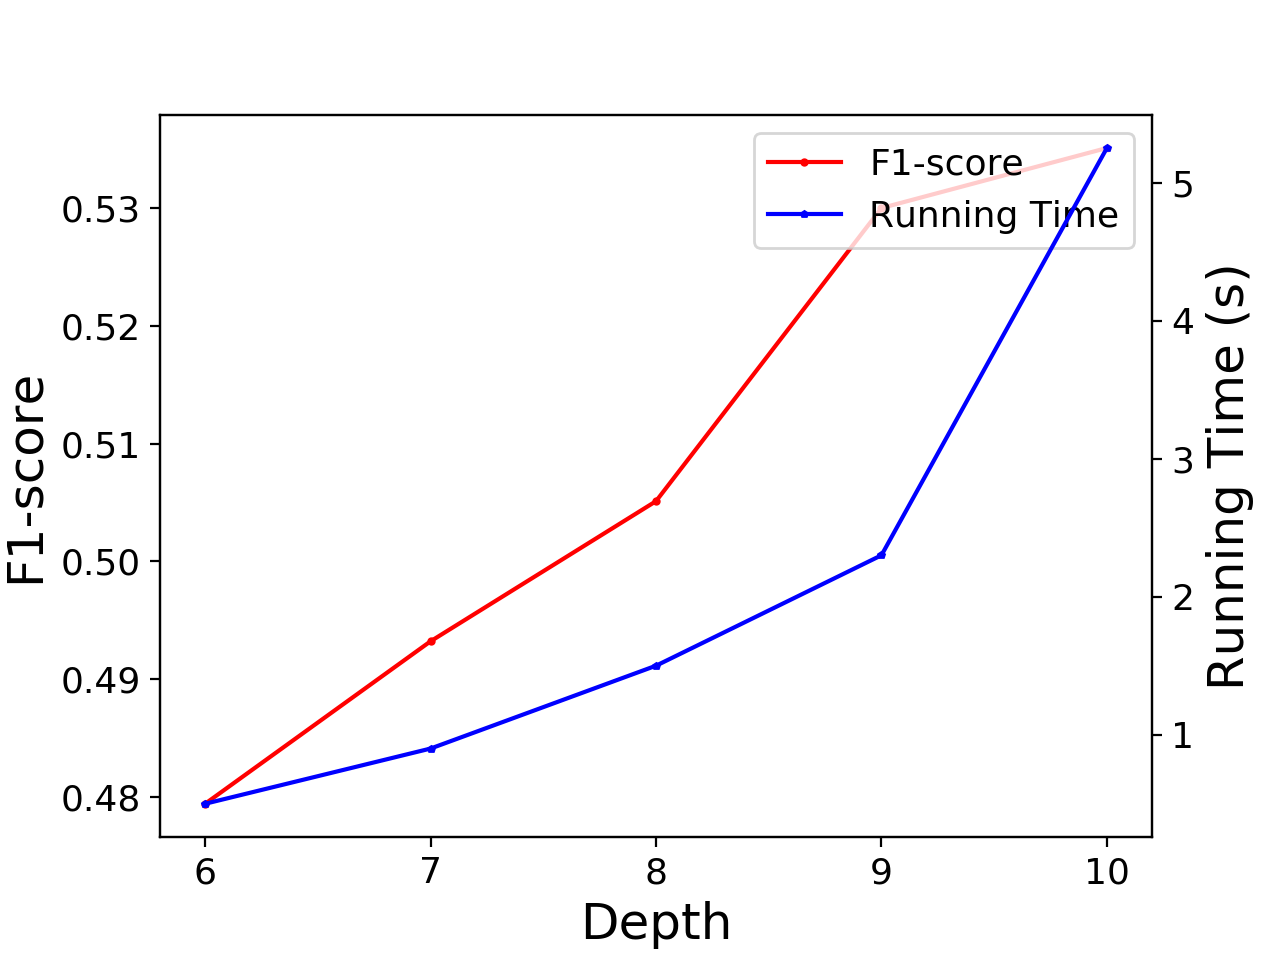
\includegraphics[width = 0.33\columnwidth]{img/chapter3/citation.png}}
	\subfloat[Depth $d$  in Keyword model]{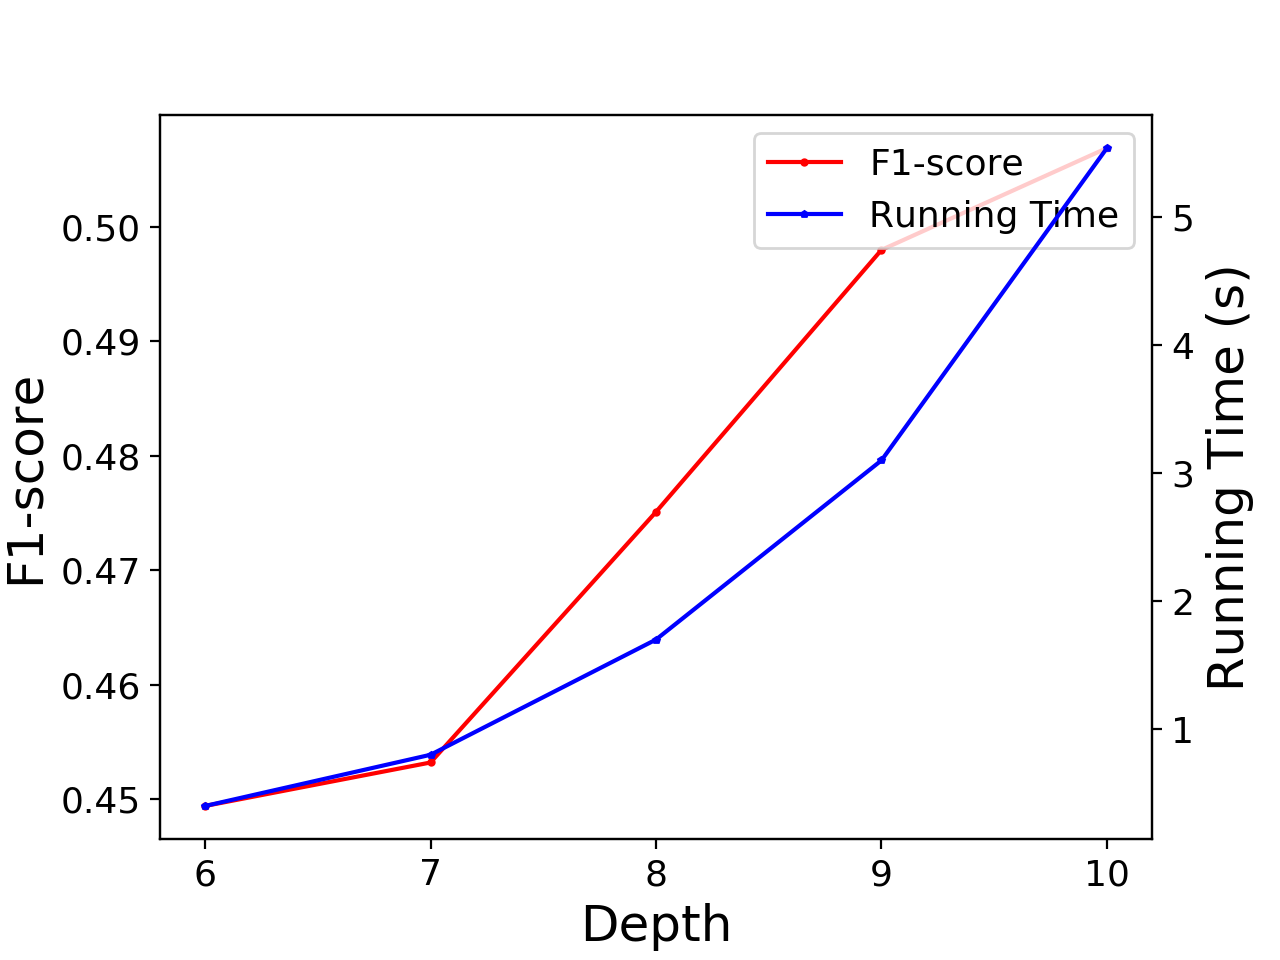
\includegraphics[width = 0.33\columnwidth]{img/chapter3/keyword.png}}
	\subfloat[Depth $d$  in Listening model]{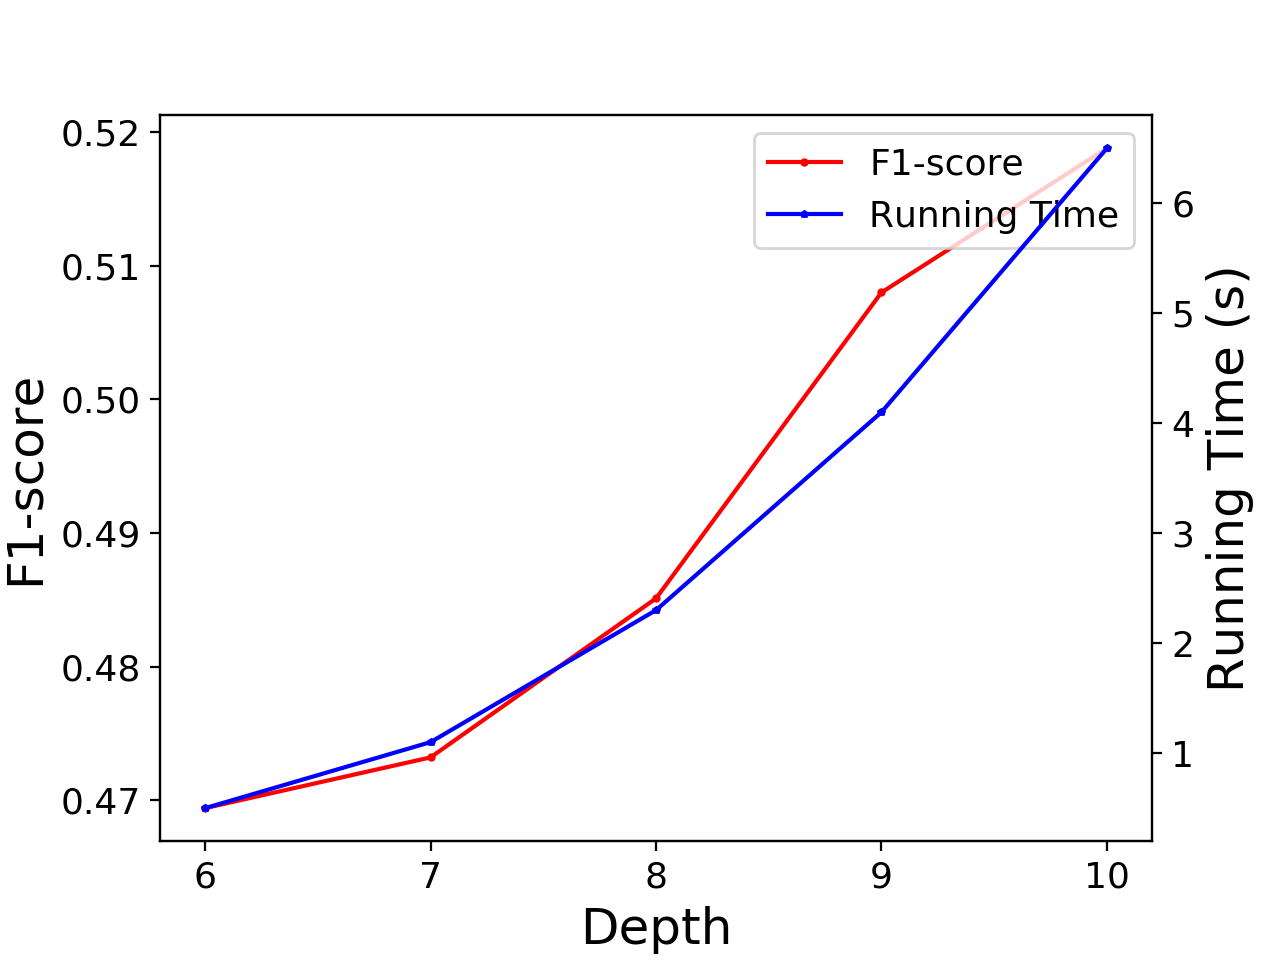
\includegraphics[width = 0.33\columnwidth]{img/chapter3/colisten.png}}  \\
	\subfloat[Iteration $T$ in all models]{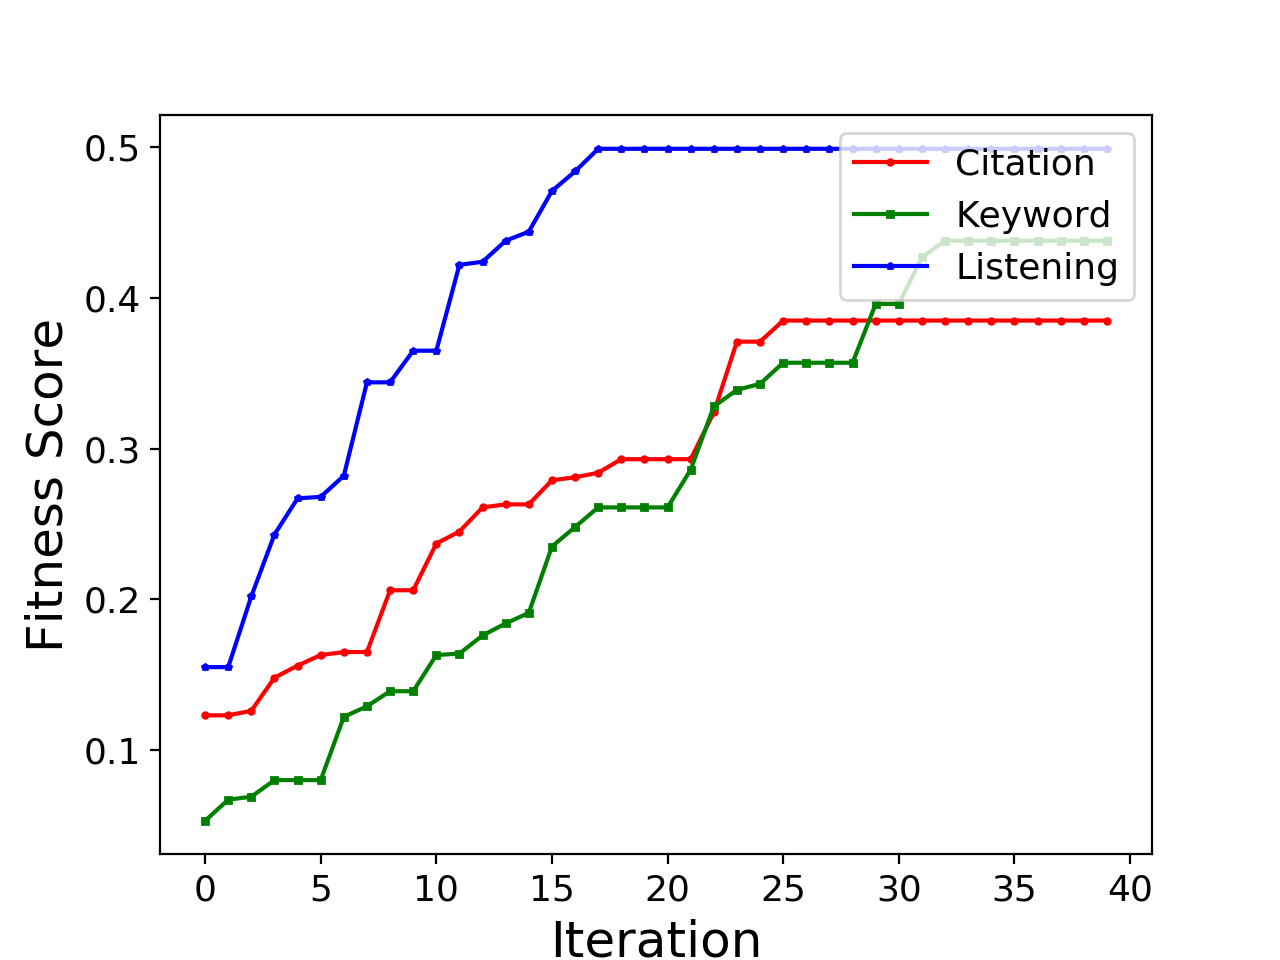
\includegraphics[width = 0.33\columnwidth]{img/chapter3/iteration.png}} 
	\subfloat[User searching preference $\lambda$ in all models]{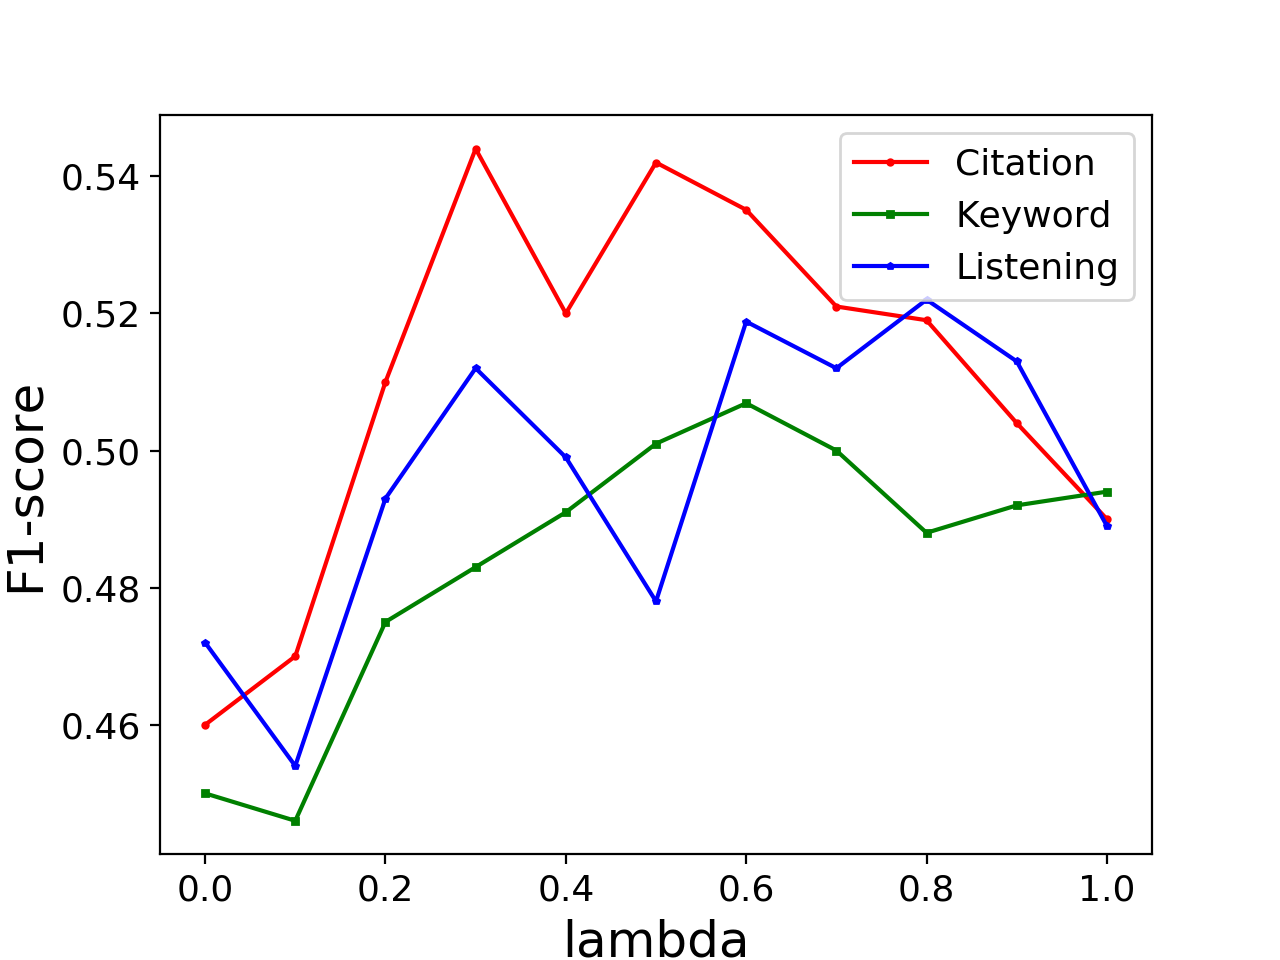
\includegraphics[width = 0.33\columnwidth]{img/chapter3/lambda.png}} 
	%	\vspace{-1em}
	\caption{Parameter effects on model performance}
	\label{fig:tuning}
	%	\vspace{-1em}
\end{figure}
I show how three parameters can affect my gPCD model performance in this section. They are the depth of the binary community tree $d$, genetic iteration number $T$ and user searching preference $\lambda$. Figure \ref{fig:tuning} show the overall impacts of all tuned parameters.



\textbf{Depth on the Tree}: Figure \ref{fig:tuning}(a) to  Figure \ref{fig:tuning}(c) show how the depth of the binary community tree affects the model performance in accuracy and efficiency. From the figures, larger depth leads to a better personalized community detection result, while causes an exponential running time increase at the same time. Based on empirical studies, the upper bound of the depth is set to be 10 in this paper. While the depth selection may varies based on different graph sizes.

\textbf{Convergence Analysis}: I observe the best chromosome updates in 40 iterations. From Figure \ref{fig:tuning}(d),   I can see the fitness score start to be stable after the 30 iterations, which means the best chromosome is no longer changed after around 30 iterations. Thus, I set $T = 30$ as the default iteration number in my approach.

\textbf{Searching Preference}: In Figure \ref{fig:tuning}(e), $\lambda$ reflects the user searching preference whether he/she wants to explore new information or avoid redundant information. By selecting $\lambda$ from 0 to 1, I find  the F1-score are not very stable or have a clear correlation with $\lambda$. Based on the empirical experiments, I achieve the best performance on three models when $\lambda = 0.6$.






%%%%%%%%%%%%%%%%
% Chapter 4
%%%%%%%%%%%%%%%%

%\chapter{Cross-Graph Community Detection}
\section{Introduction}

Community detection is an essential task for cyberspace mining, which has been successfully employed to explore users’ resemblance for retrieval/recommendation enhancement and user behavior analysis. Taking social media and e-commerce as examples, the complex, and often heterogeneous, relations among users and other objects, e.g., products, reviews, and messages, can be encapsulated as bipartite graphs, and the topology can help to synthesize and represent users with a coarser and broader view.

While a graph is well-connected, conventional methods, e.g., modularity-based approach \cite{newman2004fast}, spectral approach \cite{nascimento2011spectral}, dynamic approach \cite{peixoto2017modelling} and deep learning approach \cite{chiang2019cluster}, are able to estimate the internal/external connectivity and generate high-quality communities directly on nodes \cite{fortunato2016community}.
 
For sparse graphs, as mentioned in the Chapter \ref{ch:intro}, to deal with the lack-of-connection problem, I propose  a novel research task – Cross-Graph Community Detection. The idea is based on the fact that an increasing number of small apps are utilizing the user identity information inherited from giant providers, i.e., users can easily login a large number of new apps by using Facebook and Google ID. In such ecosystem, the main large graph can provide critical information to enlighten the community detection on many small sparse graphs. Note that, in spit of the small sparse graphs can engage with a specific field, the main graph is quite comprehensive and noisy. As Figure \ref{fig:c4_example} shows, not all the connections in Amazon (shopping graph) can be equally important for the two candidate app graphs. In the example, three mutual users are selected where $u_1$ and $u_2$ mainly share similar shopping interests on cosmetics and $u_1$ and $u_3$ mainly share similar shopping interests on food products in Amazon. Then, with deliberate propagation from main graph, in the Cosmetic graph, $u_1$ and $u_2$ have a better chance to be grouped together, while $u_1$ and $u_3$ are more likely to be assigned the same community ID in the Cooking graph. Therefore, the proposed model should be able to differentiate various kinds of information from the main graph for each candidate sparse graph to enhance its local community detection performance. 

As another challenge, small sparse graphs often suffer from training data insufficiency, e.g., the limited connections in these graphs can hardly tell the community residency information. In this study, I employed a novel data augmentation approach - cross-graph pairwise learning. Given a candidate user and an associated user triplet, the proposed model can detection the community closeness superiority by leveraging main graph and the sparse graph simultaneously. Moreover, the proposed pairwise learning method can cope with the main graph heterogeneity issue and reduce noisy information by taking care of graph local structure. Theoretically, I can offer at most $\mathcal{O}(N^{3})$ user triplets to learn graph community structure while conventional community detection methods by default can only be applied on $\mathcal{O}(N)$ users  ($N$ is the number of users in the sparse graph).

Therefore, I propose an innovative \textit{Pairwise Cross-graph Community Detection} (PCCD) model for enhanced sparse graph user community detection. Specifically, given user $u_i$ and its associated triplet $\langle u_{i},u_{j},u_{k}\rangle$, I aim to predict their pairwise community relationship, e.g., compared with user $u_{k}$, user $u_{j}$ should have closer, similar or farther community closeness to user $u_i$. 

\section{Method}
\begin{figure}  
	% \advance\leftskip-1cm 
	\centering
	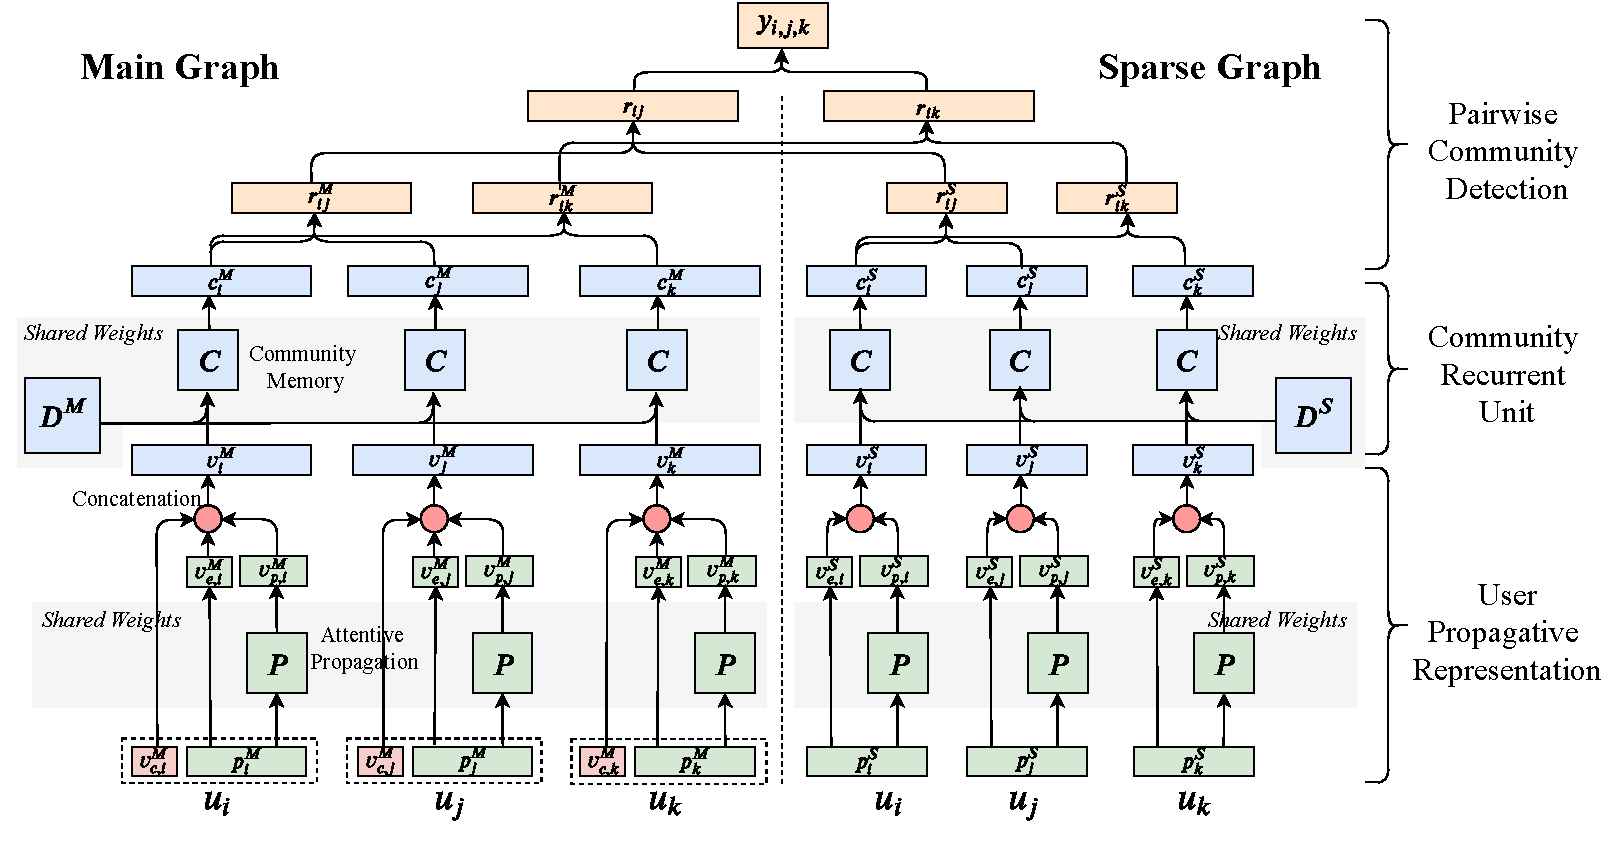
\includegraphics[width=1\columnwidth]{img/chapter4/pipeline.pdf}
	%  \vspace{-3em}
	\caption{The overall architecture of my proposed PCCD model. It contains three major modules mentioned in the right part of the figure. Each training instance is a mutual user triplet $\langle u_i,u_j,u_k \rangle$. Compared with the sparse graph, the main graph involves raw user community as part of model input.}
	
	\label{fig:c4_pipeline}
	%  \vspace{-1em} 
\end{figure}
\subsection{Task Overview} \label{sc:to}


As aforementioned, conventional methods suffer from graph sparseness problem. In this study, I propose a Pairwise Cross-graph Community Detection (PCCD) model that particularly aims at detecting user pairwise community closeness in sparse graphs by involving cross-graph techniques. 

Particularly, a well connected graph is called ``main graph" in this paper, corresponding to the targeted sparse graph. In general, as users may visit multiple cyber domains within a short time period, these mutual users co-occurred in both the main and sparse graph are taken as the bridge to connect the two graphs. Therefore, the relevant information from the main graph can be propagated to the sparse graph to support its user community detection. 

Specifically, my proposed model (showed in Figure \ref{fig:c4_pipeline}) is trained on mutual user triplets to learn three types of pairwise community relationship including ``\textit{similar}'', ``\textit{closer}'' and ``\textit{farther}''. The goal of this study can be reformulated as the following pairwise learning task: Given a sparse graph $S$ and a main graph $M$ where $N^C$ denotes their mutual user collection, for a mutual user triplet $\langle u_i,u_j,u_k \rangle  \in N^C$ (\textbf{Model Input}),  I aim to predict the relationship of its pairwise community closeness in graph $S$ (\textbf{Model Output}). In this paper, ``\textit{similar}'' relationship means that $u_j$ and $u_k$ are either in the same community or different communities with $u_i$. ``\textit{closer}'' relationship means that $u_j$ and $u_i$ are in the same community, while $u_k$ and $u_i$ are in different communities. ``\textit{farther}'' relationship means that $u_j$ and $u_i$ are in different communities, while $u_k$ and $u_i$ are in the same community.

For a mutual user triplet, my proposed model detects communities firstly on separate graphs to obtain all user raw community representations (Section \ref{sc:rcr}). Their propagative representations are learned through a community-level and a node-level filter (Section \ref{sc:upr}). Both representations are jointly utilized for predicting user community affiliation in each graph via a Community Recurrent Unit (Section \ref{sc:cru}). In the end, I integrate the community affiliation distributions to identify the pairwise community relationship of the triplet (Section \ref{sc:pcd}). Particular training strategies are introduced in the end (Section \ref{sc:mt}).

Note that even though my model is only trained on mutual users, it is still functional to detect pairwise community closeness on those users solely appeared in either the main or sparse graph. Further experiments in Section \ref{sc:ua} will verify its effectiveness on different types of users.

\subsection{Raw Community Representation} \label{sc:rcr}

As the user behavior is enriched in the main graph $M$, detecting user communities in it would offer auxiliary community features to potentially enhance my model performance. Therefore, I decide to involve user communities in the main graph as a part of model input. The same information from the sparse graph is intentionally omitted because its sparse graph structure is not able to offer reliable community partition results.

Considering all possible community detection methods listed in Section \ref{sc:baseline}, Infomap is empirically selected to detect user communities in the main graph $M$. Infomap method simulates a random walker wandering on the graph for $m$ steps and indexes his random walk path via a two-level codebook. Its final goal aims to generate a community partition with the minimum random walk description length, which is calculated as follows:

\begin{equation} 
\textit{$L(\pi)$} = \sum_{i}^{m}q_{\curvearrowright}^{i}H(\mathcal{Q})+\sum_{i=1}^{m} \textit{$p_{\circlearrowright}^{i}$}H(\textit{$\mathcal{P}^{i}$}) 
\end{equation}
where \textit{$L(\pi)$} is the description length for a random walker under current community partition $\pi$. $q_{\curvearrowright}^{i}$ and $p_{\circlearrowright}^{i}$ are the jumping rates between communities and within the $i_{th}$ community in each step. $H(\mathcal{Q})$ is the frequency-weighted average length of codewords in the global index codebook and $H(\mathcal{P}^{i})$ is frequency-weighted average length of codewords in the $i_{th}$ community codebook.


In the end, given a user $u_i$, I obtain its one-hot community representation $v_{c,i}^M$ in the main graph $M$, which is regarded as part of user representations for the model input.

\subsection{User Propagative Representation}\label{sc:upr}


\begin{figure}  
	% \advance\leftskip-1cm 
	\centering
	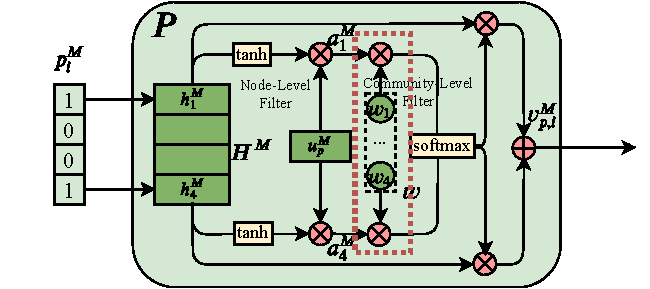
\includegraphics[width=\columnwidth]{img/chapter4/propagation.pdf}
	% 	\vspace{-1em}
	\caption{The two-level filter to support user propagative representation estimation in the main graph $M$. Sparse graph $S$ does not contain the community-level filter ( wrapped in the red rectangle).}
	\label{fig:propagation}
	% 	\vspace{-1.5em} 
\end{figure}

To better convey the mutual user insights in both main and sparse graph, their representations are learned from both direct transformation and weighted information propagation. The optimization processes are similar in the main and sparse graph. In the beginning, a user $u_i$ can be represented as a multi-hot embedding $p_{i}^{M}$ in the main graph $M$ (left part in Figure \ref{fig:propagation}) and $p_{i}^{S}$ in the sparse graph $S$. Each dimension in the embedding refers to a unique object with which the user connects in the related graph. 

The direct transformation from user multi-hot embedding learns a dense vector via one hidden layer so as to retrieve the compressed  information from user connected objects directly, which is calculated as follows:

\begin{equation}
v_{e,i}^{G} = {\rm tanh}(W_e^Gp_i^G + b_e^G) 
\end{equation}

where $G \in \{M, S\}$ denotes either the main or the sparse graph. $W_e^G$ and $b_e^G$ denote the weight matrix and bias respectively. $v_{e,i}^{G}$ is the learned direct transformation representation for user $u_i$.

On the other hand, from information propagation perspective, each object carries information, which can be propagated to its connected users as a type of representation. However, as such information are noisy and heterogeneous, not all of them are equally important to users. Therefore, a filtering module is proposed to automatically select appropriate information to propagate from both community level and node level.  The overall flow of the filtering module is illustrated in Figure \ref{fig:propagation}.

\textbf{Community-Level Filter:} As the raw detected communities in the sparse graph is not reliable because of graph sparseness, I only apply the community-level filter in the main graph $M$. According to the raw community partition $\pi$ calculated in Section \ref{sc:rcr}, each object node $n_i$ is assigned to a community $\pi(n_i)$. The community-level filter propagate object information in a coarser manner by considering its community importance weight $w_{\pi(n_i)}$. Throughout this filter, I aim to learn a weight vector $w$ where each dimension of $w$ denotes the importance score of a related community. 


\textbf{Node-Level Filter:} Node-level filter assesses the propagated information with a fine resolution. In the main graph $M$ ( a user-object bipartite graph), I aim to learn object representations $H^M = \{h_1^M,...,h_n^M\}$ where $h_n^M$ denotes the $n_{th}$ object representation. Similarly, $H^S$ denotes the object representations in the sparse graph $S$. The weight of the $j_{th}$ object node decides the amount of its information propagating to its connected user nodes, which is calculated in an attentive means: 

\begin{equation} \label{eq:np}
a_{j}^{G} = (u_p^{G})^{\intercal} {\rm tanh}(W^{G}_p h_{j}^{G} +b_p^{G})
\end{equation}

where $G \in\{M,S\}$ denotes either the main or the sparse graph. $u^{G}_p$ denotes the project vector in the related graph to calculate object attentive weights. $W_p^{G}$ and $b_p^{G}$ denote the corresponding weights and bias, respectively. 

I combine the community-level and node-level weights together to quantify the information propagation in the main graph $M$. While only the node-level weights is considered in the sparse graph $S$. Normalized by the ${\rm softmax}(\cdot)$ function, the related representation of  user $u_i$ in both graphs are calculated as follows:
\begin{equation}\label{eq:pv}
\begin{aligned} 
& v_{p,i}^{M} = \sum_{n_j \in \mathcal{N}^{M}(u_i)} {\rm softmax}(a_{j}^{M} w_{\pi(n_j)})  h_{j}^{M} \\
& v_{p,i}^{S} = \sum_{n_j \in \mathcal{N}^{S}(u_i)}{\rm softmax}(a_{j}^{S}) h_{j}^{S} 
\end{aligned} 
\end{equation}

Both $v_{p,i}^{M}$ and $v_{p,i}^{S}$ are the weighted sum of the neighbour object representations. $\mathcal{N}^{S}(n_i)$ and $\mathcal{N}^{M}(n_i)$ denote user connected objects in both graphs. 

Finally, given a user $u_i$, its raw community representation, direct transformation representation and two-level filtered representation construct its propagative representation in the main graph $M$. While its direct transformation representation and node-level filtered representation construct its propagative representation in the sparse graph $S$. To avoid gradient vanishing, a ${\rm batch\_norm(\cdot)}$ function is applied on top of the concatenated representations in both graph:
\begin{equation} \label{eq:nv}
\begin{aligned} 
& v_{i}^{M} = {\rm batch\_norm}([v_{c,i}^{M},v_{e,i}^{M},v_{p,i}^{M}]) \\
& v_{i}^{S} = {\rm batch\_norm}( [v_{e,i}^{S},v_{p,i}^{S}])
\end{aligned} 
\end{equation} 

\subsection{Community Recurrent Unit}\label{sc:cru}

After previous steps, each user of the mutual user triplet $\langle u_{i},u_{j},u_{k}\rangle$ is associated with a propagative representation. In this section, its corresponding community affiliation scores $c_{i}^{G}$ are further calculated in related graphs $G \in\{M,S\}$ through a designed Community Recurrent Unit (CRU), which is showed in Figure \ref{fig:cru}. The CRU contains an affiliation gate to calculate the user affiliation score for each community and an update gate to update community self representations. Within this unit, a community memory $D^{G} = \{d_1^G,...,d_K^G\}$ is designated to store $K$ community representations. Particularly, community representation is required to be with the same dimension as user propagative representation in both graphs.
\textbf{Community Affiliation Gate:} The affiliation gate helps to generate the affiliation score of a user $u_i$ towards each community in both graphs, which forms a $K$-dimensional vector $c_{i}^{G} = \{c_{i,1}^{G},...,c_{i,K}^{G}\}$ where $G \in \{M, S\}$ . The user $u_i$'s affiliation score $c_{i,j}^G$ towards the $j_{th}$ community in the graph $G$ is calculated as follows:

\begin{equation}\label{eq:dg}
c_{i,j}^G = {\rm  \sigma}((u_{c}^{G})^{\intercal}({\rm  tanh}(v_{i}^{G})*d_j^G))
\end{equation}

The dot product between transformed user propagative representation ${\rm  tanh}(v_{i}^{G})$ and the $j_{th}$ community representation $ d_j^G$ indicates their potential correlation, which further  turns to a scalar affiliation score $c_{i,j}^G$ between 0 to 1 with the help of a projection vector $u_{c}^{G}$ and normalization function $\sigma(\cdot)$.

\begin{figure}  
	% 	\advance\leftskip-2cm 
	\centering
	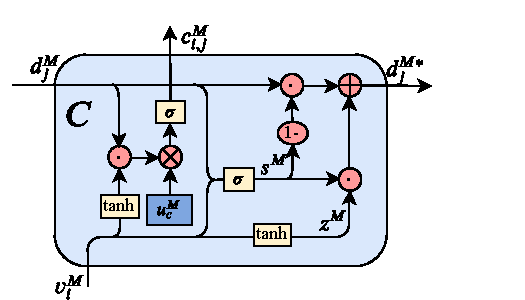
\includegraphics[width=1.2\columnwidth]{img/chapter4/cru.pdf}
	% 	\vspace{-1em}
	\caption{The flow of Community Recurrent Unit in the main graph $M$. The left part refers to the community affiliation gate and the right part is the community update gate.}
	\label{fig:cru}
	% 	\vspace{-1.5em} 
\end{figure}

\textbf{Community Update Gate: } \label{sc:cug} When calculating $u_i$'s community affiliation, its information can help to update community representations in return. The updated representation is relied on both previous step community representation and current user propagative representation. Therefore, to better embrace the two representations, I use a delicate RNN variant, where the update process is calculated as follows:

\begin{equation}\label{eq:up}
\begin{aligned}
&  s^G = \sigma(W_s^G[v_i^{G},d_j^{G}] + b_s^G) \\
& z^G = {\rm tanh}(W_z^Gv_i^G+b_z^G)\\
& d_j^{G*} = (1-s^G)*d_j^{G} + s^G*z^G
\end{aligned}
\end{equation}

where $G \in \{M,S\}$. $s^G$ denotes the update rate and $z^G$ is transformed user information to be updated in current community.  $d_j^{G*}$ denotes the updated representation of the $j_{th}$ community in graph $G$, which is the weighted sum on previous community and current user representations. $W_s^G$ and $W_z^G,$ denote related weight matrices, while $b_s^G$ and $b_z^G,$ denote related biases. 

\textbf{Community Constraint: }
To obtain the communities with less overlapping information in graph $G \in \{M,S\}$, the community representations ideally should be independent with each other. In my model, cosine similarity ${\rm cos}(\cdot)$ is taken as the criteria to measure the community similarity where higher score indicates stronger correlation. The averaged cosine similarities of all possible community representation pairs is calculated as a community loss to minimize:

\begin{equation}\label{eq:cc}
\mathcal{L}_{c}^{G} = \frac{1}{2K^2}\sum_{i,j}{\rm cos}(d_i^{G},d_j^{G})
\end{equation}
where $K$ is the number of communities in each graph.

\subsection{Pairwise Community Detection}\label{sc:pcd}

Similar to RankNet \cite{burges2010ranknet}, given a mutual user triplet  $\langle u_i,u_j,u_k \rangle$, as three types of pairwise label are considered including ``\textit{closer}'', ``\textit{similar}'' and ``\textit{farther}'', label $y_{i,j,k}$  is calculated as follows:
\begin{equation}\label{eq:y}
y_{i,j,k} = \frac{1}{2}(1+S_{jk})
\end{equation}
In terms of the community closeness for $u_i$, if $u_j$ is closer than $u_k$, $S_{jk} = 1$; if $u_j$ is farther than $u_k$, $S_{jk} = -1$; if $u_j$ and $u_k$ are similar, $S_{jk} = 0$. In this way, I convert the pairwise ranking task to a regression task. 

To optimize this task, first of all, I calculate the correlation representation $r^{G}_{ij}$ between $u_j$ and $u_i$ in single graph $G \in \{M,S\}$:

\begin{equation}\label{eq:gr}
r^{G}_{ij} = W^{G}_{r}(c_{i}^{G} - c_{j}^{G}) +  b^{G}_{r} 
\end{equation}

where $ W^{G}_{r}$ and $ b^{G}_{r}$ are related weight and bias, respectively. 

To construct the information from both graphs, I concatenate the correlation representations from both graphs:
\begin{equation} \label{eq:cr}
r_{ij} = {\rm tanh}([r^{S}_{ij},r^{M}_{ij}])
\end{equation}
Similarly, the cross-graph correlation representation  between $u_i$ and $u_k$ is calculated as $r_{ik}$. 

After that, I predict the community relationship between $u_j$ and $u_k$ towards $u_i$ as follows:
\begin{equation} \label{eq:yp}
\hat{y}_{i,j,k} = \sigma(W_{o}(r_{ij} - r_{ik}) +  b_{o})
\end{equation}

where $W_{o}$ and $b_{o}$ are the related weight and bias. $\sigma(\cdot)$ denotes the sigmoid activation function. In the end, the final loss $\mathcal{L}_{total}$ is the weighted sum of the optimization loss calculated via cross entropy and the community constraint losses where  $\mathcal{L}_{c}^S$ is for the sparse graph and $\mathcal{L}_{c}^M$ is for the main graph:
\begin{equation}\label{eq:loss}
\mathcal{L}_{total} = \underbrace{-y_{i,j,k}log\hat{y}_{i,j,k}-(1-y_{i,j,k})log(1-\hat{y}_{i,j,k})}_{optimization} + \underbrace{\alpha(\mathcal{L}_{c}^S + \mathcal{L}_{c}^M)}_{constraint}
\end{equation}

\subsection{Training Strategy}\label{sc:mt}

Although my model is trained solely on mutual user triplets, it is also able to detect pairwise community closeness among users only appeared in either sparse graph or main graph. Two training tricks are particularly employed in my model to improve model robustness, including shared weights and masked training. 

First, as my model should be insensitive to the sequence of input user triplet, the weight matrices, biases and project vectors in both Section \ref{sc:upr} and Section \ref{sc:cru} should be shared among the three users. Moreover, in  Section \ref{sc:cru}, the community memory $D^G$ where $G \in \{M,S\}$ is updated by taking the average of the three updated community representations (calculated in Eq. \ref{eq:up}) from input triplets.

Second, to alleviate the negative effects of excessive connections in main graph $M$, I employ a masked training strategy by randomly remove a small ratio $\rho$ of connected objects from users in the main graph during each training batch. $\rho = 0$ means users remain their original multi-hot embeddings while $\rho = 1$ means users lose all their connections on objects. 





\section{Experiments}  \label{sc:exp}
\subsection{Dataset}  \label{sc:dataset}
As one of the largest e-commerce ecosystems, Alibaba owns multiple online businesses, where users could try different services via the same login ID. For this experiment, I employ three services from Alibaba including an online shopping website, a digital news portal and a cooking recipe website. The online shopping website is regarded as the main graph because it is Alibaba core service having the largest number of active users. By contrast, the other two services are regarded as sparse graphs. In the online shopping website, each object refers to a product for sale, and links are user purchase behaviors on products. In the digital news portal, each object refers to a news article, and links are user reads on news. In the cooking recipe website, each object refers to a cooking recipe, and links mean that users follow recipe instructions. 

To prove my model robustness with respect to the graph size, two cross-graph datasets are constructed in different scales, which are showed in Table \ref{tab:dataset}. The SH-NE dataset is the cross-graph dataset constructed by the shopping graph and news graph, which is ten times larger than the SH-CO dataset constructed by the shopping graph and recipe graph. Users are categorized into three different types including \textit{MU} (mutual users appeared in both graphs),  \textit{MO} (users only appeared in the main graph), and  \textit{SO} (users only appeared in the sparse graph). Note that, only mutual user triplets are used for training.

\begin{table}[h]
	% \scriptsize
	
%	\small
	\centering
%	\renewcommand{\tabcolsep}{1.5pt}
	% \renewcommand\arraystretch{0.5}
	\begin{tabular}{|c|c|c|c|c|c|c|c|c|} 
		\hline
		\multirow{2}{*}{\textbf{Dataset}}& \multirow{2}{*}{\textbf{\#MU}}&\multicolumn{3}{c|}{\textbf{Main Graph}}& \multicolumn{3}{c|}{\textbf{Sparse Graph}}\\ \cline{3-8}
		&  &\textbf{\#MO}&\textbf{\#Object}& \textbf{\#Link}&\textbf{\#SO}&\textbf{\#Object}& \textbf{\#Link}\\ \hline
		\textbf{SH-NE}& 105,702 & 392,549 & 135,320 & 17,352,482  & 26,133 & 9,377 & 881,721\\ 
		\textbf{SH-CO}& 1,029  & 1,543  &23,881 & 1,161,293& 719  & 3,739 &147,266\\\hline
	\end{tabular}
	% 	\vspace{-0.5em} 
	\caption{Statistics of Two cross-graph datasets.}
	\label{tab:dataset}
	% 	\vspace{-1em} 
\end{table}  

Both datasets are built by taking a week of user behaviors from 09/20/2018 to 09/26/2018. In this paper, for two sparse graphs, I aim to predict user pairwise community labels (calculated from enriched seven-day user behaviors) using sparse user behaviors (the first four-day user behaviors, arbitrarily defined in this paper).

To construct my ground truth data, I run all baseline models (will be introduced in Section \ref{sc:baseline}) on both seven-day sparse graphs which are assumed to contain sufficient information for detecting user communities. Only mutual user communities agreed by all seven baselines are kept, from which mutual user triplets are subsequently selected. In this paper, I define three types to label pairwise community closeness for a mutual user triplet, including ``\textit{closer}'', ``\textit{similar}'', and ``\textit{farther}'' (detailed definition is in Section \ref{sc:to}). Equal number of triplets are randomly selected for each label type. In total, there are 207,291 triplets in SH-NE dataset and 20,313 triplets in SH-CO dataset for testing propose. 

Training data generation is the same as ground truth data construction except using first four-day user behaviors. In total, there are 2,072,905 triplets in SH-NE dataset and  203,123 triplets in SH-CO dataset, from which 90\% of the triplets are used for training and 10\% for validation.

In both training and testing process, my model input is user triplets with first four-day behavior information. Their difference is that the pseudo labels for training are generated from four-day user behaviors, while the ground truth labels for testing are generated from whole seven-day user behaviors in sparse graphs.


\subsection{Baselines and Settings} \label{sc:baseline}
As there is neither reliable nor open-sourced studies on pairwise cross-graph community detection, I have no direct comparative models. In this paper, I select one random model and six compromised but state-of-art baselines which are originally designed for whole graph community detection. In the first seven baselines, after user communities are detected, I calculate user triplet labels via Eq. \ref{eq:y}. As all baselines are trained on the sparse graph with first four-day user behavior and the main graph, they bring no information loss compared with my model. Here is the details of how these baselines calculate user communities:

\begin{itemize}
	\item \textbf{random}: users are randomly assigned to a given number of communities.
	\item \textbf{Infomap} \cite{rosvall2011multilevel}: A random walk based method to detect user communities by minimizing description length of walk paths.\footnote{https://github.com/mapequation/infomap}
	\item \textbf{DNR} \cite{yang2016modularity}: A novel nonlinear reconstruction method to detect communities by adopting deep neural networks on pairwise constraints among graph nodes.\footnote{http://yangliang.github.io/code/}
	\item \textbf{LSH} \cite{chamberlain2018real}: A random walk based method for community detection in large-scale graphs.\footnote{https://github.com/melifluos/LSH-community-detection}
	\item \textbf{Node2vec} \cite{grover2016node2vec}: A skip-gram model to generate node emebeddings based on guided random walks on graphs. And K-means method subsequently calculates communities from the generated embeddings.\footnote{https://github.com/snap-stanford/snap/\label{fn:snap}}
	\item \textbf{BigClam} \cite{yang2013overlapping}: A non-negative matrix factorization method to detect overlapping communities in large scale graphs.\footref{fn:snap}
	\item \textbf{WMW} \cite{castrillo2017fast}: A fast heuristic method for hierarchical community detection inspired by agglomerative hierarchical clustering.\footnote{https://github.com/eduarc/WMW} 
\end{itemize}

The result is reported with best hyper-parameters from grid search. Empirically, a mini-batch (size = 200) Adam optimizer is chosen to train my model with learning rate as 0.01. Community number on both graphs is $K = 50$ (Eq. \ref{eq:cc}). Community constraint weight is $\alpha = 0.1$ (Eq. \ref{eq:loss}). Masked training rate in the main graph is $\rho = 0.05$. The model is trained for 1000 epochs in order to get a converged result. 

Model performance is evaluated from both classification and retrieval viewpoints. From classification aspect, Accuracy (ACC), F1-macro (F1) and Matthews Correlation Coefficient (MCC) are reported metrics.
From retrieval aspect, Mean Reciprocal Rank (MRR), Normalized Discounted Cumulative Gain (NDCG) and Mean Average Precision (MAP) are reported metrics. All of them are fundamental metrics widely used for model evaluation.  
\section{Discussion}
\subsection{Performance Comparison}
\begin{sidewaystable}[h]
	%	\scriptsize
	
	% 	\small
	\centering
	\renewcommand{\tabcolsep}{2.5pt}
	%	\renewcommand\arraystretch{0.5}
	\begin{tabular}{cccccccccccccc} 
		\toprule
		\multirow{2}{*}{ \textbf{Graph}} & 	\multirow{2}{*}{\textbf{Model}}	&\multicolumn{6}{c}{\textbf{SH-NE Dataset}} & \multicolumn{6}{c}{\textbf{SH-CO Dataset}}\\
		\cmidrule(lr){3-14}
		& & \textbf{ACC}& \textbf{F1}& \textbf{MCC}& \textbf{MRR}& \textbf{NDCG}& \textbf{MAP} & \textbf{ACC}& \textbf{F1}& \textbf{MCC} & \textbf{MRR}& \textbf{NDCG}& \textbf{MAP} \\ \midrule 
		\multirow{6}{*}{\textbf{Main }} &random  & 0.3324& 0.1677&-0.0001&0.7719&0.8373&0.7299&0.3302&0.1700&0.0027&0.7842&0.8444&0.7401\\ 
		& Infomap &0.3700& 0.2731&0.1201&0.8334&0.8421&0.7299 &0.3811&0.3723&0.1000&0.7888&0.8419&0.7430\\  
		& DNR &0.4210&0.4022&0.1789&0.8000&0.8366&0.7473&0.5194&0.5122&0.2712&0.8099&0.8773&0.7592\\   
		& LSH &0.3798&0.3813&0.0888&0.8002&0.8433&0.7328&0.4000&0.4123&0.1277&0.7812&0.8329&0.7570\\ 
		& node2vec& 0.4888 &0.5014&0.2521&0.8229&0.8744&0.7832&0.5959&0.5832&0.3895&0.8422&0.8936&0.8222\\   
		& BigClam &0.5555&0.5399&0.3349&0.8421&0.8890&0.8024&0.5301&0.5334&0.3290&0.8335&0.8573&0.8005\\ 
		& WMW &0.6032&0.6158&0.4111&0.8632&0.8988&0.8256&0.6489&0.6661&0.5001&0.8789&0.9032&0.8499\\ \midrule 
		\multirow{6}{*}{\textbf{Sparse}} &random  & 0.3333& 0.1785&0.0003&0.7815&0.8438&0.7419&0.3301&0.1720&0.0030&0.7801&0.8400&0.7338\\ 
		& Infomap &0.3455& 0.1929&0.0031&0.7843&0.8399&0.7437 &0.3676&0.3211&0.0422&0.7905&0.8446&0.7401\\  
		& DNR &0.4433&0.4407&0.2020&0.8313&0.8678&0.7742&0.5273&0.5289&0.2787&0.8293&0.8765&0.7980\\   
		& LSH &0.3889&0.3917&0.0942&0.8008&0.8528&0.7343&0.4093&0.4177&0.1138&0.7833&0.8438&0.7404\\ 
		& node2vec& 0.4849 &0.4958&0.2467&0.8219&0.8664&0.7774&0.5732&0.5746&0.3898&0.8412&0.8823&0.8146\\   
		& BigClam &0.5277&0.5355&0.3332&0.8441&0.8750&0.8005&0.5282&0.5280&0.3339&0.8298&0.8399&0.8033\\ 
		& WMW &0.5814&0.5900&0.3988&0.8666&0.9001&0.8210&0.5911&0.6212&0.4347&0.8599&0.8890&0.8133
		\\ \midrule 
		\multirow{7}{*}{\textbf{\makecell{Main \\ + \\ Sparse}}} &random  & 0.3337& 0.1788&-0.0008&0.7815&0.8387&0.7387&0.3291&0.1699&0.0027&0.7739&0.8331&0.7310\\ 
		& Infomap &0.3625& 0.2567&0.0908&0.7864&0.8423&0.7437 &0.3930&0.3988&0.0916&0.7951&0.8488&0.7528\\  
		& DNR &0.4383&0.4204&0.1817&0.8101&0.8599&0.7686&0.5273&0.5322&0.2957&0.8391&0.8812&0.8000\\   
		& LSH &0.3992&0.4052&0.0993&0.8020&0.8538&0.7599&0.4180&0.4237&0.1309&0.8021&0.8539&0.7600\\ 
		& node2vec& 0.5072  &0.5124&0.2611&0.8339&0.8774&0.7943&0.6015&0.6055&0.4045&0.8677&0.9023&0.8324\\   
		& BigClam &0.5580&0.5626&0.3412&0.8511&0.8901&0.8135&0.5398&0.5383&0.3389&0.8475&0.8874&0.8095\\ 
		& WMW &0.6168&0.6205&0.4281&0.8702&0.9042&0.8353&0.6682&0.6711&0.5041&0.8879&0.9173&0.8561\\ 
		% 		iterative& 0.5587 & 0.5605  &  0.3593&0.6761&0.6788&0.5174 \\   
		& \textbf{PCCD}& \textbf{ 0.6524*}& \textbf{0.6551*} &  \textbf{0.4808*}& \textbf{0.8802*} & \textbf{0.9116*} & \textbf{0.8470*}& \textbf{0.7740*}& \textbf{0.7758*} &  \textbf{0.6627*}& \textbf{0.9244*} & \textbf{0.9442*} &  \textbf{0.9005*}
		\\ \bottomrule
	\end{tabular}
	% 	\vspace{-0.5em} 
	\caption{All model performances for three different graph combinations in two datasets. Symbol `*' highlights the cases where our model significantly beats the best baseline with $p<0.01$.}
	\label{tab:c4_evaluation}
	% 	\vspace{-1em} 
\end{sidewaystable}

All model performance are evaluated from both classification and retrieval viewpoints. Each baseline method is run on three graphs including the main graph, the sparse graph, and their combined graph. While our model can only be tested by utilizing both graphs. Table \ref{tab:c4_evaluation} shows the overall model performance under three graphs. Particularly, we run our model ten times and report the average performance result. To verify our model's superiority, we calculate the performance differences between our model and the best baseline on each metric for all the runs, and apply a pairwise t-test to check whether the performance difference is significant.

Our model output is a predicted score in the range from 0 to 1. Its associated label is assigned to be one of ``\textit{closer}'', ``\textit{similar}'' or ``\textit{farther}'' based on which third the predicted score lies in (associated with label definition in Section \ref{sc:pcd}). For example, a user triplet $\langle u_i,u_j,u_k \rangle$ with score 0.3 will be labelled as ``\textit{farther}'', which means compared with $u_k$, $u_j$ is has a farther community closeness to $u_i$. After that, from classification perspective, ACC, F1 and MCC scores are calculated by comparing predicted labels with the ground truth labels. While from retrieval perspective, MRR, NDCG and MAP are calculated for the pairwise ranking within user triplets.

Table \ref{tab:c4_evaluation} shows that all baseline performances in the combined graph achieve the best among three types of graphs. And performances in the main graph are always better than in the sparse graph. It demonstrates that main graph holds beneficial information to reveal user potential communities in sparse graphs. The random baseline is with similar performance among all three graphs, which makes sense because the random community partition is regardless of graph structures. It can be used as the default model to compare with in each graph. For the rest six baselines, random walk based baselines (Infomap and LSH) do not perform well in all three graphs. Their evaluation results are just a bit better than random model performance. WMW model performs the best among all baselines. Actually, its results are always the best in three graphs of both datasets. However, by taking the pairwise t-test, it statistically proves that our model still significantly outperforms the WMW model in terms of all metrics.

It is also interesting to see that the model evaluation results are consistent in all datasets. For example, DNR model always performs better than LSH model. The only exception is that BigClam performs better than node2vec in SH-NE dataset, but worse in SH-CO dataset. 

\subsection{Ablation Study}
\begin{table}[h]
	%	\scriptsize
	
	% 	\small
	\centering
%	\renewcommand{\tabcolsep}{3pt}
	%	\renewcommand\arraystretch{0.5}
	\begin{tabular}{cccccccc} 
		\toprule
		\textbf{Dataset}& \textbf{Model}	
		& \textbf{ACC}& \textbf{F1}& \textbf{MCC}& \textbf{MRR} & \textbf{NDCG}& \textbf{MAP}\\ \midrule 
		\multirow{5}{*}{ \textbf{SH-NE}} & -- RCR  &-2.61&-2.51&-3.76&-0.73&-0.54&-0.96\\
		& -- DTR &-1.32&-1.49&-2.96&-1.01&-0.14&-0.57\\ 
		& -- NF &-17.31&-17.01	&-25.92&-5.35&-3.88&-6.05\\
		& -- CF &-7.94&-8.48&-11.71&-2.61&-1.92&-3.01\\
		& -- CC &-2.15&-2.05&-3.08&-0.49&-0.35&-0.65\\ 
		& -- MT &-2.43&-2.55&-4.82&-0.78&-0.82&-1.24\\ 
		\midrule 
		\multirow{5}{*}{ \textbf{SH-CO}} & -- RCR &-2.13&-2.45&-3.07&-1.65&-0.58&-0.79  \\  
		& -- DTR &-3.45&-2.89&-1.95&-2.22&-0.43&-0.88\\ 
		& -- NF &-26.13&-25.83&-39.97&-9.81&-7.50&-19.35\\ 
		& -- CF &-21.12&-5.53&-8.45&-2.03&-1.50&-2.50\\
		& -- CC &-4.32&-4.34&-6.57&-1.56&-1.24&-1.91\\
		& -- MT &-1.32&-1.24&-2.66&-0.33&-0.21&-0.45\\ \bottomrule
	\end{tabular}
	% 	\vspace{-0.5em} 
	\caption{Performance differences on all evaluation metrics between each ablated model and the original model. ``-'' refers to remove related component from our model. Results are scaled in percentage (\%).}
	\label{tab:c4_ablation}
	% 	\vspace{-1em} 
\end{table} 
In this section, we aim to explore whether all components of our proposed model have positive effect on final model performance and which component has the largest impact. There are six components that can be disassembled from the main model, including Raw Community Representation in the main graph (RCR), Direct Transformation Representation (DTR), Node-level filter (NF), Community-level filter (CF), Community Constraint (CC) and Masked Training (MT). We iteratively remove each component while keep the rest firmed to demonstrate their performance difference compared to the original model. All comparison results are showed in Table \ref{tab:c4_ablation}.


Among the six components, if we remove node-level filter, the performance drop dramatically, even worse than some of baseline models. It indicates that node-level information are excessive and noisy. Without appropriate filtering on the propagated information, it would vitally pollute the quality of user representations. Similarly,  community-level filter also has a huge impact on model performance, meaning filtering propagated information from a coarser view also has a positive effect on learning user representations. By contrast, the two extra representations (RCR and DTR) do not have strong influence in our model. Having these information can slightly improve model performance as they still involve extra information. However, as one-hot embeddings, the amount of new information that RCR can offer is very limited. Similarly, DTR is only one-layer transformation on multi-hot embeddings. The information it can offer is also limited. By adding extra constraint, CC also has a little positive effect to enhance model performance. But as we always set its weight with a small value in training process, its influence is also indifferent. MT has the least impact on model performance as randomly masking user behaviors in the main graph has an overlapped effect with attentive weights calculated from the node-level filter in Section \ref{sc:upr}.

\subsection{User-Type Analysis}
\label{sc:ua}
\begin{table}[h]
	%	\scriptsize
	
	% 	\small
	\centering
%	\renewcommand{\tabcolsep}{3.5pt}
	%	\renewcommand\arraystretch{0.5}
	\begin{tabular}{cccccccc} 
		\toprule
		\textbf{Dataset}& \textbf{User}	
		& \textbf{ACC}& \textbf{F1}& \textbf{MCC}& \textbf{MRR} & \textbf{NDCG}& \textbf{MAP}\\ \midrule 
		\multirow{3}{*}{ \textbf{SH-NE}} & MU & 0.7132 & 0.7133 & 0.6012&  0.9112 & 0.9324 & 0.8704  \\   
		& MO & 0.6356 & 0.6477 & 0.4780&  0.8739 & 0.9002 & 0.8418 \\
		& SO & 0.6009 & 0.6117 & 0.4324&  0.8600 & 0.8988 & 0.8393 \\
		\midrule 
		\multirow{3}{*}{ \textbf{SH-CO}} & MU & 0.7852& 0.7780& 0.6724& 0.9300& 0.9474& 0.9015 \\   
		& MO & 0.7334& 0.7565& 0.6601& 0.9012& 0.9400& 0.8874\\
		& SO & 0.6823& 0.6915& 0.6844& 0.8990& 0.9222& 0.8789 \\ \bottomrule
	\end{tabular}
	% 	\vspace{-0.5em} 
	\caption{Three types of user performance in two datasets.}
	\label{tab:ua}
	% 	\vspace{-1em} 
\end{table} 

As aforementioned in Section \ref{sc:dataset}, there are three types of users in our cross-graph datasets including \textit{MU} (mutual users appeared in both graphs),  \textit{MO} (users only appeared in the main graph), and  \textit{SO} (users only appeared in the sparse graph). Unlike our training data which is constructed only with mutual users, our testing data can be with all types of users. To examine our model performance on each type of users, user triplets with only single type of users are screened, i.e., an eligible user triplet only contains three \textit{MO} type users. In fact, the performance on \textit{MO} user triplets reflects the capability of our model to solve cold-start problem as these users have no behaviors in the sparse graphs. The result showed in Table \ref{tab:ua} demonstrates that the label of \textit{MU} triplets can be best identified, which makes sense as the information of mutual users come from both graphs. While performance results on \textit{MO} are better than \textit{SO} user triplets, which might because that users are likely to have more enriched behaviors in the main graph compared with the sparse graph. Even that, the performance of our model on \textit{SO} user triplets is still better than most of baselines running on the combined graph.

\subsection{Graph Sparsity Influence}
\begin{figure}
	%\hspace*{-1cm} 
	\centering
	%%\subfloat[BLEU]{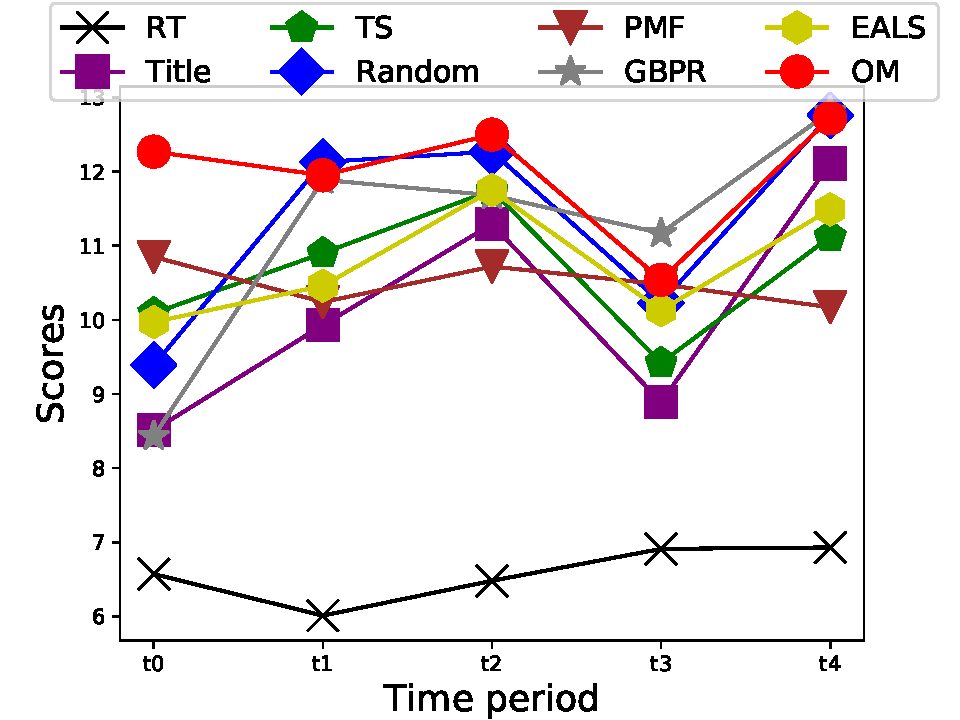
\includegraphics[width = 1.5in]{img/bleu.pdf}}  
	\subfloat[ACC]{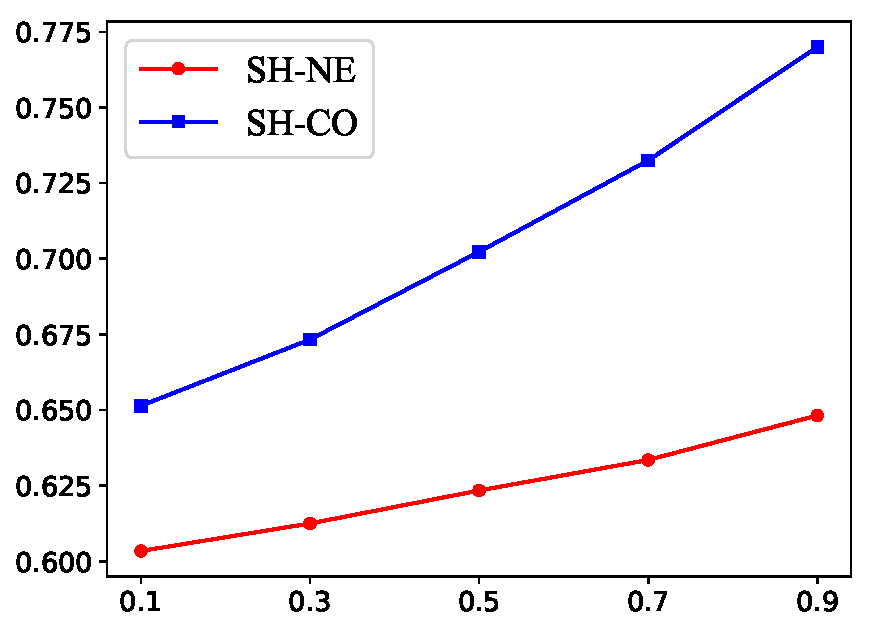
\includegraphics[width = 2in]{img/chapter4/acc.pdf}} 
	\subfloat[F1]{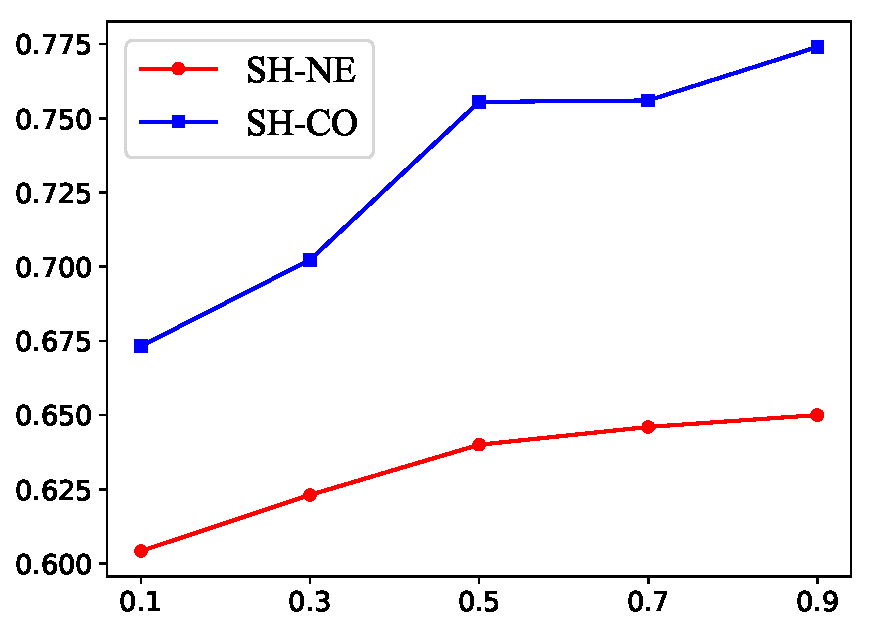
\includegraphics[width = 2in]{img/chapter4/f1.pdf}} 
	\subfloat[MCC]{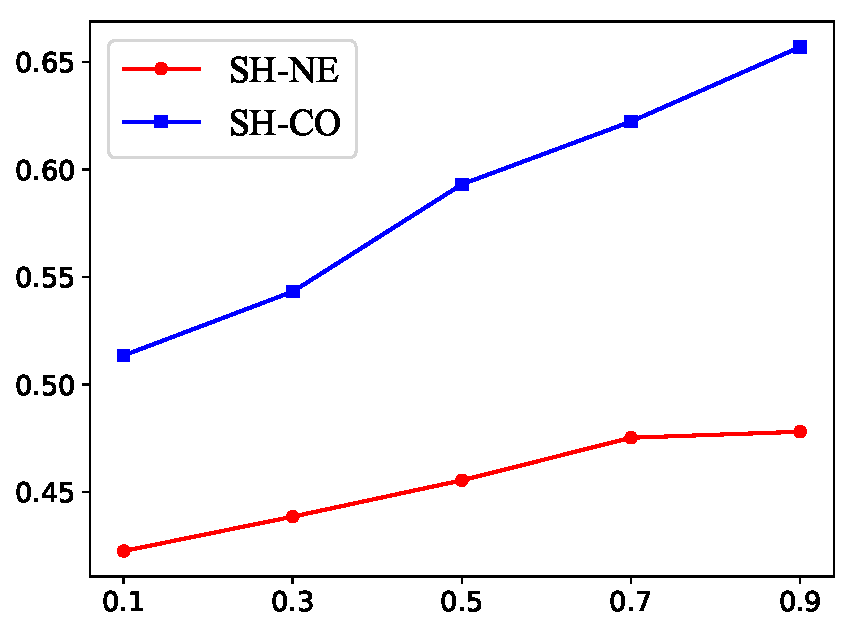
\includegraphics[width = 2in]{img/chapter4/mcc.pdf}}\\ 
	\subfloat[MRR]{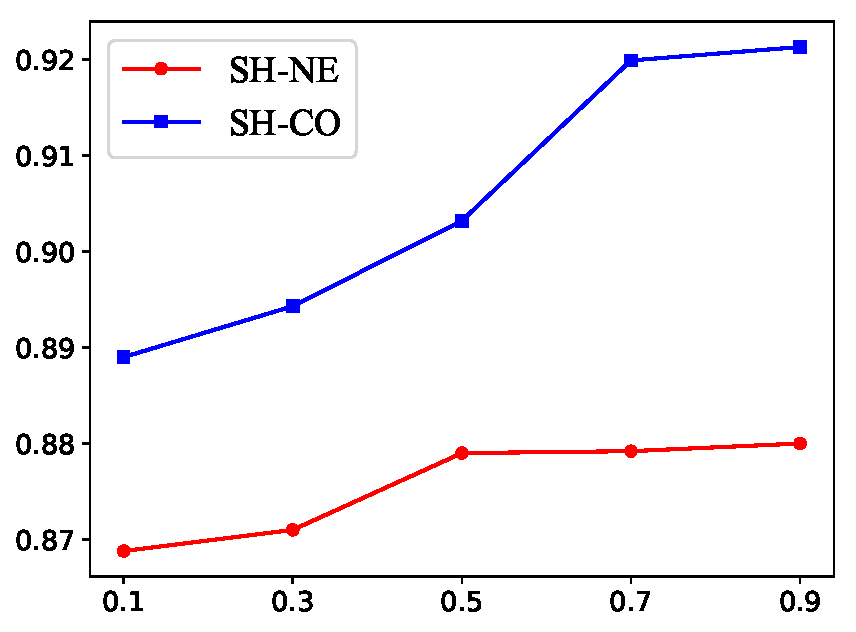
\includegraphics[width = 2in]{img/chapter4/mrr.pdf}} 
	\subfloat[NDCG]{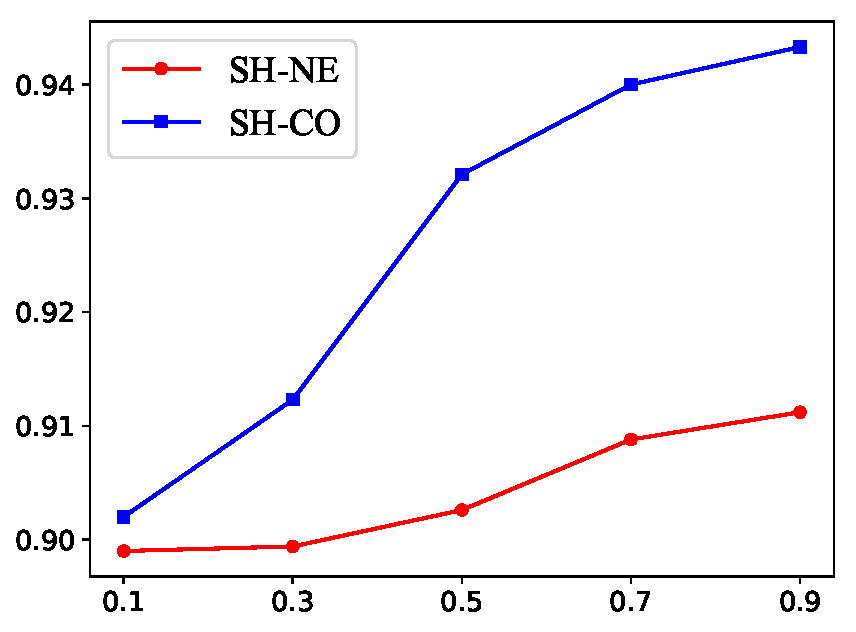
\includegraphics[width = 2in]{img/chapter4/ndcg.pdf}} 
	\subfloat[MAP]{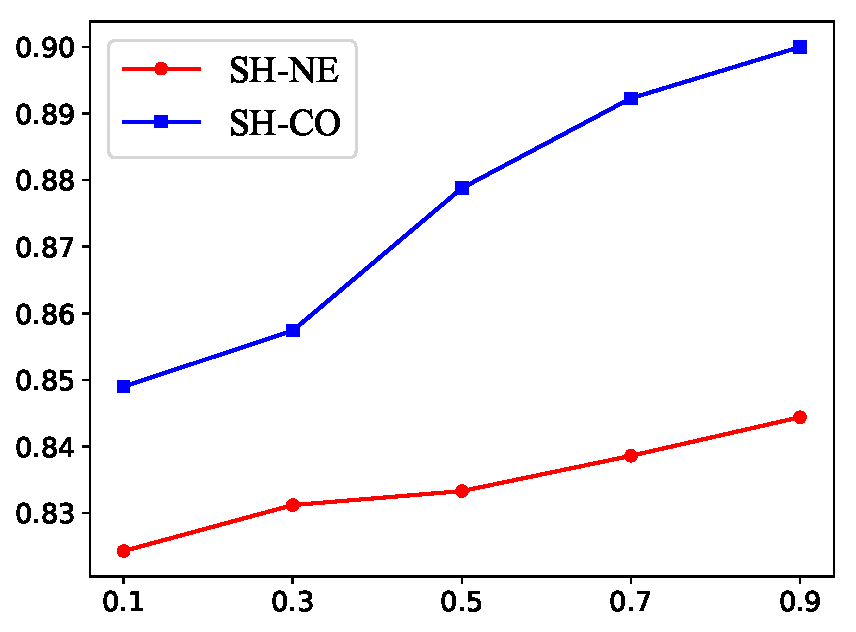
\includegraphics[width = 2in]{img/chapter4/map.pdf}} 
	\caption{Our model performance on all metrics under different graph sparsity scales. X-axis is the ratio of links preserved in the sparse graph. Y-axis is related metric score.}
	% 	 \vspace{-1em}
	\label{fig:sparsenss}
	% 	\vspace{-1em} 
\end{figure}
To explore our model robustness on graph sparsity, we randomly keep $\delta$ ratio of the total links in the sparse graph, where  $\delta=\{0.1,0.3,0.5,0.7,0.9\}$. Our model is trained on the whole main graph and each truncated sparse graph. The reported evaluation metrics under all sparse graphs with varied scales are visualized in Figure \ref{fig:sparsenss}. All metrics in both SH-NE and SH-CO datasets are in a rising trend with more links preserved in related sparse graphs. Compared with SH-NE dataset, SH-CO can benefit more from the sparse graph as it has a larger increase in all reported metrics. 

With more links are preserved, all evaluation metrics first grows rapidly. While the increasing speed slows down when 70\%-90\% links are preserved. This phenomenon can be seen in almost all plots in Figure \ref{fig:sparsenss}. It can be explained by the law of diminishing marginal utility, meaning that the marginal utility to bring new information derived from each additional link is declined.

Although classification related  metrics significantly increase with more links preserved (i.e., F1 score in SH-CO dataset increases 10\% when involving sparse graph), the retrieval related metrics (MRR, NDCG and MAP) do not change much in the mean time. One possible reason is that the information from the main shopping graph already contains enough information for the pairwise ranking in user triplets. For example, without considering sparse graph information, our model has already achieved high MRR score as 0.87 in SH-NE dataset and 0.89 in SH-CO dataset, which is already better than most baseline results running on the combined graph.


\subsection{Case Study}
In order to testify whether our proposed Community Recurrent Unit is able to accurately calculate user affiliation scores in each community, we choose three users (labelled from user $u_1$ to user $u_3$) and calculate their affiliation scores of ten selected communities (labelled from community $c_1$ to community $c_{10}$) in the main shopping graph. The detailed result is visualized in Figure \ref{fig:case}. In the left part of the figure, darker color indicates higher affiliation scores in the range from 0 to 1. Besides, in the shopping graph, we also extract all products purchased by each user, and manually select the most representative ones summarized as keywords in a table, which is demonstrated in the right part of Figure \ref{fig:case}.

From the right-part table, $u_1$ and $u_2$ share similar shopping interests in clothing products. $u_2$ is more like a girl fond of sports. And $u_1$ more tends to be a fashion girl. While the shopping interests of $u_3$ is much far away from the other users. All purchased products by $u_3$ is furnishing stuffs. It seems s/he is decorating her/his living space. Referring to the left part of Figure \ref{fig:case}, the affiliation distribution among ten communities between $u_1$ and $u_2$ are very similar. They both have a high weight in community $c_1$, $c_7$ and $c_8$. While the community distribution of $u_3$ is totally different. $u_3$ is heavily affiliated with community $c_2$. The results of our calculated community affiliation distribution is consistent with actual user behaviors, which indicates our Community Recurrent Unit (CRU) is  functional well to reflect user community information.
\begin{figure}  
	% \advance\leftskip-1cm 
	\centering
	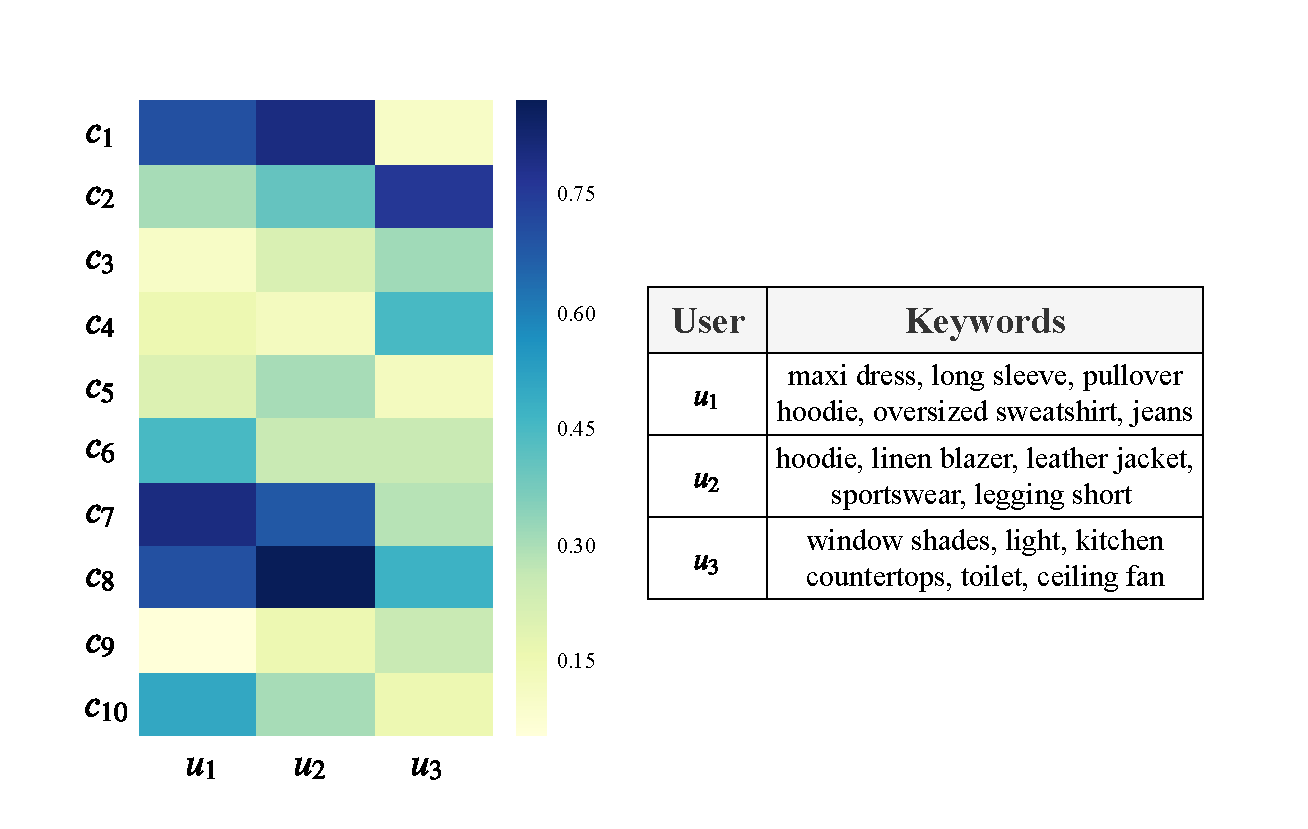
\includegraphics[width=1\columnwidth]{img/chapter4/case.pdf}
	%  \vspace{-3em}
	\caption{The left part shows ten community affiliation scores of three selected users in the shopping graph. The right part shows the keywords of their purchased products.}
	
	\label{fig:case}
	%  \vspace{-1em} 
\end{figure}





%%%%%%%%%%%%%%%%
% Chapter 5
%%%%%%%%%%%%%%%%

\chapter{Semi-Supervised Explainable Community Detection in Dynamic Graphs}
\section{Introduction}

Understanding product aspect-sentiments and tracking its changes in a timely manner can support better decision-making for commercial purposes, such as enlightening online retailers to make timely sales plans. Therefore, the \textit{Dynamic Summarization on Product Aspects} task is of great importance. It not only indicates products' dynamic aspect-sentiment changes, but also depicts the changes into readable contexts for easier interpretation.

Prior investigations on another similar topic, review summarization, mainly follow Natural Language Generation (NLG) approaches, such as using new Recurrent Neural Network (RNN) variant that uses gated connections to construct a character-level text generation mode or designing a multi-task model to predict rating and generate review summarization simultaneously using pairwise user-product relationship. Memory network is also used for review summarization generation. 
\begin{figure}  
	% \advance\leftskip-1cm 
	\centering
	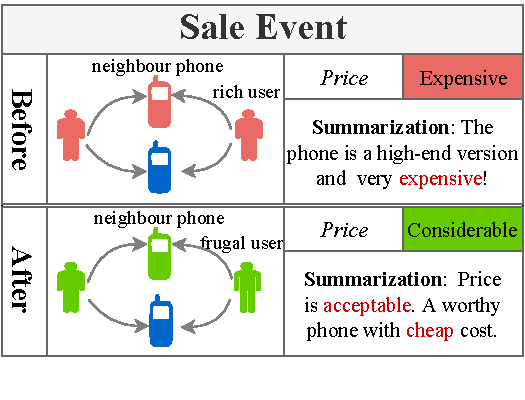
\includegraphics[width=0.8\columnwidth]{img/chapter5/example.pdf}
	% 	\vspace{-1em}
	\caption{An example to illustrate how to dynamically select neighbour products (red phone $\rightarrow$ green phone) for depicting current product (blue phone) sentiment change before \& after a sale event from user behaviors.}
	\label{fig:c5_example}
	% 	\vspace{-1.5em} 
\end{figure}
However, all these models are originally designed for static review summarization and take product reviews as model input. They are vulnerable to depict product sentiment changes because of (real-time review) data sparsity. For instance, after investigating 2.16 billion products sold by \textit{Taobao}, a world-leading online shopping website owned by Alibaba, only 0.05\% of products are able to gather more than 100 reviews within a three-day window. Thus, review-based approaches are not feasible for dynamic summarizations in large scope because of the lack of instant reviews. 

On the other hand, user behavior offers an alternative to address sentiment dynamics. Based on the statistics of the \textit{Taobao} collection, more than 2.53\% of products can receive more than 100 multi-type user behaviors (e.g., \textit{`Click'} or \textit{`Purchase'}) within a three-day window where the coverage is 50 times greater than the review scope. Rational Choice Theory, on the theory side, proves that user shopping behavior rationality has a coherent relationship with the product peculiarity. As Figure \ref{fig:c5_example} depicted, when a sale event on a high-end phone brings frugal users' instant \textit{clicks}, behavior-based algorithms can immediately consume this information and locate updated neighbour products (red phone $\rightarrow$ green phone), whose sufficient reviews help to update the product (blue phone) summarization. For review-based approaches, accumulating enough reviews to characterize this dynamic change may take a longer time. 

In this paper, instead of review summarization, I aim to generate product aspect summarization in a dynamic manner. They are similar topics but still with huge differences in terms of concept definition and generated summary context. Conceptually, review summarization reflects customer subjective and personalized expressions on products. While aspect summarization contains objective descriptions only on restricted product aspects. Contextually, review summarization contains more emotional and general terms in a free format, such as `I love its color so much'. While aspect summarization generates more formal and descriptive expressions, which only focus on specific aspects such as `price is more expensive than expected'. 

Motivated by all mentioned above, I propose a  \textbf{B}ehavior based \textbf{D}ynamic \textbf{S}ummarization (BDS) model to accommodate user behavior for dynamic product aspect summarization. The user shopping preference is stable in a relatively long-term period, which offers us the theoretical feasibility to learn product behavior representation from user dynamic behavior and consistent shopping preference. The learned representation supports neighbor product selection from a group of seed products with abundant instant reviews (\textbf{Task 1}) and meanwhile implicitly helps to generate aspect summarization from product own descriptive phrases and neighbour products' filtered sentimental phrases (\textbf{Task 2}). As both user behavior and seed products' instant reviews are changed across time, the selected neighbour products and generated summarizations are associated with changes as well. The contribution of this work is threefold: 

\begin{itemize}
	\item To the best of my knowledge, this is the first effort to leverage user behavior for dynamic summarization on product aspects. This work pioneers behavior-based summarization investigation.  
	\item In my model, a reinforcement learning approach learns the sampling strategy on seed products with rewards from both sentiment (calculated from behavior-to-sentiment prediction) and semantic (calculated from summarization generation) viewpoints. When generating product aspect summarization, my model does not require target product's reviews as model input, which is able to solve review sparseness, even zero-review, problem.  
	\item  Experiments on a large E-commerce dataset show that my proposed model significantly outperforms the baselines from both automatic and human perspectives. Extensive studies also prove the efficacy of each model input component.   
	
\end{itemize}
\section{BDS Model} \label{bds}

\begin{figure*} 
	% \advance\leftskip-1cm 
	\centering
	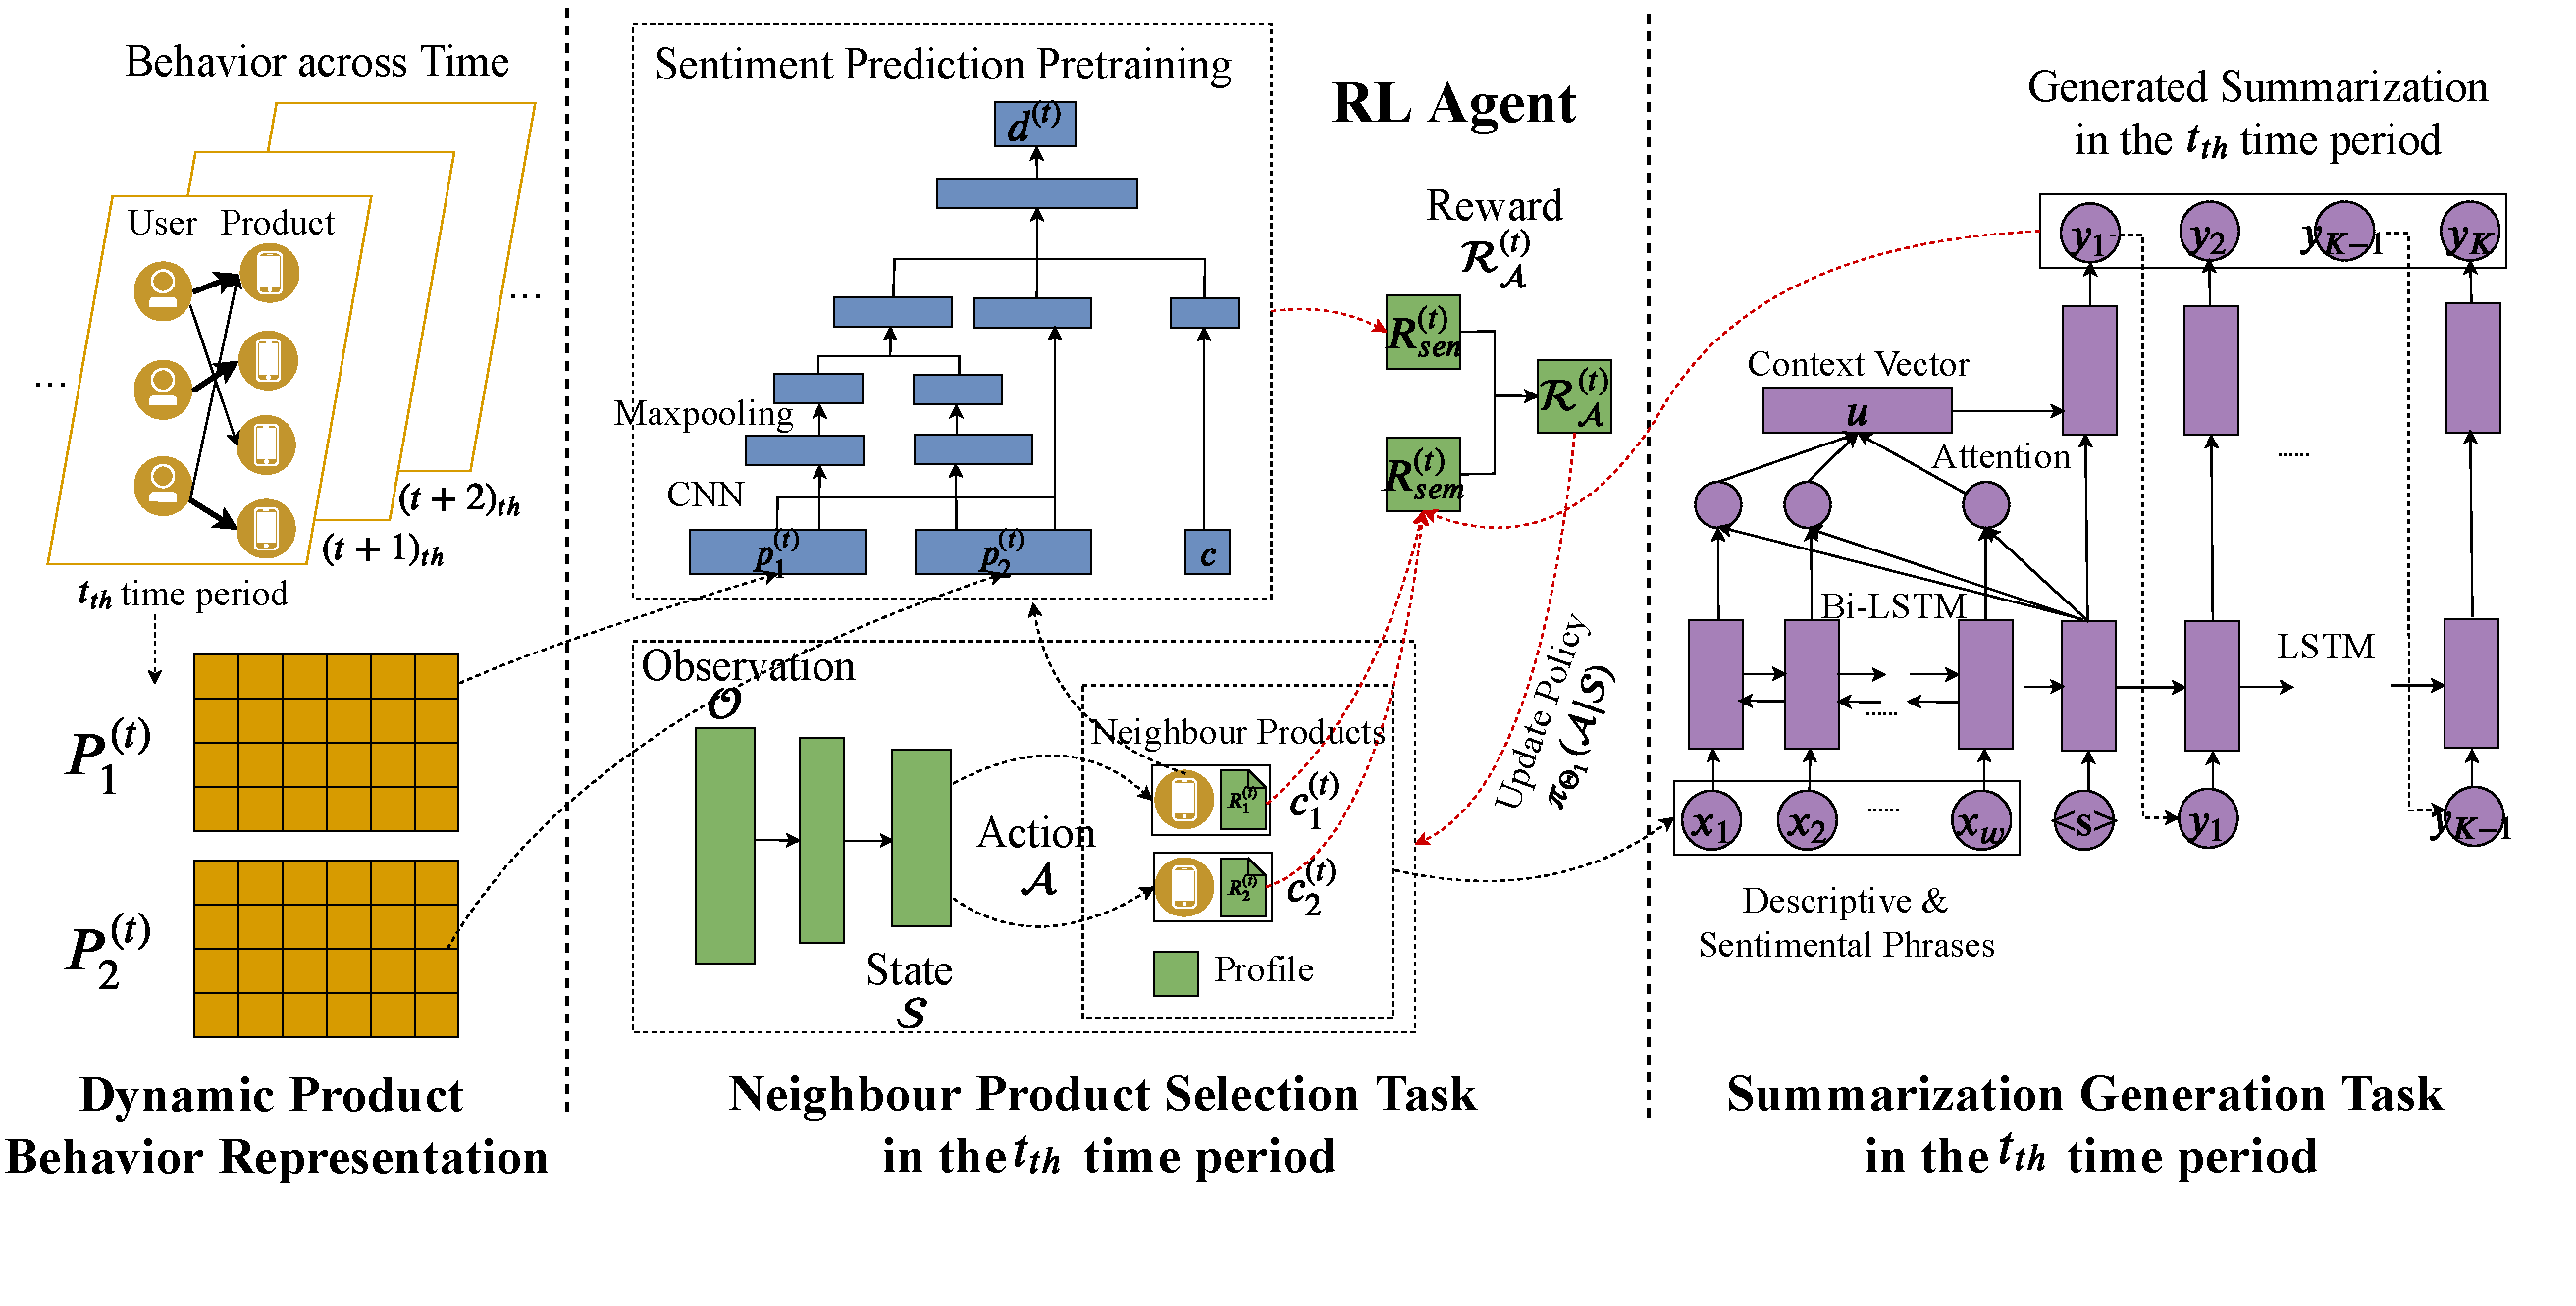
\includegraphics[width=1\textwidth]{img/chapter5/pipeline.pdf}
	\caption{ The overall architecture of BDS model in the $t_{th} $ time period. Each color refers to an individual model component. Dynamic Product Behavior Representation (for all products) and Community Distribution Pretraining (for seed products only) are optimized before training the main multi-task model (Neighbor Product Selection \& Summarization Generation). Red dashed lines show the workflows to calculate RL reward and in return to optimize RL policy. Data Prerequisite steps are omitted here for simplicity but are illustrated in detail in the main paper. }
	\label{fig:c5_pipeline}
\end{figure*}

The overall model architecture is sketched in Figure \ref{fig:c5_pipeline}. My final goal is to generate product dynamic summarizations using behavior data instead of product reviews. To optimize BDS model, the involved data are categorized into two groups: training \& validation data and seed product data. The training \& validation data contains products with both sufficient user behavior and temporal reviews in an individual time period. While seed product data are products required to have sufficient behaviors and reviews across all time periods. The training \& validation data helps to calculate dynamic product behavior presentations (\textit{Section \ref{sc:dpbr}}) and seed product data pretrains community distribution model (\textit{Section \ref{sc:spp}}). Subsequently, a multi-task model dynamically selects neighbor products (\textit{Section \ref{sc:rns}}) from seed products whose sentimental phrases filtered from reviews contribute to generate product summarization (\textit{Section \ref{sc:sgt}}). 

\subsection{Data Prerequisite} \label{sc:dp}

Before optimizing BDS model, four following types of information need to be clarified and extracted as data prerequisite:

\textbf{Seed Products:} The top products having the most sufficient behaviors and reviews across all $t$ time periods are regarded as seed products. Their community distributions are prior-known in each time period, which are later used to guide neighbor product selection (Section \ref{sc:npst}). 

\textbf{Product Descriptive Phrase:} AliNLP\footnote{English Tutorial: https://www.alibabacloud.com/help/product/57736.html \\ Chinese Tutorial: https://data.aliyun.com/product/nlp}, a paid NLP service by Alibaba, can extract name entities and sentimental phrases from E-commerce review contexts. Each product is associated with a description profile. After applying AliNLP Named Entity Recognizer (NER) on their profiles, I only keep the noun phrases to characterize related products.

\textbf{Review Sentimental Phrase:} The AliNLP sentiment analyzer can also extract sentimental phrases related to specific aspects from seed product reviews, i.e., `poor quality' is a sentimental phrases of `\textit{Quality}' aspect. Later on, these filtered sentimental phrases will be concatenated with product descriptive phrases as the model input for product summarization (Section \ref{sc:sgt}).

\textbf{Product Community Distribution:} In this paper, seed product' community distribution is prior knowledge which is learned from their reviews via AliNLP. As user behaviors has strong correlation to product characteristics, their behavior based communities should also be strongly correlated with communities calculated from product reviews which depicts product characteristics. It is a normalized vector in which each dimension represents the product affiliation towards each community, It is the ground truth to guide Community Distribution Pretraining (Section \ref{sc:spp}).  

\subsection{Dynamic Product Behavior Representation} \label{sc:dpbr}

Matrix factorization is utilized on dynamic user behaviors to learn product behavior representation across all time periods. In the initial time period, I learn both user and product $m$ types of behavior representations via related user behavior $\{B^{(0)}_{1},...,B^{(0)}_{m}\}$, where a behavior type can refer to `\textit{Click}' or `\textit{Purchase}', etc. The $i_{th}$ type of user behavior $B^{(0)}_{i}$ is in a format of sparse matrix where each row denotes a user and each column denotes a product. The data points in $B^{(0)}_{i}$ denote users' $i_{th}$ type of behaviors on products. Considering all potential methods listed in \textit{Section \ref{sc:baseline}}, I empirically select Probabilistic Matrix Factorization (PMF) to decompose $B^{(0)}_{i}$ to user representation matrix $U^{(0)}_{i}$ and product representation matrix $P^{(0)}_{i}$ by satisfying the following equation:
\begin{equation}
B^{(0)}_{i} = U^{(0)}_{i} (P^{(0)}_{i})^\intercal, i = 1,...,m
\end{equation}

As user shopping preference is consistently stable, once user representation $U^{(0)}_{i}$ is calculated from the initial period, it remains unchanged and bridges product dynamic behavior representation in subsequent time periods. 

In the $t_{th}$ time period, the matrix form of Least Squares Approximation \cite{nasrabadi2007pattern} helps to calculate the $i_{th}$ type of product behavior representation $P^{(t)}_{i}$ given related user behavior $B^{(t)}_{i}$ and user consistent representation $U^{(0)}_{i}$:
 
\begin{equation}
\begin{aligned} 
& B^{(t)}_{i} = U^{(0)}_{i} (P^{(t)}_{i})^\intercal, i = 1,...,m \\
& \Rightarrow (U^{(0)}_{i})^\intercal (B^{(t)}_{i} - U^{(0)}_{i} (P^{(t)}_{i})^\intercal) = 0 \\
& \Rightarrow (U^{(0)}_{i})^\intercal U^{(0)}_{i} (P^{(t)}_{i})^\intercal = (U^{(0)}_{i})^\intercal B^{(t)}_{i} \\ 
& \Rightarrow (P^{(t)}_{i})^\intercal = (( U^{(0)}_{i})^\intercal U^{(0)}_{i})^{-1}(U^{(0)}_{i})^\intercal B^{(t)}_{i} \\
& \Rightarrow P_{i}^{(t)} = (B_{i}^{(t)})^\intercal U^{(0)}_{i}(( U^{(0)}_{i})^\intercal U^{(0)}_{i})^{-1}
\end{aligned}
\end{equation}


\subsection{Neighbor Product Selection Task}\label{sc:npst}

\subsubsection{Community Distribution Pretraining} \label{sc:spp}

This pretraining process is only leveraged on seed products. In the $t_{th}$ time period, I combine product behavior representation and category to estimate product community distribution via a hybrid CNN-MLP (Convolutional Neural Network and Multilayer Perceptron) approach. Let $c$ be the category of a target product, stored originally as one-hot embedding. To better represent its enriched information, I first apply an one-layer MLP with $\rm tahn(\cdot)$ activation function to convert it as a dense vector $v^{c}$.

\begin{equation}
v^{c} = {\rm tahn}(W^{c}c+b^{c})
\end{equation}

where $W^{c}$ and $b^c$ denote the weight matrix and bias respectively.

For the same product, I can also obtain its multi-type behavior representation $\{p^{(t)}_{1},...,p^{(t)}_{m}\}$, where $p^{(t)}_{m} \in P^{(t)}_{m}$ denotes its $m_{th}$ type behavior representation. As CNN kernel can help to filter out the most important dimensions (local features) from a vector, a CNN layer ${\rm cnn}(\cdot)$ with Max pooling mechanism ${\rm max\_pooling}(\cdot)$ is applied to capture product $i_{th}$ type local feature representation $l^{(t)}_{i}$.
\begin{equation}
% \vspace{-0.5em}
\begin{aligned} 
&l^{(t)}_{i} = {\rm max\_pooling}({\rm tahn}({\rm cnn}(p^{(t)}_{i}))), i= 1,...,m
\end{aligned} 
\end{equation}


Subsequently, I average all $m$ types of local feature representation to a single vector $l^{(t)}$. Similarly, I calculate the average product behavior vector $p^{(t)}$ as global feature representation of $m$ types of behaviors: 
\begin{equation}
\begin{aligned} 
&l^{(t)} = \frac{1}{m}\sum_{i = 1}^{m}l^{(t)}_{i} \\
&p^{(t)} = \frac{1}{m}\sum_{i = 1}^{m}p^{(t)}_{i} 
\end{aligned} 
\end{equation}

In the end, a product has three types of information representation, including global feature representation $p^{(t)}$, local feature representation $l^{(t)}$, and category representation $v^{c}$. I concatenate all these information to calculate the estimated product community distribution $d^{(t)}$ over all pre-selected aspects via one layer MLP normalized by $\rm softmax(\cdot)$ function:
\begin{equation}
d^{(t)} = {\rm softmax}(W^{d}[p^{(t)},l^{(t)},v^{c}]+b^{d})
\end{equation}
where $W^{d}$ and $b^{d}$ are related weight matrix and bias. $[\,, ]$ denotes the concatenation operation. 

This pretraining process is optimized by minimizing the cross entropy between the estimated product community distribution $d^{(t)}$ and the actual product community distribution calculated from product reviews (Section \ref{sc:dp}). This optimization step has to be done ahead of the main multi-task model introduced in the following sections. In the later training process, for all products in the training \& validation dataset, their estimated community distribution can be calculated from the optimized pretraining model.

\subsubsection{Reinforcement Neighbor Selection} \label{sc:rns}

In the $t_{th}$ time period, among $h$ seed products with sufficient reviews, a policy gradient approach earns an action to select $s$ neighbor products $\mathcal{A} = \{\alpha_{1}^{(t)},\alpha_{2}^{(t)},...,\alpha_{s}^{(t)}\}$ out of $h$ candidates where $\alpha_{s}^{(t)}$ denotes the $s_{th}$ selected neighbor product. As I do not consider the sampling sequence on neighbor products, the reinforcement approach is a one-step Markov Decision Process (MDP) with single state $\mathcal{S}$ and single action $\mathcal{A}$. 

Assume there are $n$ products in total across all time periods, given a target product, the initial observation $\mathcal{O}$ is the product itself, represented as a one-hot embedding $\in \mathbb{R}^{n}$. The state $\mathcal{S}$ is learned via a two-layer Multilayer Perception (MLP) on the initial observation $\mathcal{O}$:
\begin{equation}
\label{eq:state}
\mathcal{S} = {\rm softmax} (W_{2}{\rm tahn}(W_{1}\mathcal{O} + b_{1}))
\end{equation} 
where $W_1$,$W_2$ and $b_1$ denote related weight matrices and bias, respectively. 

The learned state $\mathcal{S} \in \mathbb{R}^{h}$ is the selection probability distribution over $h$ seed products. Assuming an action is taken to sample $s$ neighbor products with related probability weights $\{\omega_{1}^{(t)},\omega_{2}^{(t)},...,\omega_{s}^{(t)}\} \in \mathcal{S}$, the sampling policy $\pi_{\Theta_{1}}(\mathcal{A}|\mathcal{S})$ can be therefore calculated as:
\begin{equation}
\pi_{\Theta_{1}}(\mathcal{A}|\mathcal{S}) = s!\prod_{i=1}^{s}\omega^{(t)}_{i}
\end{equation} 
$\Theta_{1}$ denote the parameters to be learned. The factorial of $s$ ($s!$) denotes the number of permutations for the selected neighbor products as the neighbor products are sequence insensitive. $\prod_{i=1}^{s}\omega^{(t)}_{i}$ is the generative probability of each permutation. 

To assess the fitness of the $s$ selected neighbor products for the target product, I design two dynamic rewards: a community reward to measure the community similarity, and a semantic reward to calculate the content similarity between $s$ neighbor products and the target product.

\textbf{Community Reward:} 
In the $t_{th}$ time period, I estimate the target product's community distribution as $d^{(t)}_{a}$ by the Community Distribution Pretraining (Section \ref{sc:spp}). The community distributions of all its selected neighbor products $\{d^{(t)}_{1},...,d^{(t)}_{s}\}$ are known as prior knowledge (Section \ref{sc:dp}). To evaluate pairwise distribution similarity, Pearson correlation calculates the community reward $ \mathcal{R}_{com,i}^{(t)}$ of the $i_{th}$ selected neighbor product $\alpha_{i}^{(t)}$ as follows:

\begin{equation}
\mathcal{R}_{com,i}^{(t)} = \frac{\mathbb{E}[(d_{a}^{(t)}-\mu(d_{a}^{(t)}))(d_{i}^{(t)}-\mu(d_{i}^{(t)}))]}{\sigma(d_{a}^{(t)})\sigma(d_{i}^{(t)})}, i = 1,...,s
\end{equation}

where $\mathbb{E}(\cdot)$ denotes the expectation, $\mu(\cdot)$ denotes the mean and $\sigma(\cdot)$ denotes the standard deviation. Larger similarity score offers a higher reward to the related neighbor product.

\textbf{Semantic Reward:} In the $t_{th}$ time period, the semantic reward of neighbor products is measured by the accuracy of generated product summarization. In this paper, we use the word level Jaccard Similarity as the indicator to calculate the semantic reward $\mathcal{R}_{sem}^{(t)}$ for all selected neighbor products, which contains two parts: the averaged Jaccard Similarity between all neighbor product original reviews and real product summarization, and the Jaccard Similarity between generated product summarization and actual product summarization:

\begin{equation}
\mathcal{R}_{sem}^{(t)} = \frac{1}{s}\sum_{i=1}^{s} \frac{|R_{i}^{(t)} \cap Y^{(t)}|}{|R_{i}^{(t)} \cup Y^{(t)}|} + \frac{|\hat{Y}^{(t)} \cap Y^{(t)}|}{|\hat{Y}^{(t)} \cup Y^{(t)}|} 
\end{equation}

where $R_{i}^{(t)}$ denotes all original reviews of the $i_{th}$ neighbor product $\alpha_{i}^{(t)}$, $\hat{Y}^{(t)}$ denotes the generated summarization of target product, and $Y^{(t)}$ denotes its actual summarization. The total reward $\mathcal{R}^{(t)}_{\mathcal{A}}$ of neighbor products is the weighted sum between community reward and semantic reward controlled by a weighting factor $\gamma$:


\begin{equation}
\mathcal{R}^{(t)}_{\mathcal{A}} = \sum_{i=1}^{s} \omega_{i}^{(t)}\mathcal{R}_{com,i}^{(t)} +\gamma \mathcal{R}_{sem}^{(t)}
\end{equation}

\textbf{Task Optimization:} I use policy gradient method to optimize the sampling policy, aiming to maximize the expected total reward for neighbor products. The expected reward $\mathcal{J}_{sel}(\Theta_{1})$ in the $t_{th}$ time period is:

\begin{equation}
\begin{aligned}
\mathcal{J}_{sel}(\Theta_{1}) &= \mathbb{E}_{\mathcal{A} \sim \pi_{\Theta_{1}}(\mathcal{A}|\mathcal{S})}[\mathcal{R}^{(t)}_{\mathcal{A}}]
\end{aligned}
\end{equation}

Then, the gradient is estimated using the likelihood ratio trick:

\begin{equation}
\label{eq:loss_1}
\begin{aligned}
\nabla_{\Theta_{1}}\mathcal{J}_{sel}(\Theta_{1}) &= \nabla_{\Theta_{1}} \sum_{\mathcal{A}} \pi_{\Theta_{1}}(\mathcal{A}|\mathcal{S}) \mathcal{R}^{(t)}_{\mathcal{A}}\\
&\approx \frac{1}{N} \sum_{i=1}^{N}\nabla_{\Theta_{1}}log\pi_{\Theta_{1}}(\mathcal{A}_{i}|\mathcal{S})\mathcal{R}^{(t)}_{\mathcal{A}_{i}}
\end{aligned}
\end{equation}

where $\mathcal{A}_{i}$ denotes the $i_{th}$ of $N$ randomly sampled actions (selecting $s$ neighbor products from $h$ seed products). 

\subsection{Summarization Generation Task} \label{sc:sgt}

In the $t_{th}$ time period, the filtered neighbor product sentimental phrases together with product own descriptive phrases are concatenated into a sequence $X^{(t)} = \{x_{1},...,x_{w}\}$. It is used as the input of Neural Machine Translation (NMT) model to generate product summarization sequence $Y^{(t)} = \{y_{1},...,y_{k}\}$. $w$ and $k$ denote the input and output sequence length, respectively. Filtering out most of emotional and other irrelevant words in advance can better map the input to aspect oriented summarizations instead of subjective review summaries. 

The input sequence $X^{(t)} = \{x_{1},...,x_{w}\}$ is fed one-by-one into the encoder (a single-layer bidirectional LSTM), producing a sequence of encoder hidden states $\{e_{1},...,e_{w}\}$. In decoding step $i$, the decoder (a single-layer unidirectional LSTM) has a decoder hidden state $h_{i}$. Its context vector $u_{i}$ is generated via an Attention mechanism on all encoder hidden states and current decoder hidden state:

\begin{equation}
\begin{aligned}
& a_{ij} = {\rm attention}(h_{i},e_{j}), j = 1,...,w \\
& a_{ij}^{*} = \frac{{\rm exp}(a_{ij})}{\sum_{k=1}^{w} {\rm exp}(a_{ik})}\\
& u_{i} = \sum_{j=1}^{w}a_{ij}^{*}e_{j}
\end{aligned}
\end{equation}
where $a_{ij}$ denotes the attention weight of encoder hidden state $e_{j}$. $a_{ij}^{*}$ is the normalized weight by Softmax function. The weighted sum of all encoder hidden states, $u_{i}$, is the context vector for current step $i$, reflecting the auxiliary information from input sequences.

A one-layer MLP is subsequently utilized on the combination of context vector $u_{i}$ and decoder hidden state $h_{i}$ to generate the vocabulary probability distribution $P_{vocab}$:

\begin{equation}
P_{vocab} = {\rm softmax}(W^{o}[u_{i},h_{i}]+b^{o})
\end{equation}
where $W^{o}$ and $b^{o}$ are related weight and bias.

In decoding step $i$, the generation loss for target word $y_{i}$ is its negative log likelihood, $-logP_{vocab}(y_{i})$. The overall generation loss $\mathcal{J}_{gen}(\Theta_{2})$ is the average of all $k$ step generation losses and $\Theta_{2}$ are all related parameters to be optimized.

\begin{equation}
\mathcal{J}_{gen}(\Theta_{2}) = \frac{1}{k}\sum_{i=1}^{k} -logP_{vocab}(y_{i})
\end{equation}

In the multi-task model, $\mathcal{J}_{sel}(\Theta_{1})$ and $\mathcal{J}_{gen}(\Theta_{2})$ both need to be minimized during the model training process. Each task is learned separately and alternately after taking a certain number of training data batches in their optimization processes.
\section{Experiments} \label{sc:exp} 
\subsection{Dataset}
From \textit{Taobao}, a world-leading E-commerce website owned by Alibaba, we collect user behavior and product reviews during the period from Apr/12/2018 to Jul/10/2018.the raw dataset is split into two parts: the first two-week data, as the initial time period $t_0$, helps to generate user consistent shopping preference (\textit{Section \ref{sc:dpbr}}). For the rest data, we empirically set fifteen days as the time window to split it evenly into five consecutive time periods ($t_{1} \sim t_{5}$). In each time period, four types of information need to be prepared and calculated in advance to support model training, including multi-type user behavior, product profile, product community distribution, and product ground truth summarization: 

\textbf{First}, multi-type user behavior is used for generating dynamic product behavior representation (\textit{Section \ref{sc:dpbr}}). Three types of user behavior are considered in this paper including `\textit{Click}', `\textit{Add Cart}' and `\textit{Purchase}'.

\textbf{Second}, from product profile, product category is encoded as one-hot embedding for sentiment distribution prediction (\textit{Section \ref{sc:npst}}). Descriptive phrases are extracted from product description profiles to support aspect summarization generation (\textit{Section \ref{sc:sgt}}). 

\textbf{Third}, product community distribution is calculated from reviews  by considering textual content in four common aspects including `\textit{Quality}', `\textit{Cost-performance Ratio}', `\textit{Fitness}' and `\textit{Material}'.

\textbf{Fourth}, in \textit{Taobao}, a user can rate reviews with thumbs-up or thumbs-down signal. For each product in the training data, we firstly select its top ten reviews relevant to the four picked aspects and with the largest number of thumbs-ups. After that, using AliNLP sentiment analyzer, we can locate and filter out the aspect-related sentences from the reviews as the ground truth for summarization generation (\textit{Section \ref{sc:sgt}}).  

In total, the whole dataset contains 125,598 products, 51,366 users and 108,749,788 multi-type behaviors. We use 80\% of the data for training, 10\% for validation and 10\% for testing.  


\subsection{Baselines and Settings} \label{sc:baseline}

As the main contribution of this paper lies in the reinforcement neighbor product selection task, five baselines are chosen to compare from neighbor product selection viewpoint. \textbf{1) Title Similarity} (TS): Neighbor products are selected with the shortest Levenshtein Distance on titles. \textbf{2) Random}: Neighbor products are randomly selected. \textbf{3) PMF}: PMF \cite{mnih2008probabilistic}  firstly learns product embeddings via matrix factorization. Neighbor products are selected with the highest cosine similarity score on product embeddings. \textbf{4) GBPR}: GBPR \cite{pan2013gbpr} uses a Bayesian based collaborative filtering method to assign user preferences on products. Neighbor products are selected with the most similar user preferences. \textbf{5) EALS}: EALS \cite{he2016fast} is a fast matrix factorization approach which learns product embeddings. Neighbor products are selected with the highest cosine similarity score on product embeddings. After the neighbor products are selected, their reviews' sentimental phrases together with product own descriptive phrases are utilized to generate product summarization via the same NMT model struture  as our BDS model. We intentionally apply the same generative model so as to compare the effectiveness of neighbor products selection in different models.

To assess the usefulness of neighbor product information, our model is compared with another two generative models only leveraging product own  metadata. \textbf{6) Raw Title} (RT) uses the product titles and  \textbf{7) Title-Review} (TR) uses the concatenation of product title and sparse reviews as the input of the same NMT model to generate aspect summarization.
 

Mini-batch (\textit{size = 20}) Adam SGD optimizer is used to train our model for 100 epochs. Learning rate is 0.01. Dimension of product \& user representation is 300 (\textit{Section \ref{sc:dpbr}}). $s=5$ neighbor products are selected from $h=100$ seed products (\textit{Section \ref{sc:npst}}). Vocabulary size in summarization generation (\textit{Section \ref{sc:sgt}}) is \textit{15K}. Other parameter details will be offered once the paper gets published.


\subsection{Evaluation Metrics}
In this paper, we report the model performance via the following metrics from both automatic and human perspectives. Automatic metrics evaluate the accuracy of the generated summarizations by objectively calculating the correctness of predicted words. While human metrics evaluate the semantic quality of generated summarizations by subjectively considering their sentence readability. 
\begin{itemize}
	\item \textbf{ROUGE} (RG)\footnote{https://pypi.org/project/pyrouge/}
	: evaluates text summarization quality by comparing the overlap between generated sequences and the ground truth. We report RG-1, RG-2 and RG-L in this paper.
	\item \textbf{METEOR}\footnote{http://www.cs.cmu.edu/~alavie/METEOR/}
	: is the harmonic mean of generated summarizations' unigram precision and recall. It offers stemming and synonymy matching along with standard exact word matching.
	
	\item \textbf{Human Evaluation}: We generate summaries of 200 random products by each of the seven baselines and our model. To compare BDS model with each baseline, three human votes are collected from a crowd-sourcing platform for each pair of product summaries ($200*7*3 = 4,200$ human judgements). People are required to vote the one with more comprehensive information and better sentence structure. We define \textit{winning time rate} (WTR) and \textit{winning count rate}  (WCR) as two human evaluation metrics. Given a pair of model $A$ and model $B$, the WTR of $A$ is the ratio of winning products for $A$ and the WCR of $A$ is the ratio of winning votes for $A$. For instance, given two products $\alpha$ and $\beta$, if method $A$ gets two votes for $\alpha$ and one vote for $\beta$, its WTR is $(1+0)/(1+1)=0.5$ and WCR is $(2+1)/(3+3)=0.5$.
\end{itemize}

\section{Discussion}
As neighbour product selection (Task 1) is an unsupervised approach whose ultimate goal is to support product summarization (Task 2),  I only report the experimental results on Task 2 to demonstrate my model's superiority over the baselines across different timestamps. The efficacy of each input component is also presented here.

\subsection{Automatic Evaluation}

I run my model ten times and report the average evaluation results in the left part of Table \ref{tab:auto-eval}. To verify my model's superiority, I calculate the performance differences between my model and each baseline on each automatic metric for all the ten runs, and apply a t-test on the ten differences to check whether the performance difference is significant. 

RT performs the worst as the product title contains limited and static information to reveal product sentiment dynamics. From TR results, adding sparse reviews can improve model performance, but is still worse than the rest approaches, which strongly indicates the effectiveness of using neighbour product reviews for generating aspect summarization. Most of neighbour selection based baselines have roughly similar results except TS model, meaning that behavior based is better than content based neighbour selection. Surprisingly, Random model can achieve a relatively satisfying result. One possible reason is that because most of reviews in online shopping websites are positive, randomly sampled neighbour product might receive reviews containing relevant sentimental phrases. Howsoever, my BDS model outperforms all baselines significantly (\textit{p$<$0.01}) on all metrics, demonstrating the superiority of my proposed reinforcement neighbour selection.
 

\begin{table}
	% \scriptsize
	
%	\small
	\centering
%	\renewcommand{\tabcolsep}{3pt}
	
	\begin{tabular}{ccccccc} 
		\toprule
		\multirow{2}{*}{ \textbf{Model}}&  \multicolumn{4}{c}{\textbf{Automatic}} & \multicolumn{2}{c}{\textbf{Human }}\\ \cmidrule(lr){2-7}
		&RG-1&RG-2&RG-L&METEOR &WTR &WCR \\ \midrule 
		RT &  36.19 & 10.01 & 27.95 & 16.05& 0.00&0.01\\ 
		TR& 43.05  & 19.08 &  33.10  & 19.24 & 0.07&0.13 \\ 
		TS & 42.97  & 18.85  & 32.85  & 19.34 &0.13 &0.24 \\ 
		Random& 44.21 &  19.58 &  33.98  &  19.86 &0.03 &0.13\\ 
		PMF & 45.72 &  20.25  &  35.21  & 20.80 &0.14 & 0.28\\ 
		GBPR& 45.09 &  19.67  &  34.55&  20.36 & 0.32&0.39\\ 
		EALS& 44.66  & 19.50  &  34.28 &    20.32&0.08 &0.17\\ 
		BDS& \textbf{51.11*} & \textbf{23.55*}& \textbf{39.86*} &  \textbf{22.99* }&  \textbf{0.89 }& \textbf{0.81 }\\ \bottomrule
	\end{tabular}
	% \vspace{-0.5em} 
	\caption{Automatic \& human evaluation results of my model compared with baselines. Symbol ‘*’ highlights the cases where my model significantly beats all baselines with $p$ value smaller than 0.01.}
	\label{tab:auto-eval}
	% \vspace{-1em} 
\end{table} 
 
\subsection{Human Evaluation}
The right part of Table \ref{tab:auto-eval} reports the human evaluation result for all the models. Higher WTR and WCR scores indicate the related model can generate better structured summaries from human perspective. For each baseline, WTR and WCR scores are the pairwise comparison results with the BDS model. RT model performs the worst.  And content based methods (RT and TR) also perform worse than neighbour selection based methods in general. GBPR performs much better than the rest baselines. It beats my model in roughly 30\% of summary pairs.  The reported two scores of my model are the average of pairwise comparison results with all baselines, which shows that my model can beat other baselines on 90\% of all summary pairs.

Both automatic and human evaluation results demonstrate content based baselines perform worse than neighbour selection based baselines. However, there are still some inconsistencies between their evaluation results. Although GBPR has similar performance with the rest of neighbour based baselines on automatic metrics, it unexpectedly outperforms on human metrics, which indicates how to organize sequences has huge impact on summary semantic quality.

\subsection{Dynamic Performance} 
\begin{figure} 
	\centering 
	\subfloat[ROUGE-1]{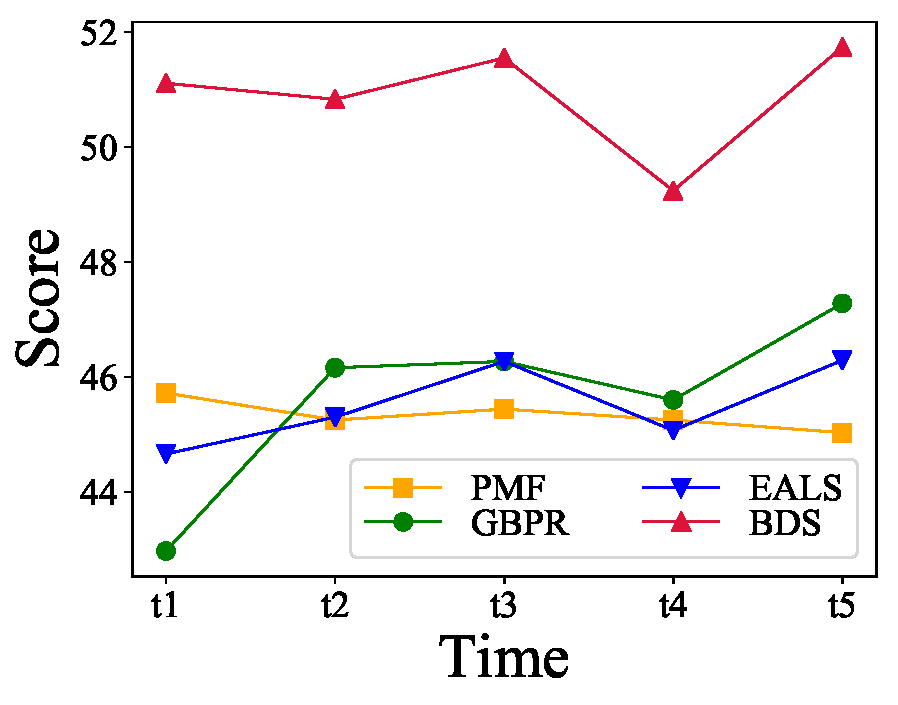
\includegraphics[width = 0.5\columnwidth]{img/chapter5/rouge-1.pdf}}
	\subfloat[ROUGE-2]{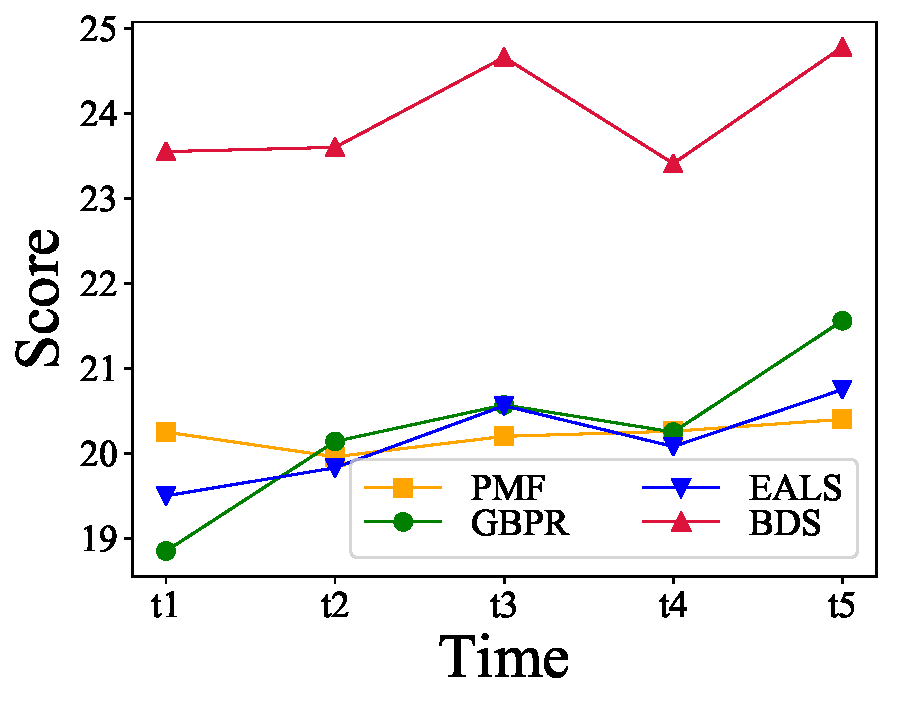
\includegraphics[width =0.5\columnwidth]{img/chapter5/rouge-2.pdf}}\\ 
	\subfloat[ROUGE-L]{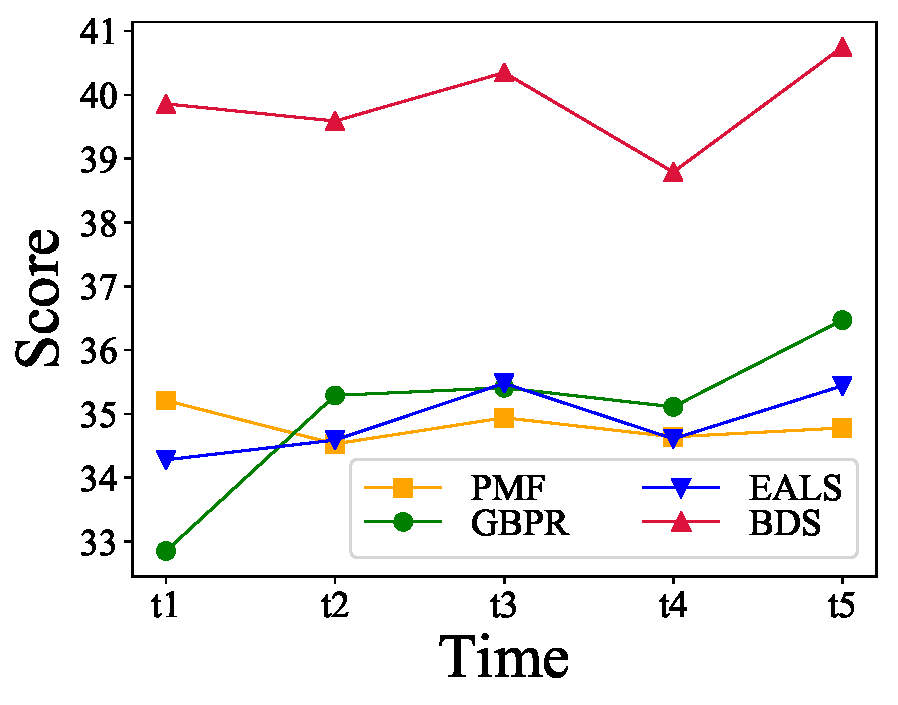
\includegraphics[width = 0.5\columnwidth]{img/chapter5/rouge-L.pdf}}
	\subfloat[METEOR]{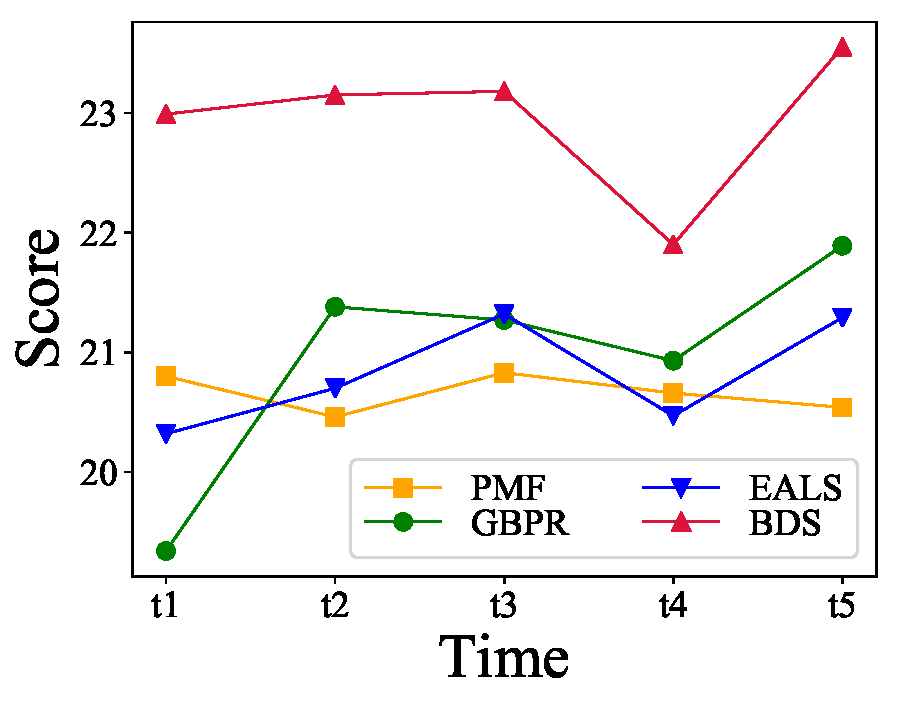
\includegraphics[width = 0.5\columnwidth]{img/chapter5/meteor.pdf}} 
	\caption{Automatic evaluation results of my model compared with the Top 3 baselines in five consecutive time periods ($t_1 \sim t_5$).} 
	\label{fig:auto-eval} 
\end{figure}
To better present my model dynamic performance, I visualize the automatic evaluation results of my model as well as  the best three baselines (PMF, EALS and GBPR) in all five consecutive time periods, shown in Figure \ref{fig:auto-eval}. The three best baselines are all neighbour selection approaches. Across all time periods, all four model performances are relatively consistent and follow similar trend. Their performances go down a little bit in the fourth time period but raise up immediately in the next time period. Among three baselines, GBPR achieves the best performance result over the rest two. It does not perform well in the beginning, but keeps growing and beats the rest baselines in later time periods. In general, the performances of three baselines are not far away from each other, especially from time period $t_2$ to $t_4$. Shown in Figure \ref{fig:auto-eval}, their plotted lines are basically mingled together. However, my model achieves a far better evaluation result than baselines. Its plotted lines (red lines) are always significantly above the rest three lines in terms of all four evaluation metrics. Moreover, model performances on the four reported metrics are with similar trend. And the three ROUGE based metrics are with an even more similar trend than METEOR. 




\subsection{Input Component Evaluation}


As aforementioned, my model requires three types of product input information: user behavior, product category, and profile descriptive phrases. To examine whether all involved information are effective, I conduct an extensive study by removing each type of information iteratively while holding the rest information fixed. Table \ref{tab:ablation} shows the performance difference between the models with truncated input and original BDS model. In detail, removing user behavior (product category) means that only product category (user behavior) is used for sentiment prediction pretraining. Removing product profiles means that only neighbour product sentimental phrases contribute to summarization generation. 
 
\begin{table}%[h]
	% \scriptsize
%	\small
	\centering
%	\renewcommand{\tabcolsep}{7pt}
	\begin{tabular}{ccccc} 
		\toprule
		
		\textbf{Model}& \textbf{RG-1} & \textbf{RG-2} & \textbf{RG-L} & \textbf{METEOR}\\ \midrule  
		-- Behavior &-14.21 & -12.63&-11.37  & -5.72\\  
		-- Category&-4.74 & -2.94&-4.27 & -1.65 \\
		-- Profile &-5.78 & -3.77&-5.33& -2.34\\  
		\bottomrule
	\end{tabular} 
	\caption{Performance differences between the model with truncated input and original BDS model. `--' means removing related input component from my model.}
	\label{tab:c5_ablation} 
\end{table}
From Table \ref{tab:c5_ablation}, removing related input component always leads a decrease on model performance, which indicates that all the three types of input component are useful in BDS model. Compared with product category and descriptive phrases, user behavior obviously has the most influential impact because removing it causes the largest drop in model performance over all four reported metrics. Surprisingly, it declines the model performance down close to the worst baseline, RT. It explicitly verifies the importance of user behavior for product summarization generation. Moreover, the performance decrease by removing profile descriptive phrases is larger than removing product category embedding. The reason might be that profile descriptive phrases are directly used for summarization generation. While product category contributes to the sentiment prediction pretraining, which only has implicit impact and is not able to directly reflect dynamic aspect sentiment changes. 
 
\subsection{Case Study} 
\begin{table}%[h]
%	\scriptsize
	% \small
	\centering
%	\renewcommand{\tabcolsep}{3pt} 
%	\renewcommand\arraystretch{0}
	
	
	\begin{tabular}{p{1cm}p{6cm}p{6cm}} 
		\toprule
		
		\textbf{Time} & \multicolumn{1}{c}{\textbf{Ground Truth}} & \multicolumn{1}{c}{\textbf{BDS}}\\ \midrule 
		$t_1$ & \colorbox{YellowGreen}{\textbf{Material : Positive}} \newline \textbf{Summarization:} The \textcolor{YellowGreen}{\textbf{material}} of the dress is super \textcolor{YellowGreen}{\textbf{nice}} and  \textcolor{YellowGreen}{\textbf{soft to wear}}. It is made of cotton and touches like a   \textcolor{YellowGreen}{\textbf{high-end}} dress. A perfect gift for aged women. & \colorbox{YellowGreen}{\textbf{Material : Positive }} \newline \textbf{Summarization:} The dress has \textcolor{YellowGreen}{\textbf{good material }}. It is made of \textcolor{YellowGreen}{\textbf{cotton and touches very soft}}. A perfect gift for mums who have \textcolor{YellowGreen}{\textbf{high-standard}} requirement on dress material.\\ \midrule 
		$t_2$ & \colorbox{red}{\textbf{Material : Negative }} \newline \textbf{Summarization:} The dress \textcolor{red}{\textbf{material}} is \textcolor{red}{\textbf{not as good as promised}}. It is \textcolor{red}{\textbf{not good}} for aged women with high requirements. It touches as \textcolor{red}{\textbf{cheap material}} and smells weird. & \colorbox{red}{\textbf{Material : Negative }} \newline \textbf{Summarization:} The \textcolor{red}{\textbf{material is terrible}}. It touches like \textcolor{red}{\textbf{carded yarn with much cheaper material}} as promised for mums. It has a weird smell when wearing it. \\ \bottomrule
	\end{tabular}   
	\caption{A real case to show my model's generated dynamic sentiment summarization for a dress on product material. The \textcolor{YellowGreen}{green} color indicates positive words. While \textcolor{red}{red} color indicates negative words.}
	
	\label{tab:c5_demo} 
\end{table} 
We conduct a case study in Table \ref{tab:c5_demo} on an actual dress to show how my model summarize its aspect-sentiment changes in a timely manner. In this case, I only care about sentiment changes on product material and demonstrate material-related content from the full generated summaries. In the real world, the sentiment of the dress material goes from positive to negative (concluded from summarization) due to its manufacturer's counterfeit (reported by customers in time $t_2$). My model is able to  detect this aspect-sentiment change from its updated customer shopping behaviors and dynamically locate neighbour products with similar issues (like material problems). From the result shown in Table \ref{tab:c5_demo}, the generated summaries on `Material' aspect supports my model effectiveness. Moreover, the generated summaries solely contain objective descriptions instead of emotional expressions used in personal reviews, which shows a  more formal and aspect-concentrated way of description than summarized reviews. 






%%%%%%%%%%%%%%%%
% Chapter 6
%%%%%%%%%%%%%%%%

%\chapter{Conclusion}
\section{Contributions}
\section{Limitation}
Existing methods limitation: \cite{lancichinetti2011limits},\cite{kawamoto2015limitations},\cite{xiang2012multi},\cite{aldecoa2013exploring} ,\cite{xiang2012limitation}, 
\section{Future Work} 






%%%%%%%%%%%%%%%%
% Appendices
%%%%%%%%%%%%%%%%

%\begin{appendices}

%Some Table of Contents entry formatting
\addtocontents{toc}{\protect\renewcommand{\protect\cftchappresnum}{\appendixname\space}}
\addtocontents{toc}{\protect\renewcommand{\protect\cftchapnumwidth}{6em}}

%Begin individual appendices, separated as chapters

\chapter{Experimental Equipment}
Lorem ipsum dolor sit amet, consectetur adipiscing elit, sed do eiusmod tempor incididunt ut labore et dolore magna aliqua. Ut enim ad minim veniam, quis nostrud exercitation ullamco laboris nisi ut aliquip ex ea commodo consequat. Duis aute irure dolor in reprehenderit in voluptate velit esse cillum dolore eu fugiat nulla pariatur. Excepteur sint occaecat cupidatat non proident, sunt in culpa qui officia deserunt mollit anim id est laborum.

\chapter{Data Processing}
Lorem ipsum dolor sit amet, consectetur adipiscing elit, sed do eiusmod tempor incididunt ut labore et dolore magna aliqua. Ut enim ad minim veniam, quis nostrud exercitation ullamco laboris nisi ut aliquip ex ea commodo consequat. Duis aute irure dolor in reprehenderit in voluptate velit esse cillum dolore eu fugiat nulla pariatur. Excepteur sint occaecat cupidatat non proident, sunt in culpa qui officia deserunt mollit anim id est laborum.

\end{appendices}

%%%%%%%%%%%%%%%%
% References
%%%%%%%%%%%%%%%%
%\begin{singlespace}  % use single-line spacing for multi-line text within a single reference
%	\setlength\bibitemsep{\baselineskip}  %manually set separataion betwen items in bibliography to double space
%	\printbibliography[heading=bibintoc,title={References}]
%\end{singlespace}
\printbibliography[heading=bibintoc,title={References}]
%\addcontentsline{toc}{chapter}{References}  %add References section to Table of Contents

%%%%%%%%%%%%%%%%
% Vita 
% Only for PhD students
% Masters students remove this line
%%%%%%%%%%%%%%%%
\chapter*{Curriculum Vitae}
\addtocontents{toc}{
 \unexpanded{\unexpanded{\renewcommand{\cftchapdotsep}{\cftnodots}}}%  
}
\pagenumbering{gobble}
\addcontentsline{toc}{chapter}{Curriculum Vitae} 
%\doublespacing
\begin{spacing}{1.0}
	%%行间距变为single-space


\begin{cv}{}
	\begin{cvlist}{Education}
		\item[08/2015--06/2020] \textbf{Ph.D. in Information Science} \\ Indiana University Bloomington, USA
		\item[08/2013--05/2015] \textbf{Master in Information Science}\\ University of Pittsburgh, USA
		\item[08/2009--05/2013] \textbf{Bachelor in Information Management and System} \\ Shanghai International Studies University, China
	\end{cvlist}

	\begin{cvlist}{Industry Experience}
	\item[06/2019--09/2019] Data Scientist Intern, Amazon Alexa AI, USA 
	\item[02/2018--03/2019] NLP research Intern, Alibaba DAMO Academy, China
	\end{cvlist}

	\begin{cvlist}{Teaching Experience}
		\item[01/2018--12/2019] Instructor / Lecturer, Indiana University Bloomington, USA
	\item[08/2015--12/2017] Associate Instructor, Indiana University Bloomington, USA
	\end{cvlist}
	
	\begin{cvlist}{Publication}
		\item \textbf{Zheng Gao}, Hongsong Li, Zhuoren Jiang, Xiaozhong Liu. Detecting User Community in Sparse Domain via Cross-Graph Pairwise Learning. \textit{ACM SIGIR Conference on Research and Development in Information Retrieval (SIGIR)}, 2020.
		 \item \textbf{Zheng Gao}, Lujun Zhao, Heng Huang, Hongsong Li, Changlong Sun, Luo Si, Xiaozhong Liu. Behavior based Dynamic Summarization on Product Aspects via Reinforcement Neighbour Selection. \textit{European Conference on Artificial Intelligence (ECAI)}, 2020.
		\item Zhuoren Jiang, \textbf{Zheng Gao}, Jinjiong Lan, Hongxia Yang, Yao Lu and Xiaozhong Liu. Task-Oriented Genetic Activation for Large-Scale Complex Heterogeneous Graph Embedding. \textit{The Web Conference (WWW)}, 2020.
		\item \textbf{Zheng Gao}, Chun Guo, Xiaozhong Liu. Efficient Personalized Community Detection via Genetic Evolution. \textit{The Genetic and Evolutionary Computation Conference (GECCO)}, 2019.
		\item \textbf{Zheng Gao}, Gang Fu, Chunping Ouyang, Satoshi Tsutsui, Xiaozhong Liu, Jeremy Yang, Christopher Gessner, Brian Foote, David Wild, Ying Ding, Qi Yu. edge2vec: Representation Learning Using Edge Semantics for Biomedical Knowledge Discovery. \textit{BMC Bioinformatics}, 2019. (impact factor = 2.511).
		\item Yongzhen Wang, Xiaozhong Liu, \textbf{Zheng Gao}. Neural Related Work Summarization with a Joint Context-driven Attention Mechanism. \textit{Conference on Empirical Methods in Natural Language Processing (EMNLP)}, 2018.
		\item Zizhe Gao, \textbf{Zheng Gao}, Heng Huang, Zhuoren Jiang, Yuliang Yan. An End-to-end Model of Predicting Diverse Ranking On Heterogeneous Feeds. \textit{eCOM Workshop at ACM SIGIR Conference on Research and Development in Information Retrieval (eCom-SIGIR)}, 2018.
		\item \textbf{Zheng Gao}, Lin Guo, Chi Ma, Xiao Ma, Kai Sun, Hang Xiang, Xiaoqiang Zhu, Hongsong Li, Xiaozhong Liu. AMAD: Adversarial Multiscale Anomaly Detection on High-Dimensional and Time-Evolving Categorical Data. \textit{Deep Learning Practice for High-Dimensional Sparse Data Workshop at ACM SIGKDD Conference on Knowledge Discovery and Data Mining (DLP-KDD)}, 2019.
		\item Zhuoren Jiang, Liangcai Gao, Ke Yuan, \textbf{Zheng Gao}, Zhi Tang, Xiaozhong Liu. Mathematics Content Understanding for Cyberlearning via Formula Evolution Map. \textit{ACM International Conference on Information and Knowledge Management (CIKM)}, 2018.
		\item Xiaozhong Liu, Xing Yu, \textbf{Zheng Gao}, Tian Xia, Johan Bollen. Comparing Community-based Information Adoption and Diffusion across Different Microblogging Sites. \textit{ACM Conference on Hypertext and Social Media}, 2016.
		\item \textbf{Zheng Gao}, Vincent Malic, Shutian Ma, Patrick Shih. How to Make a Successful Movie: Factor Analysis from both Financial and Critical Perspectives. \textit{International Conference on Information}, 2019.
		\item Yongzhen Wang, Yan Lin, \textbf{Zheng Gao}, Yan Chen. A Two-stage Iterative Approach to Improve Crowdsourcing-based Relevance Assessment. \textit{Arabian Journal for Science and Engineering}, 2019.
		\item \textbf{Zheng Gao}, John Wolohan, Fast NLP-based Pattern Matching in Real Time Tweet Recommendation. \textit{Text REtrieval Conference (TREC)}, 2017.
		\item \textbf{Zheng Gao}, Rui Bi. University of Pittsburgh at TREC 2014 Microblog Track. 
		\textit{Text REtrieval Conference (TREC)}, 2014.
		\item \textbf{Zheng Gao}, Xiaozhong Liu. Personalized Community Detection in Scholarly Network. \textit{International Conference on Information}, 2017.
		\item Tian Xia, Xing Yu, \textbf{Zheng Gao}, Yijun Gu, Xiaozhong Liu. Internal/External Information Access and Information Diffusion in Social Media. \textit{International Conference on Information}, 2017.
		\item Nan Li, Naren Suri, \textbf{Zheng Gao}, Tian Xia, Xiaozhong Liu, Katy Borner. Enter a Job, Get Course Recommendations. \textit{International Conference on Information}, 2017.
		
		\item Chenwei Zhang, \textbf{Zheng Gao}, Xiaozhong Liu. How Others Affect Your Twitter \#hashtag Adoption? Examination of Community-based and Context-based Information Diffusion in Twitter. \textit{International Conference on Information}, 2015. 
		\item \textbf{Zheng Gao}, Patrick C. Shih. Communities of Support: Social Support Discussion in a HIV Online Forum. \textit{International Symposium of Chinese CHI}, 2019.
		\item Satoshi Tsutsui, \textbf{Zheng Gao}, Yuzhuo Wang, Guilin Meng, Ying Ding. A Case Study on Viziometrics: What’s the Role of Western Blots in Alzheimer’s Disease Literature. \textit{International Conference on Information}, 2018.
	\end{cvlist}
	
\date{}
\end{cv}
\end{spacing}
\pagenumbering{gobble}

\end{document}
